\documentclass[a4paper, notitlepage]{report}

% load packages
\usepackage[english]{babel}
\usepackage[toc, page]{appendix}
\usepackage{geometry, mathtools, amsthm, amsmath, enumitem, float, dirtytalk, graphicx, textcomp, amssymb, cancel, hyperref, IEEEtrantools, mathrsfs, xfrac, pgfplots, bbding, titlepic, cleveref, bm, stmaryrd}

% layout
\geometry{margin=1in}

% paths
\graphicspath{ {./images/} }

% tikz  from first notes
\usepackage{tikz, tikz-cd}
\usetikzlibrary{matrix, calc, positioning, decorations.markings, decorations.pathmorphing, decorations.pathreplacing}
\usetikzlibrary{arrows,cd}
\usetikzlibrary{positioning}
\tikzset{>=stealth}

% tikz from second notes
\usetikzlibrary{matrix,positioning,arrows,calc,decorations.pathmorphing,shapes}
\tikzset{snake it/.style={-stealth,
decoration={snake, 
    amplitude = .4mm,
    segment length = 2mm,
    post length=0.9mm},decorate}}

% extras
\theoremstyle{plain}
\newtheorem{definition}{Definition}[chapter]
\newtheorem{lemma}{Lemma}[chapter]
\newtheorem{theorem}{Theorem}[chapter]
\newtheorem{corollary}{Corollary}[chapter]
\newtheorem{proposition}{Proposition}[chapter]

\theoremstyle{remark}
\newtheorem{example}{Example}[chapter]
\newtheorem*{notation}{Notation}
\newtheorem{remark}{Remark}[chapter]
\newtheorem*{solution}{Solution}

%environment shortcuts 
\def\ba{\begin{array}}
\def\ea{\end{array}}
\def\bc{\begin{corollary}}
\def\ec{\end{corollary}}
\def\bd{\begin{definition}}
\def\ed{\end{definition}}
\def\ben{\begin{enumerate}}
\def\een{\end{enumerate}}
\def\bse{\begin{equation*}}
\def\ese{\end{equation*}}
\def\be{\begin{example}$ $\par\nobreak\ignorespaces}
\def\ee{\end{example}}
\def\bi{\begin{IEEEeqnarray*}}
\def\ei{\end{IEEEeqnarray*}}
\def\bit{\begin{itemize}}
\def\eit{\end{itemize}}
\def\bl{\begin{lemma}}
\def\el{\end{lemma}}
\def\bnn{\begin{notation}}
\def\enn{\end{notation}}
\def\bn{\begin{note}}
\def\en{\end{note}}
\def\bp{\begin{proposition}}
\def\ep{\end{proposition}}
\def\bq{\begin{proof}$ $\par\nobreak\ignorespaces}
\def\eq{\end{proof}}
\def\br{\begin{remark}}
\def\er{\end{remark}}
\def\bs{\begin{solution}}
\def\es{\end{solution}}
\def\btab{\begin{table}}
\def\etab{\end{table}}
\def\btb{\begin{tabular}}
\def\etb{\end{tabular}}
\def\bt{\begin{theorem}}
\def\et{\end{theorem}}
\def\v{\vspace{5pt}}

%miscellaneous shortcuts
\def\a{\alpha}
\def\b{\beta}
\def\C{\mathbb{C}}
\def\cA{\mathcal{A}}
\def\cF{\mathcal{F}}
\def\cH{\mathcal{H}}
\def\cJ{\mathcal{J}}
\def\cK{\mathcal{K}}
\def\cL{\mathcal{L}}
\def\cO{\mathcal{O}}
\def\cP{\mathcal{P}}
\def\cl{\colon}
\def\D{\mathrm{D}}
\def\d{\mathrm{d}}
\def\ds{\displaystyle}
\def\e{\mathrm{e}}
\def\eqv{\Leftrightarrow}
\def\F{\mathbb{F}}
\def\g{\gamma}
\def\ic{\mathrm{i}}
\def\img{\mathrm{im}}
\def\imp{\Rightarrow}
\def\iset{\cong_\mathrm{set}}
\def\l{\lambda}
\def\la{\langle}
\def\Mat{\mathrm{Mat}}
\def\m{\mathrm{m}}
\def\N{\mathbb{N}}
\def\ol{\overline}
\def\p{\partial}
\def\Q{\mathbb{Q}}
\def\R{\mathbb{R}}
\def\ra{\rangle}
\def\re{\Re\e}
\def\S{\Sigma}
\def\s{\sigma}
\def\se{\subseteq}
\def\sm{\setminus}
\def\ss{\subset}
\def\t{\text}
\def\ua{\nearrow}
\def\ve{\varepsilon}
\def\vn{\varnothing}
\def\wto{\rightharpoonup}
\def\Z{\mathbb{Z}}
\def\lacts{\vartriangleright}
\def\racts{\vartriangleleft}
\def\smallblackbox{\mathbin{\raisebox{0.6pt}{\scalebox{0.55}{$\blacksquare$}}}}
\def\Riem{\mathrm{Riem}}
\DeclareMathOperator*{\argmax}{arg\,max}
\DeclareMathOperator*{\argmin}{arg\,min}
\DeclareMathOperator{\Ad}{Ad}
\DeclareMathOperator{\Aut}{Aut}
\DeclareMathOperator{\ad}{ad}
\DeclareMathOperator{\Der}{Der}
\DeclareMathOperator{\End}{End}
\DeclareMathOperator{\ev}{ev}
\DeclareMathOperator{\Gr}{Gr}
\DeclareMathOperator{\Hol}{Hol}
\DeclareMathOperator{\Hom}{Hom}
\DeclareMathOperator{\hor}{hor}
\DeclareMathOperator{\id}{id}
\DeclareMathOperator{\im}{im}
\DeclareMathOperator{\preim}{preim}
\DeclareMathOperator{\proj}{proj}
\DeclareMathOperator{\sgn}{sgn}
\DeclareMathOperator{\lspan}{span}
\DeclareMathOperator{\tr}{tr}
\newcommand{\tvb}[3]{\left(\frac{\partial}{\partial {#1}^{#2}}\right)_{\negmedspace #3}}
\DeclareMathOperator{\ver}{ver}
\DeclareMathOperator{\vol}{vol}
\DeclareMathOperator{\GL}{GL}
\def\gl{\mathfrak{gl}}
\DeclareMathOperator{\Ort}{O}
\def\ort{\mathfrak{o}}
\DeclareMathOperator{\SL}{SL}
\def\sl{\mathfrak{sl}}
\DeclareMathOperator{\SO}{SO}
\def\so{\mathfrak{so}}
\DeclareMathOperator{\SU}{SU}
\def\su{\mathfrak{su}}
\newcommand{\cibasis}[2][]{\frac{\partial #1}{\partial #2}}
\newcommand{\projmapto}{\stackrel{\pi}{\longrightarrow}}
\newcommand{\halfWedge}{\mathbin{%
\begin{tikzpicture}%
\draw[line cap=round,rounded corners=0.15,line width=0.4pt] (0,0) -- (0.65ex,1.4ex) -- (1.3ex,0ex);%
\draw[line cap=round,rounded corners=0.1,line width=0.4pt] (0.3ex,0) -- (0.78ex,1.05ex);%
\end{tikzpicture}}%
}
\newcommand{\Wedge}{\mathbin{%
\begin{tikzpicture}%
\draw[line cap=round,rounded corners=0.1,line width=0.4pt] (0,0) -- (0.65ex,1.4ex) -- (1.3ex,0ex);%
\draw[line cap=round,rounded corners=0.25,line width=0.4pt] (0.3ex,0) -- (0.65ex,0.78ex) -- (1ex,0);%
\end{tikzpicture}}%
}
\DeclareFontFamily{U}{MnSymbolC}{}
\DeclareSymbolFont{MnSyC}{U}{MnSymbolC}{m}{n}
\DeclareMathSymbol{\diamondplus}{\mathbin}{MnSyC}{"7C}
\DeclareMathSymbol{\diamonddot}{\mathbin}{MnSyC}{"7E}
\DeclareFontShape{U}{MnSymbolC}{m}{n}{
  <-6>  MnSymbolC5
 <6-7>  MnSymbolC6
 <7-8>  MnSymbolC7
 <8-9>  MnSymbolC8
 <9-10> MnSymbolC9
<10-12> MnSymbolC10
<12->   MnSymbolC12}{}




\begin{document}

\title{Mathematical Notes}
\titlepic{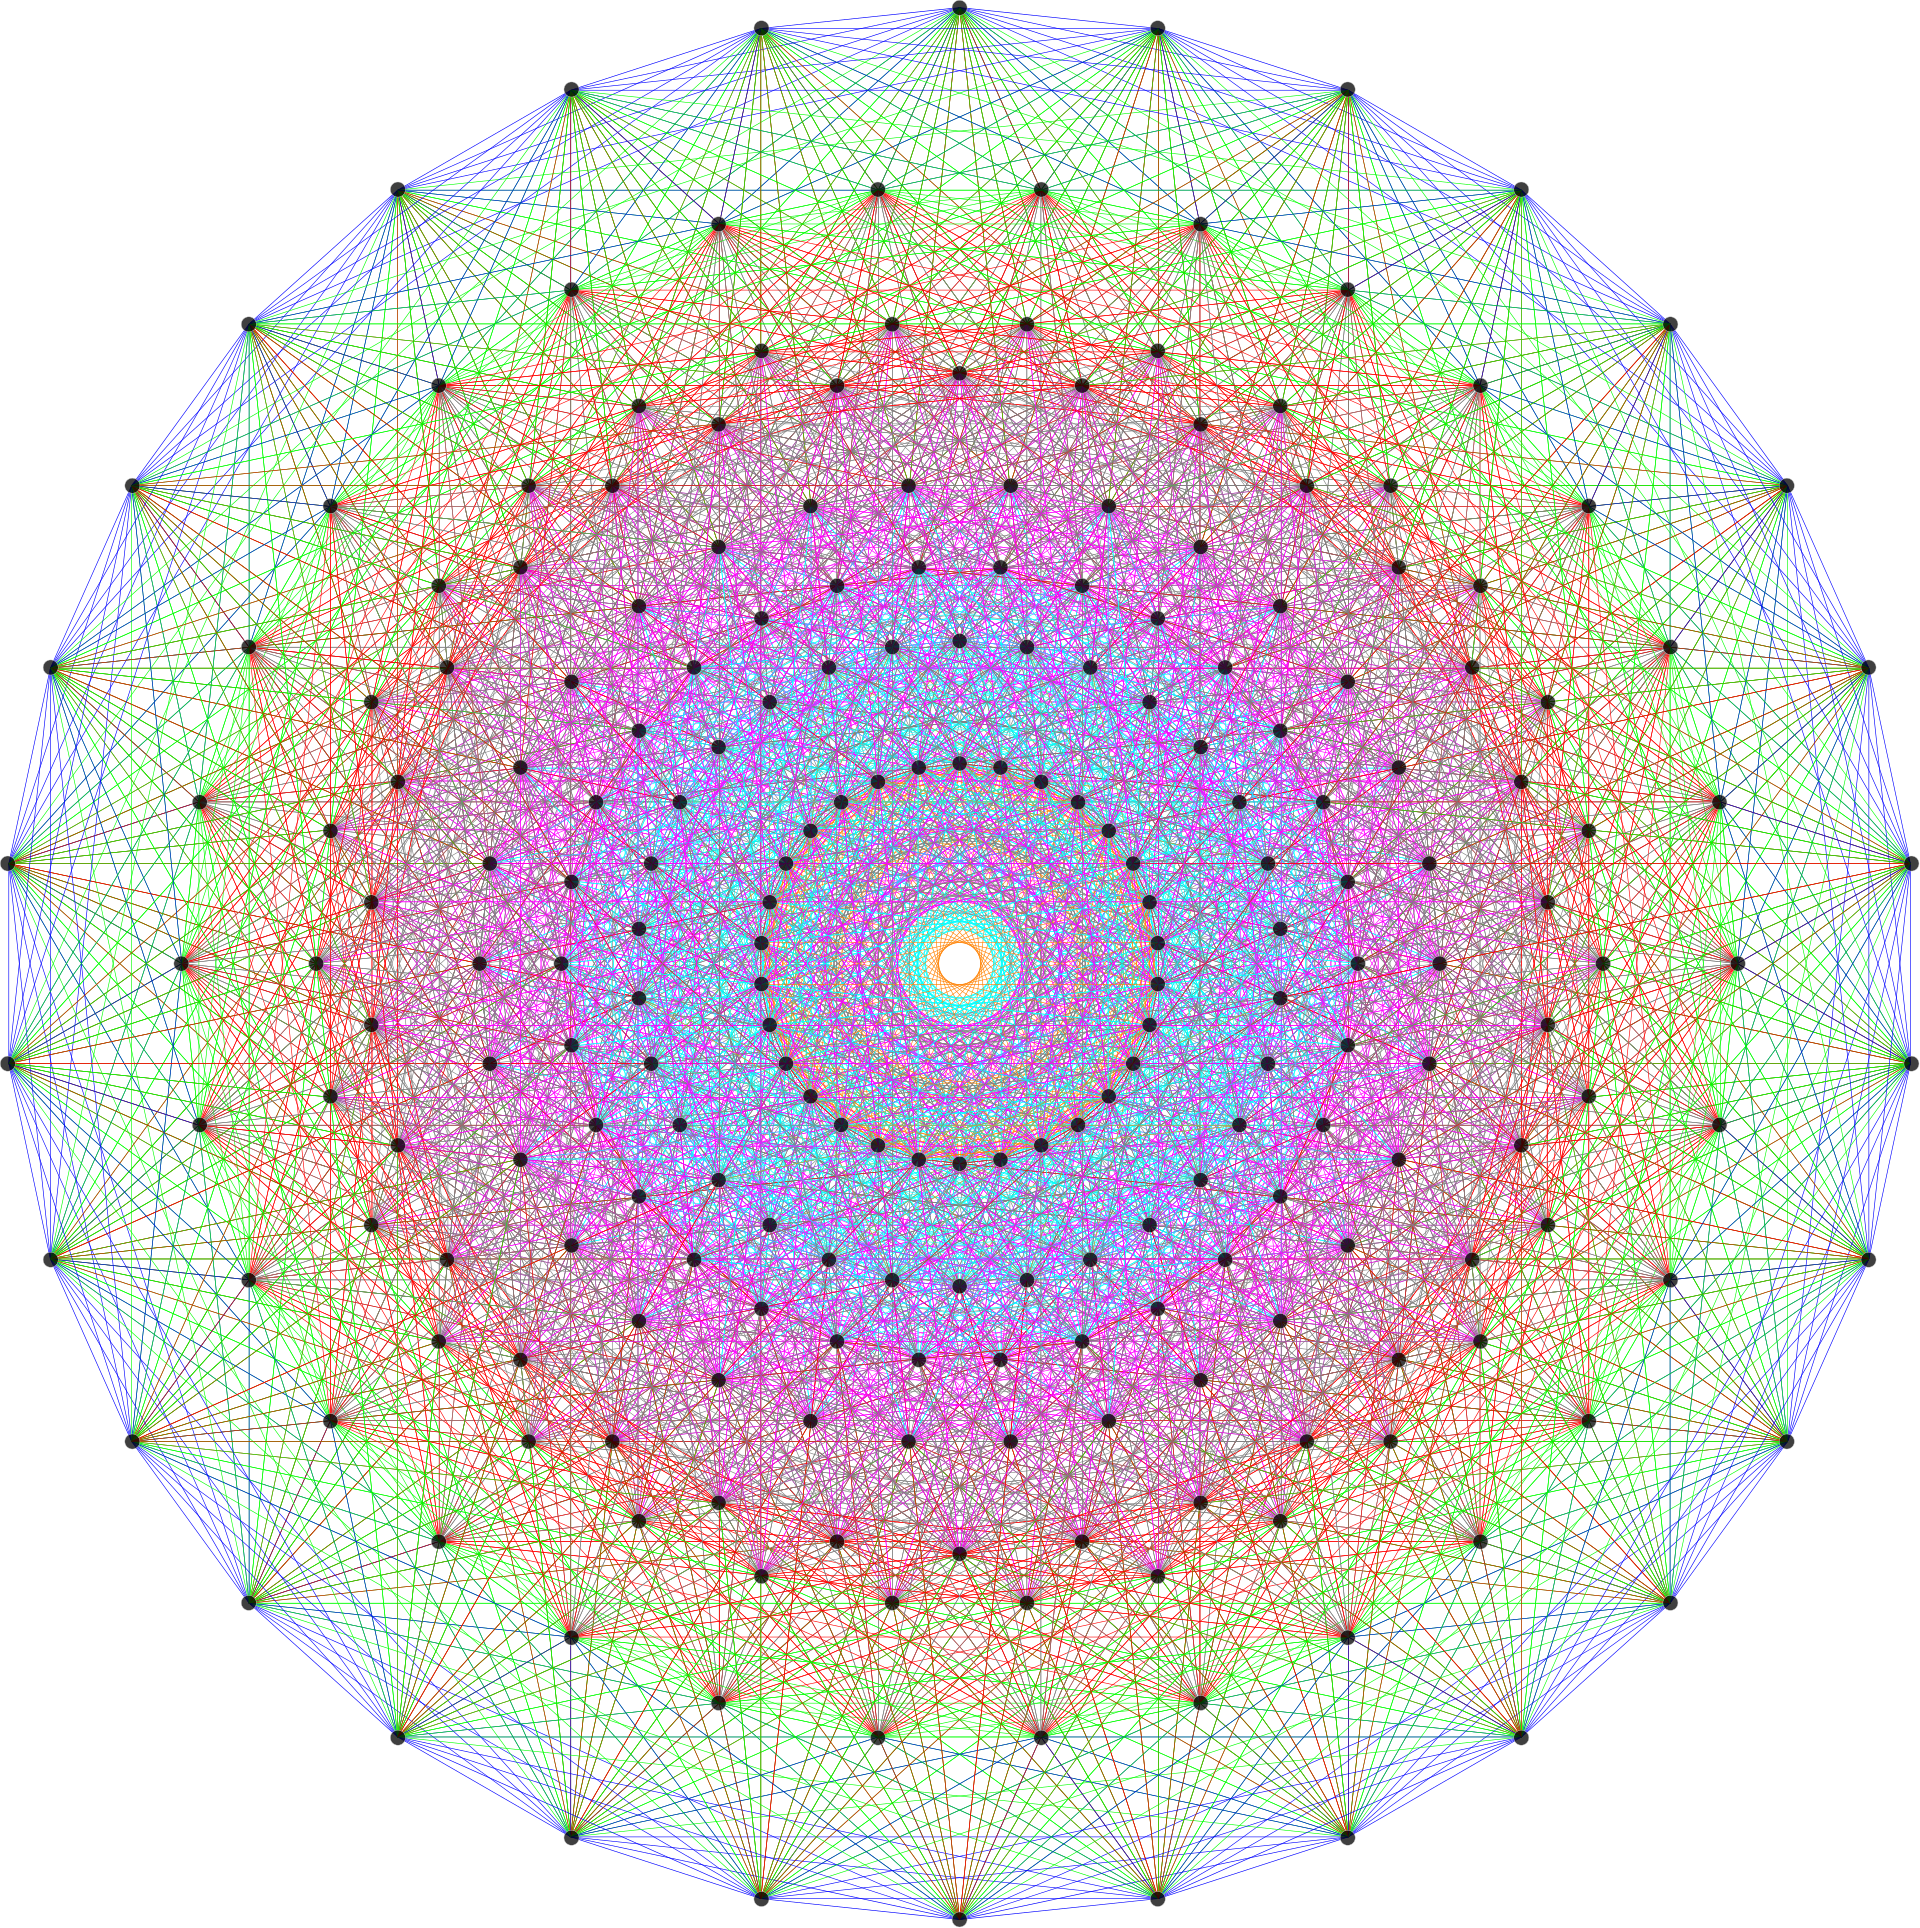
\includegraphics[scale=0.2]{cover}}
\date{}

\setlength{\abovedisplayskip}{10pt}
\setlength{\belowdisplayskip}{10pt}
\setlength{\abovedisplayshortskip}{5pt}
\setlength{\belowdisplayshortskip}{5pt}
\setlength\parindent{0pt}
\setlength{\jot}{5pt}

\maketitle
\tableofcontents

\part{Basic Mathematics}

\chapter{Axiomatic Set Theory}
\input{chapters/1.axiomatic_set_theory}

\chapter{Algebraic Structures}
\section{Algebraic Structures}

\bd [Algebraic Structures]
A set $A$ (called the underlying set, carrier set or domain), together with a collection of maps (called operations) on $A$ of finite arity (typically binary operations), and a finite set of identities, known as axioms, that these operations must satisfy, is called an \textbf{algebraic structure}. Some algebraic structures also involve another set (called the scalar set).
\ed

Examples of algebraic structures with a single underlying set include groups,fields and rings. Examples of algebraic structures with two underlying sets include vector spaces, modules, and algebras. In this section we will review the most important algebraic structures for our purposes. \\

One has to be careful with the terminology since it changes depending on the area of mathematics. For example, in the context of universal algebra, the set $A$ with this structure is called an algebra, while, in other contexts, it is (somewhat ambiguously) called an algebraic structure, the term algebra being reserved for specific algebraic structures that are vector spaces over a field or modules over a commutative ring. \\

The properties of specific algebraic structures are studied in abstract algebra. The general theory of algebraic structures has been formalized in universal algebra. The language of category theory is used to express and study relationships between different classes of algebraic and non-algebraic objects. This is because it is sometimes possible to find strong connections between some classes of objects, sometimes of different kinds. For example, Galois theory establishes a connection between certain fields and groups: two algebraic structures of different kinds.

\section{Groups}

\bd [Group]
A \textbf{group}\index{field (algebraic)} is a tuple $(G,\cdot)$, where $G$ is a set (called the underlying set of the group) and $\cdot$ is a map (called operation) $G\times G \to G$ satisfying the following four group axioms:
\begin{itemize}
\item Closure: $\forall \, a,b \in G : a \cdot b \in G$;
\item Associativity: $\forall \, a,b,c \in G : (a \cdot b) \cdot c=a \cdot (b \cdot c)$;
\item Neutral Element: $\exists \, e \in G : \forall \, a \in G : a \cdot e = e \cdot a=a$;
\item Inverse Element: $\forall \, a \in G : \exists \, a^{-1} \in G : a \cdot a^{-1} =a^{-1}  \cdot a = e$;
\end{itemize}
\ed

The identity element $e$ of a group $G$ is often written as $1$ a notation inherited from the multiplicative identity. If a group is abelian, then one may choose to denote the group operation by $+$ and the identity element by $0$.\\

The result of the group operation may depend on the order of the operands. In other words, the result of combining element $a$ with element $b$ need not yield the same result as combining element $b$ with element $a$, so the equation $a \cdot b = b \cdot a$ may not be true for every two elements $a$ and $b$.

\bd [Abelian Group]
A group $G$ is called \textbf{Abelian} if on top of the four group axioms it also satisfies the axiom of commutativity:
\begin{itemize}
\item Commutativity: $\forall \, a,b \in G : a \cdot b = b \cdot a$;
\end{itemize}
\ed

Commutativity always holds in the group of integers under addition, because $a + b = b + a$ for any two integers (commutativity of addition). The symmetry group is an example of a group that is not abelian.

\section{Fields}

\bd [Field]
An \textbf{(algebraic) field}\index{field (algebraic)} is a triple $(K,+,\cdot)$, where $K$ is a set and $+,\cdot$ are maps $K\times K \to K$ satisfying the following axioms:
\begin{itemize}
\item $(K,+)$ is an abelian group, i.e.
\ben
\item[i)] Closure: $\forall \, a,b \in K : a + b \in K$;
\item[ii)] Associativity: $\forall \, a,b,c \in K : (a+b)+c=a+(b+c)$;
\item[iii)] Neutral Element: $\exists \, 0 \in K : \forall \, a \in K : a+0=0+a=a$;
\item[iv)] Inverse Element: $\forall \, a \in K : \exists \, {-a} \in K : a+(-a)=(-a)+a=0$;
\item[v)] Commutativity: $\forall \, a,b \in K : a+b=b+a$;
\een
\item $(K^*,\cdot)$, where $K^*:=K\sm\{0\}$, is an abelian group, i.e.
\ben
\item[vi)] Closure: $\forall \, a,b \in K^* : a \cdot b \in K^*$;
\item[vii)] Associativity: $\forall \, a,b,c \in K^* : (a\cdot b)\cdot c=a\cdot (b\cdot c)$;
\item[viii)] Neutral Element: $\exists \, 1 \in K^* : \forall \, a \in K^* : a\cdot 1=1\cdot a=a$;
\item[ix)] Inverse Element: $\forall \, a \in K^* : \exists \, a^{-1} \in K^* : a\cdot a^{-1}=a^{-1} \cdot a=1$;
\item[x)] Commutativity: $\forall \, a,b \in K^* : a\cdot b=b\cdot a$;
\een
\item the maps $+$ and $\cdot$ satisfy the distributive property:
\ben
\item[xi)] $\forall \, a,b,c \in K : (a+ b)\cdot c=a\cdot c + b\cdot c$;
\een
\end{itemize}
\ed

\br
In the above definition, we included axiom v for the sake of clarity, but in fact it can be proven starting from the other axioms.
\er

\section{Vector Spaces}

\bd [K-Vector Space]
Let $(K,+,\cdot)$ be a field. A $K$\textbf{-vector space}\index{vector space}, or \textbf{vector space over $K$} or \textbf{linear space over $K$} is a triple $(V,\oplus,\odot)$, where $V$ is a set and 
\bi{rl}
\oplus &\cl V\times V \to V\\
\odot  &\cl K\times V \to V
\ei
are maps satisfying the following axioms:
\begin{itemize}
\item $(V,\oplus)$ is an abelian group i.e.
\ben
\item[i)] Closure: $\forall \, v,w \in V : v \oplus w \in K$;
\item[ii)] Associativity: $\forall \, v,w,z \in V : (v \oplus w) \oplus z = v \oplus (w \oplus z)$;
\item[iii)] Neutral Element: $\exists \, 0 \in V : \forall \, v \in V : v \oplus 0 = 0 \oplus v = v$;
\item[iv)] Inverse Element: $\forall \, v \in V : \exists \, -v \in V : v \oplus (-v) = (-v) \oplus v = 0$;
\item[v)] Commutativity: $\forall \, v,w \in V : v \oplus w = w \oplus v$;
\een
\item the map $\odot$ is an \emph{action} of $K$ on $(V,\oplus)$:
\ben
\item[vi)] Distributivity Of Scalar Multiplication - Vector Addition: $\forall \, \lambda \in K : \forall \, v,w \in V : \lambda\odot(v\oplus w)=(\lambda\odot v)\oplus (\lambda\odot w)$;
\item[vii)] Distributivity Of Scalar Multiplication - Field Addition: $\forall \, \lambda,\mu \in K : \forall \, v \in V : (\lambda+\mu)\odot v= (\lambda \odot v) \oplus (\mu \odot v)$;
\item[viii)] Compatibility Of Scalar Multiplication - Field Multiplication $\forall \, \lambda,\mu \in K : \forall \, v \in V : (\lambda\cdot\mu)\odot v= \lambda \odot (\mu \odot v)$;
\item[ix)] Neutral Element Of Scalar Multiplication $\forall \, v \in V : 1\odot v = v$.
\een
\end{itemize}
\ed

The elements of a vector space are called \emph{vectors}, while the elements of $K$ are often called \emph{scalars}, and the map $\odot$ is called \emph{scalar multiplication}.

\subsection{Linear Maps}

As usual by now, we will look at the structure-preserving maps between vector spaces.

\bd [Linear Maps]
Let $(V,\oplus,\odot)$, $(W,\boxplus,\boxdot)$ be vector spaces over the same field $K$ and let $f\cl V\to W$ be a map. We say that $f$ is a \textbf{linear map}\index{linear map}\index{map!linear}, and we denote it as $f\cl V\xrightarrow{\sim}W$, if for all $v_1,v_2\in V$ and all $\lambda \in K$
\bse
f((\lambda\odot v_1)\oplus v_2) = (\lambda\boxdot f( v_1))\boxplus f(v_2).
\ese
\ed

From now on, we will drop the special notation for the vector space operations and suppress the dot for scalar multiplication. For instance, we will write the equation above as $f(\lambda v_1+v_2)=\lambda f(v_1)+f(v_2)$, hoping that this will not cause any confusion.

\bd [$\mathrm{Hom}(V,W)$]
Let $V$ and $W$ be vector spaces over the same field $K$. We define the set $\mathrm{Hom}(V,W)$ as the set of all linear maps between $V$ and $W$:
\bse
\mathrm{Hom}(V,W) := \{f \mid f\cl V\xrightarrow{\sim}W \}
\ese
\ed
$\mathrm{Hom}(V,W)$ can itself be made into a vector space over $K$ by defining:
\bi{rrCl}
\diamondplus \cl &\mathrm{Hom}(V,W) \times \mathrm{Hom}(V,W) &\to &\mathrm{Hom}(V,W)\\
& (f,g) & \mapsto & f \diamondplus g
\ei
where
\bi{rcCl}
f \diamondplus g \cl &V  &\xrightarrow{\sim} &W\\
& v & \mapsto & (f \diamondplus g)(v) := f(v)+g(v),
\ei 
and
\bi{rrCl}
\diamonddot \cl &K \times \mathrm{Hom}(V,W) &\to &\mathrm{Hom}(V,W)\\
& (\lambda,f) & \mapsto & \lambda \diamonddot f
\ei
where
\bi{rcCl}
\lambda \diamonddot f \cl &V  &\xrightarrow{\sim} &W\\
& v & \mapsto & (\lambda \diamonddot f)(v) := \lambda f(v).
\ei 
It is easy to check that both $f \diamondplus g$ and $\lambda \diamonddot f$ are indeed linear maps from $V$ to $W$. For instance, we have:
\bi{rCl"s}
(\lambda \diamonddot f)(\mu v_1+v_2) & = &  \lambda f(\mu v_1+v_2) & (by definition)\\
& = &  \lambda (\mu f( v_1)+f(v_2)) & (since $f$ is linear)\\
& = &  \lambda \mu f( v_1)+\lambda f(v_2) & (by axioms i and iii)\\
& = & \mu \lambda f( v_1)+\lambda f(v_2) & (since $K$ is a field)\\
& = & \mu (\lambda \diamonddot f)( v_1)+(\lambda \diamonddot f)(v_2) & 
\ei
so that $\lambda \diamonddot f\in \mathrm{Hom}(V,W)$. One should also check that $\diamondplus$ and $\diamonddot$ satisfy the vector space axioms.

\bd [Endomorphisms]
Let $V$ be a vector space. An \textbf{endomorphism}\index{endomorphism} of $V$ is a linear map $V\to V$. 
\ed

\bd [$\mathrm{End}(V)$]
Let $V$ be a vector space. We define the set $\mathrm{End}(V)$ as the set of all endomorphisms of $V$:  
\bse
\mathrm{End}(V):=\mathrm{Hom}(V,V)
\ese
\ed

\vspace{5pt}

It is easy to show that $\mathrm{End}(V)$ can again itself be made into a vector space over $K$.

\bd [Linear Isomorphism]
A bijective linear map is called a \textbf{linear isomorphism}\index{isomorphism!of vector spaces} of vector spaces.
\ed

\bd [Isomorphic Vector Spaces]
Two vector spaces are said to be \textbf{isomorphic} if there exists a linear isomorphism between them. We write $V\cong_\mathrm{vec}W$.
\ed

\bd [Automorphism]
Let $V$ be a vector space. An \textbf{automorphism}\index{automorphism} of $V$ is a linear isomorphism $V\to V$.
\ed

\bd [$\mathrm{Aut}(V)$]
Let $V$ be a vector space. We define the set $\mathrm{Aut}(V)$ as the set of all automorphisms of $V$:
\bse
\mathrm{Aut}(V):=\{f \in \mathrm{End}(V) \mid f \text{ is an isomorphism}\}
\ese
\ed

\br
Note that $\mathrm{Aut}(V)$ \textbf{cannot} be made into a vector space . It is however a group under the operation of composition of linear maps.
\er

\bd [Dual Vector Space]
Let $V$ be a vector space over $K$. The \textbf{dual}\index{vector space!dual}\index{dual space} vector space to $V$ is
\bse
V^*:=\Hom(V,K),
\ese
where $K$ is considered as a vector space over itself.
\ed

The dual vector space to $V$ is the vector space of linear maps from $V$ to the underlying field $K$, which are variously called \emph{linear functionals}, \emph{covectors}\index{covector}, or \emph{one-forms} on $V$. The dual plays a very important role, in that from a vector space and its dual, we will construct the tensor products.

\subsection{Basis Of Vector Spaces}

Given a vector space without any additional structure, the only notion of basis that we can define is a so-called Hamel basis.

\bd [Hamel Basis]
Let $(V,+,\cdot)$ be a vector space over $K$. A subset $\mathcal{B}\se V$ is called a \textbf{Hamel basis}\index{Hamel basis}\index{vector space!basis} for $V$ if 
\begin{itemize}
\item every finite subset $\{b_1,\ldots,b_N\}$ of $\mathcal{B}$ is linearly independent, i.e.\
\bse
\sum_{i=1}^N \lambda^ib_i = 0 \ \imp \ \lambda^1 = \cdots = \lambda^N = 0;
\ese
\item $\mathcal{B}$ is a \emph{generating} or \emph{spanning set} of $V$, i.e.\
\bse
\forall \, v \in V : \exists \, v^1,\ldots,v^M\in K : \exists \, b_1,\ldots,b_M \in \mathcal{B}:v=\ds \sum_{i=1}^Mv^ib_i.
\ese
\end{itemize}
\ed
\br
We can write the second condition more succinctly by defining
\bse
\lspan_K(\mathcal{B}) := \bigg\{\sum_{i=1}^n\lambda^ib_i \ \Big| \ \lambda^i\in K \land b_i\in \mathcal{B} \land n\geq 1\bigg\}
\ese
and thus writing $V = \lspan_K(\mathcal{B})$.
\er
\br
Note that we have been using superscripts for the elements of $K$, and these should not be confused with exponents.
\er
The following characterisation of a Hamel basis is often useful.
\bp
Let $V$ be a vector space and $\mathcal{B}$ a Hamel basis of $V$. Then $\mathcal{B}$ is a minimal spanning and maximal independent subset of $V$, i.e., if $S\se V$, then
\begin{itemize}
\item $\lspan(S) = V\ \Rightarrow \ |S| \geq |\mathcal{B}|$;
\item $S$ is linearly independent $\ \Rightarrow\ |S| \leq |\mathcal{B}|$. 
\end{itemize}
\ep

\bd [Dimension Of Vector Space]
Let $V$ be a vector space. The \textbf{dimension}\index{dimension!vector space}\index{vector space!dimension} of $V$ is $\dim V := |\mathcal{B}|$, where $\mathcal{B}$ is a Hamel basis for $V$.
\ed
Even though we will not prove it, it is the case that every Hamel basis for a given vector space has the same cardinality, and hence the notion of dimension is well-defined.

\bp
If $\dim V < \infty$ and $S\se V$, then we have the following:
\begin{itemize}
\item if $\lspan_K(S) = V$ and $|S| = \dim V$, then $S$ is a Hamel basis of $V$;
\item if $S$ is linearly independent and $|S| = \dim V$, then $S$ is a Hamel basis of $V$. 
\end{itemize}
\ep

\begin{theorem}
If $\dim V < \infty$, then $(V^*)^*\cong_\mathrm{vec}V$.
\end{theorem}

\br
Note that while we need the concept of basis to state this result (since we require $\dim V < \infty$), the isomorphism that we have constructed is independent of any choice of basis.
\er

\br
While a choice of basis often simplifies things, when defining new objects it is important to do so without making reference to a basis. If we do define something in terms of a basis (e.g.\ the dimension of a vector space), then we have to check that the thing is well-defined, i.e.\ it does not depend on which basis we choose.
\er

If $V$ is finite-dimensional, then $V^*$ is also finite-dimensional and $V\cong_\mathrm{vec}V^*$. Moreover, given a basis $\mathcal{B}$ of $V$, there is a spacial basis of $V^*$ associated to $\mathcal{B}$.

\bd [Dual Basis]
Let $V$ be a finite-dimensional vector space with basis $\mathcal{B}=\{e_1,\ldots,e_{\dim V}\}$. The \textbf{dual basis} to $\mathcal{B}$ is the unique basis $\mathcal{B'}=\{\epsilon^1,\ldots,\epsilon^{\dim V}\}$ of $V^*$ such that
\bse
\forall \, 1\leq i,j \leq \dim V :\quad  \epsilon^i(e_j) = \delta^i_j := \begin{cases}1 \quad \text{if }i=j\\0 \quad \text{if }i\neq j\end{cases}
\ese
\ed

\br
If $V$ is finite-dimensional, then $V$ is isomorphic to both $V^*$ and $(V^*)^*$. In the case of $V^*$, an isomorphism is given by sending each element of a basis $\mathcal{B}$ of $V$ to a different element of the dual basis $\mathcal{B}'$, and then extending linearly to $V$. You will (and probably already have) read that a vector space is \emph{canonically} isomorphic to its double dual, but \emph{not} canonically isomorphic to its dual, because an arbitrary choice of basis on $V$ is necessary in order to provide an isomorphism. 
\er

\subsection{Change Of Basis}

Let $V$ be a vector space over $K$ with $d=\dim V < \infty$ and let $\{e_1,\ldots,e_d\}$ be a basis of $V$. Consider a new basis $\{\widetilde e_1,\ldots,\widetilde e_d\}$. Since the elements of the new basis are also elements of $V$, we can expand them in terms of the old basis. We have:
\bse
\widetilde e_i = \sum_{j=1}^d A^j_{\phantom{j} i}\, e_j \qquad \text{for }1\leq i \leq d.
\ese
for some $A^j_{\phantom{j}i}\in K$. Similarly, we have
\bse
e_i = \sum_{j=1}^d B^j_{\phantom{j} i}\, \widetilde e_j \qquad \text{for }1\leq i \leq d.
\ese
for some $B^j_{\phantom{j}i}\in K$. It is a standard linear algebra result that the matrices $A$ and $B$, with entries $A^j_{\phantom{j}i}$ and $B^j_{\phantom{j}i}$ respectively, are invertible and, in fact, $A^{-1}=B$. \\

Once we have a basis $\mathcal{B}$, the expansion of $v\in V$ in terms of elements of $\mathcal{B}$ is, in fact, unique. Hence we can meaningfully speak of the \emph{components}\index{components} of $v$ in the basis $\mathcal{B}$. The notion of coordinates can also be generalised to the case of tensors that we will define next.

\subsection{Tensors}

\bd [Bilinear Maps]
Let $V$, $W$, $Z$ be vector spaces over $K$. A map $f\cl V\times W \to Z$ is said to be \textbf{bilinear}\index{bilinear map}\index{map!bilinear} if
\begin{itemize}
\item $\forall \, w\in W:\forall \, v_1,v_2\in V: \forall \,\lambda \in K : f(\lambda v_1+v_2,w)=\lambda f(v_1,w)+f(v_2,w)$;
\item $\forall \, v\in V:\forall \, w_1,w_2\in W: \forall \,\lambda \in K : f(v,\lambda w_1+w_2)=\lambda f(v,w_1)+f(v,w_2)$;
\end{itemize}
i.e.\ if the maps $v\mapsto f(v,w)$, for any fixed $w$, and $w\mapsto f(v,w)$, for any fixed $v$, are both linear as maps $V\to Z$ and $W\to Z$, respectively.
\ed

\br
Compare this with the definition of a linear map $f\cl V\times W \xrightarrow{\sim} Z$:
\bse
\forall \, x,y\in V \times W : \forall \, \lambda \in K : f(\lambda x+y)=\lambda f(x)+f(y).
\ese
More explicitly, if $x=(v_1,w_1)$ and $y = (v_2,w_2)$, then:
\bse
f(\lambda (v_1,w_1)+(v_2,w_2))=\lambda f((v_1,w_1))+f((v_2,w_2)).
\ese
A bilinear map out of $V\times W$ is \emph{not} the same as a linear map out of $V\times W$. In fact, bilinearity is just a special kind of non-linearity.
\er

\be
The map $f\cl \R^2\to \R$ given by $(x,y)\mapsto x+y$ is linear but not bilinear, while the map $(x,y)\mapsto xy$ is bilinear but not linear.
\ee

We can immediately generalise the above to define \emph{multilinear} maps out of a Cartesian product of vector spaces.

\bd [Tensors]
Let $V$ be a vector space over $K$. A \textbf{$(p,q)$-tensor}\index{tensor} $T$ on $V$ is a multilinear map
\bse
T\cl \underbrace{V^*\times\cdots \times V^*}_{p \text{ copies}} \times \underbrace{V \times \cdots \times V}_{q \text{ copies}} \to K.
\ese
\ed

\br
By convention, a $(0,0)$ on $V$ is just an element of $K$, and hence $T^0_0V=K$.
\er

\bd [Covariant / Contravariant Tensor]
A type $(p,0)$ tensor is called a \textbf{covariant $p$-tensor}, while a tensor of type $(0,q)$ is called a \textbf{contravariant $q$-tensor}.
\ed

\bd [$T^p_q V$]
We define the set of all $(p,q)$-tensors $T$ as:
\bse
T^p_q V\index{$T^p_qV$} := \underbrace{V\otimes\cdots \otimes V}_{p \text{ copies}} \otimes \underbrace{V^* \otimes \cdots \otimes V^*}_{q \text{ copies}} := \{T\mid T \text{ is a $(p,q)$-tensor on }V\}. 
\ese
\ed

\br
Note that to define $T^p_q V$ as a set, we should be careful and invoke the principle of restricted comprehension, i.e.\ we should say where the $T$s are coming from. In general, say we want to build a set of maps $f\cl A\to B$ satisfying some property $p$. Recall that the notation $f\cl A \to B$ is hiding the fact that is a relation (indeed, a functional relation), and a relation between $A$ and $B$ is a subset of $A\times B$. Therefore, we ought to write:
\bse
\{f\in \cP(A\times B)\mid f\cl A\to B \text{ and } p(f)\}.
\ese
In the case of $T^p_q V$ we have:
\bse
T^p_q V := \big\{T \in \cP\bigl(\underbrace{V^*\times\cdots \times V^*}_{p \text{ copies}} \times \underbrace{V \times \cdots \times V}_{q \text{ copies}} \times K\bigr) \mid  T \text{ is a $(p,q)$-tensor on }V\big\},
\ese
although we will not write this down every time.
\er

The set $T^p_q V$ can be equipped with a $K$-vector space structure by defining
\bi{rrCl}
\oplus\cl &T^p_q V \times T^p_q V &\to &T^p_q V\\
& (T,S) & \mapsto & T \oplus S
\ei
and
\bi{rrCl}
\odot \cl &K \times T^p_q V &\to &T^p_q V\\
& (\lambda,T) & \mapsto & \lambda \odot T,
\ei
where $T \oplus S$ and $\lambda \odot T$ are defined pointwise, as we did with $\mathrm{Hom}(V,W)$. \\

We now define an important way of obtaining a new tensor from two given ones.

\bd [Tensor Product]
Let $T\in T^p_q V$ and $S\in T^r_s V$. The \textbf{tensor product}\index{tensor!product} of $T$ and $S$ is the tensor $T\otimes S\in T^{p+r}_{q+s}V$ defined by:
\bi{rl}
(T\otimes S)(\omega_1,\ldots,\omega_p,\omega_{p+1},\ldots,\omega_{p+r},v_1,&\ldots,v_q,v_{q+1},\ldots,v_{q+s})\\
:=T(\omega_1,\ldots,\omega_p,v_1,&\ldots,v_q)\,S(\omega_{p+1},\ldots,\omega_{p+r},v_{q+1},\ldots,v_{q+s}),
\ei
with $\omega_i\in V^*$ and $v_i\in V$.
\ed

Some examples are in order.

\be
\ben[label=\alph*)]
\item $T^0_1 V := \{T\mid T\cl V \xrightarrow{\sim} K\} = \mathrm{Hom}(V,K) =: V^*$. Note that here multilinear is the same as linear since the maps only have one argument.
\item $T^1_1V\equiv V\otimes V^*:=\{T\mid T\text{ is a bilinear map }V^*\times V \to K\}$. We claim that this is the same as $\mathrm{End}(V^*)$. Indeed, given $T\in  V\otimes V^*$, we can construct $\widehat T \in \mathrm{End}(V^*)$ as follows:
\bi{rrCl}
\widehat T \cl &V^* &\xrightarrow{\sim}& V^*\\
& \omega & \mapsto & T(-,\omega)
\ei
where, for any fixed $\omega$, we have
\bi{rrCl}
T (-,\omega) \cl &V &\xrightarrow{\sim}& K\\
& v & \mapsto & T(v,\omega).
\ei
The linearity of both $\widehat T$ and $T(-,\omega)$ follows immediately from the bilinearity of $T$. Hence $T(-,\omega)\in V^*$ for all $\omega$, and $\widehat T \in \mathrm{End}(V^*)$. This correspondence is invertible, since can reconstruct $T$ from $\widehat T$ by defining
\bi{rrCl}
T  \cl &V \times V^* &\to & K\\
& (v,\omega) & \mapsto & T(v,\omega):=(\widehat T(\omega))(v).
\ei
The correspondence is in fact linear, hence an isomorphism, and thus \bse
T^1_1V\cong_\mathrm{vec}\mathrm{End}(V^*).
\ese
\een

Other examples we would like to consider are
\ben[label=\alph*),start=3]
\item $T^0_1 V \stackrel{?}{\cong}_\mathrm{vec} V$: while you will find this stated as true in some physics textbooks, it is in fact \emph{not true} in general;
\item $T^1_1 V \stackrel{?}{\cong}_\mathrm{vec} \mathrm{End}(V)$: This is also not true in general;
\item $(V^*)^* \stackrel{?}{\cong}_\mathrm{vec} V$: This only holds if $V$ is finite-dimensional.
\een
\ee

\bd [Components Of A Tensor]
Let $V$ be a finite-dimensional vector space over $K$ with basis $\mathcal{B}=\{e_1,\ldots,e_{\dim V}\}$ and dual basis $\{\epsilon^1,\ldots,\epsilon^{\dim V}\}$ and let $T\in T^p_qV$. We define the \textbf{components}\index{tensor!components} of $T$ in the basis $\mathcal{B}$ to be the numbers
\bse
T^{a_1\ldots a_p}_{\phantom{a_1\ldots a_p}b_1\ldots b_q} := T(\epsilon^{a_1},\ldots,\epsilon^{a_p},e_{b_1},\ldots,e_{b_q})\in K,
\ese
where $1\leq a_i,b_j\leq \dim V$.
\ed

Just as with vectors, the components completely determine the tensor. Indeed, we can reconstruct the tensor from its components by using the basis:
\bse
T = \underbrace{\sum_{a_1=1}^{\dim V}\!\cdots\!\sum_{b_q=1}^{\dim V}}_{p+q \text{ sums}} T^{a_1\ldots a_p}_{\phantom{a_1\ldots a_p}b_1\ldots b_q} e_{a_1}\otimes\cdots\otimes e_{a_p} \otimes \epsilon^{b_1}\otimes \cdots\otimes \epsilon^{b_q},
\ese
where the $e_{a_i}$s are understood as elements of $T^1_0V\cong_\mathrm{vec}V$ and the $\epsilon^{b_i}s$ as elements of $T^0_1V\cong_\mathrm{vec}V^*$. Note that each summand is a $(p,q)$-tensor and the (implicit) multiplication between the components and the tensor product is the scalar multiplication in $T^p_q V$.

\subsection{Notational Conventions}
From now on, we will employ the Einstein's summation convention, which consists in suppressing the summation sign when the indices to be summed over each appear once as a subscript and once as a superscript in the same term. For example, we write
\bi{rcl}
v=v^ie_i \qquad &\text{and}& \qquad T=T^{ij}_{\phantom{ij}k}e_i\otimes e_j \otimes f^k
\ei
instead of
\bi{rcl}
v=\sum_{i=1}^dv^ie_i \qquad &\text{and}& \qquad T=\sum_{i=1}^d\sum_{j=1}^d\sum_{k=1}^d
T^{ij}_{\phantom{ij}k}e_i\otimes e_j \otimes f^k.
\ei

Indices that are summed over are called \emph{dummy indices}; they always appear in pairs and clearly it doesn't matter which particular letter we choose to denote them, provided it doesn't already appear in the expression. Indices that are not summed over are called \emph{free indices}; expressions containing free indices represent multiple expressions, one for each value of the free indices; free indices must match on both sides of an equation. The ranges over which the indices run are usually understood and not written out. \\

The convention on which indices go upstairs and which downstairs (which we have already been using) is that:
\begin{itemize}
\item the basis vectors of $V$ carry downstairs indices;
\item the basis vectors of $V^*$ carry upstairs indices;
\item all other placements are enforced by the Einstein's summation convention.
\end{itemize}
For example, since the components of a vector must multiply the basis vectors and be summed over, the Einstein's summation convention requires that they carry upstair indices.

\be
Using the summation convention, we have:
\ben[label=\alph*)]
\item $\epsilon^a(v) = \epsilon^a(v^be_b)=v^b\epsilon^a(e_b)=v^b\delta^a_b=v^a$;
\item $\omega(e_b)=(\omega_a\epsilon^a)(e_b)=\omega_a\epsilon^a(e_b)=\omega_b$;
\item $\omega(v)=\omega_a\epsilon^a(v^be_b)=\omega_av^a$;
\een
where $v\in V$, $\omega \in V^*$, $\{e_i\}$ is a basis of $V$ and $\{\epsilon^j\}$ is the dual basis to $\{e_i\}$.
\ee

\br
The Einstein's summation convention should only be used when dealing with linear spaces and multilinear maps. The reason for this is the following. Consider a map $\phi\cl V\times W \to Z$, and let $v=v^ie_i\in V$ and $w=w^i\widetilde e_i\in W$. Then we have:
\bse
\phi(v,w) = \phi\,\bigg({\color{lightgray}\sum_{i=1}^d}v^ie_i,{\color{lightgray}\sum_{j=1}^{\widetilde{d}}} w^j\widetilde e_j\bigg) = {\color{lightgray}\sum_{i=1}^d \sum_{j=1}^{\widetilde{d}}}\phi(v^ie_i,w^j\widetilde e_j)= {\color{lightgray}\sum_{i=1}^d \sum_{j=1}^{\widetilde{d}}}v^iw^j\phi(e_i,\widetilde e_j).
\ese
Note that by suppressing the greyed out summation signs, the second and third term above are indistinguishable. But this is only true if $\phi$ is bilinear! Hence the summation convention should not be used (at least, not without extra care) in other areas of mathematics.
\er

\br
Having chosen a basis for $V$ and the dual basis for $V^*$, it is very tempting to think of $v=v^ie_i\in V$ and $\omega=\omega_i\epsilon^i\in V^*$ as $d$-tuples of numbers. In order to distinguish them, one may choose to write vectors as \emph{columns} of numbers and covectors as \emph{rows} of numbers:
\bse
v =v^ie_i \quad \leftrightsquigarrow\quad v\ \hat{=} \left(
\ba{c}
v^1\\
\vdots\\
v^d
\ea
\right)
\ese
and
\bse
\omega =\omega_i\epsilon^i \quad \leftrightsquigarrow\quad \omega \ \hat{=} \ (\omega_1,\ldots,\omega_d).
\ese

\vspace{5pt}

Given $\phi\in\mathrm{End}(V)\cong_\mathrm{vec}T^1_1V$, recall that we can write $\phi = \phi^i_{\phantom{i}j}\, e_i\otimes \epsilon^j$, where $\phi^i_{\phantom{i}j}:=\phi(\epsilon^i,e_j)$ are the components of $\phi$ with respect to the chosen basis. It is then also very tempting to think of $\phi$ as a square array of numbers:
\bse
\phi = \phi^i_{\phantom{i}j}\, e_i\otimes \epsilon^j \quad \leftrightsquigarrow\quad \phi \ \hat{=} \left(
\ba{cccc}
\phi^1_{\phantom{1}1} & \phi^1_{\phantom{1}2} & \cdots & \phi^1_{\phantom{1}d}\\
\phi^2_{\phantom{2}1} & \phi^2_{\phantom{2}2} & \cdots & \phi^2_{\phantom{2}d}\\
\vdots & \vdots & \ddots & \vdots\\
\phi^d_{\phantom{d}1} & \phi^d_{\phantom{d}2} & \cdots & \phi^d_{\phantom{d}d} 
\ea
\right)
\ese

\vspace{5pt}

The convention here is to think of the $i$ index on $\phi^i_{\phantom{i}j}$ as a \emph{row index}, and of $j$ as a \emph{column index}.
\er

We cannot stress enough that this is pure convention. Its usefulness stems from the following example.

\be
If $\dim V<\infty$, then we have $\mathrm{End}(V)\cong_\mathrm{vec}T^1_1V$. Explicitly, if $\phi \in \mathrm{End}(V)$, we can think of $\phi \in T^1_1V$, using the same symbol, as
\bse
\phi(\omega,v):=\omega(\phi(v)).
\ese
Hence the components of $\phi\in\mathrm{End}(V)$ are $\phi^a_{\phantom{a}b}:=\epsilon^a(\phi(e_b))$. \\

Now consider $\phi,\psi\in\mathrm{End}(V)$. Let us determine the components of $\phi\circ \psi$. We have:
\bi{rCl}
(\phi\circ \psi)^a_{\phantom{a}b} &:=& (\phi\circ \psi)(\epsilon^a,e_b)\\
&:=&\epsilon^a( (\phi\circ \psi)(e_b))\\
&=& \epsilon^a( (\phi(\psi(e_b)))\\
&=& \epsilon^a(\phi(\psi^m_{\phantom{m}b}\,e_m))\\
&=& \psi^m_{\phantom{m}b} \epsilon^a( \phi(e_m))\\
&:=& \psi^m_{\phantom{m}b}\, \phi^a_{\phantom{a}m} .
\ei
The multiplication in the last line is the multiplication in the field $K$, and since that's commutative, we have $\psi^m_{\phantom{m}b}\, \phi^a_{\phantom{a}m}  = \phi^a_{\phantom{a}m} \, \psi^m_{\phantom{m}b}$. However, in light of the convention introduced in the previous remark, the latter is preferable. Indeed, if we think of the superscripts as row indices and of the subscripts as column indices, then $\phi^a_{\phantom{a}m} \, \psi^m_{\phantom{m}b}$ is the entry in row $a$, column $b$, of the matrix product $\phi\psi$. \\

Similarly, $\omega(v)=\omega_mv^m$ can be thought of as the \emph{dot product} $\omega \cdot v\equiv\omega^Tv$, and
\bse
\phi(v,w)=w_a\,\phi^a_{\phantom{a}b}\,v^b \quad   \leftrightsquigarrow\quad \omega^T\phi v.
\ese
The last expression is could mislead you into thinking that the transpose is a ``good'' notion, but in fact it is not. It is very bad notation. It almost pretends to be basis independent, but it is not at all. \\

The moral of the story is that you should try your best \emph{not} to think of vectors, covectors and tensors as arrays of numbers. Instead, always try to understand them from the abstract, intrinsic, component-free point of view.
\ee

As a final note in the notational conventions let's see the change of components under a change of basis using the new notation.\\

Recall that if $\{e_a\}$ and $\{\widetilde e_a\}$ are basis of $V$, we have
\bse
\widetilde e_a=A^b_{\phantom{b}a}e_b \qquad \text{and}  \qquad e_a=B^m_{\phantom{m}a}\widetilde e_m,
\ese
with $A^{-1}=B$. Note that in index notation, the equation $AB=I$ reads $A^a_{\phantom{a}m}B^m_{\phantom{m}b}=\delta^a_b$. \\

We now investigate how the components of vectors and covectors change under a change of basis. 
\ben[label=\alph*)]
\item Let $v=v^ae_a=\widetilde v^a\widetilde e_a\in V$. Then:
\bse
v^a = \epsilon^a(v) = \epsilon^a(\widetilde v^b\widetilde e_b) = \widetilde v^b
\epsilon^a(\widetilde e_b) = \widetilde v^b \epsilon^a(A^m_{\phantom{m}b}e_m) = A^m_{\phantom{m}b} \widetilde v^b\epsilon^a(e_m)=A^a_{\phantom{a}b} \widetilde v^b.
\ese
\item Let $\omega = \omega_a\epsilon^a = \widetilde \omega_a\widetilde \epsilon^a  \in V^*$. Then:
\bse
\omega_a := \omega(e_a) = \omega(B^m_{\phantom{m}a}\widetilde e_m) = B^m_{\phantom{m}a}\omega(\widetilde e_m) = B^m_{\phantom{m}a}\widetilde \omega_m .
\ese
\een
Summarising, for $v\in V$, $\omega \in V^*$ and $\widetilde e_a=A^b_{\phantom{b}a}e_b$, we have:
\bi{rClcrCl}
v^a & = & A^a_{\phantom{a}b} \widetilde v^b &\qquad & \omega_a &= & B^b_{\phantom{b}a}\widetilde \omega_b \\
\widetilde v^a & = & B^a_{\phantom{a}b}  v^b & & \widetilde \omega_a &= & A^b_{\phantom{b}a}\omega_b 
\ei
The result for tensors is a combination of the above, depending on the type of tensor.
\ben
\item[c)] Let $T\in T^p_qV$. Then:
\bse
T^{a_1\ldots a_p}_{\phantom{a_1\ldots a_p}b_1\ldots b_q} = A^{a_1}_{\phantom{a_1}m_1}\cdots A^{a_p}_{\phantom{a_p}m_p} B^{n_1}_{\phantom{n_1}b_1} \cdots B^{n_q}_{\phantom{n_q}b_q} \widetilde T^{m_1\ldots m_p}_{\phantom{m_1\ldots m_p}n_1\ldots n_q},
\ese
i.e.\ the upstair indices transform like vector indices, and the downstair indices transform like covector indices. 
\een

\section{Rings}

\bd [Ring]
A \textbf{ring}\index{ring} is a triple $(R,+,\cdot)$, where $R$ is a set and $+,\cdot\cl R\times R\to R$ are maps satisfying the following axioms
\begin{itemize}
\item $(R,+)$ is an abelian group:
\ben
\item[i)] Closure: $\forall \, a,b \in R : a + b \in R$;
\item[ii)] Associativity: $\forall \, a,b,c \in R : (a+b)+c=a+(b+c)$;
\item[iii)] Neutral Element: $\exists \, 0 \in R : \forall \, a \in R : a+0=0+a=a$;
\item[iv)] Inverse Element: $\forall \, a \in R : \exists \, {-a} \in R : a+(-a)=(-a)+a=0$;
\item[v)] Commutativity: $\forall \, a,b \in R : a+b=b+a$;
\een
\item the operation $\cdot$ is closed and associative in $R^*:=R\sm\{0\}$:
\ben
\item[vi)] Closure: $\forall \, a,b \in R^* : a \cdot b \in R^*$;
\item[vii)] Associativity: $\forall \, a,b,c \in R^* : (a\cdot b)\cdot c=a\cdot (b\cdot c)$;
\een
\item the maps $+$ and $\cdot$ satisfy the distributive properties:
\ben
\item[viii)] $\forall \, a,b,c \in R : (a+ b)\cdot c=a\cdot c + b\cdot c$;
\item[ix)] $\forall \, a,b,c \in R : a \cdot (b+c)=a\cdot b + a\cdot c$.
\een
\end{itemize}

Note that since $\cdot$ is not required to be commutative, axioms viii and ix are both necessary. In the case of fields where $\cdot$ was commutative, ix followed from viii and commutativity of $\cdot$.
\ed

\bd [Commutative / Unital / Division Rings]
A ring $(R,+,\cdot)$ is said to be
\begin{itemize}
\item \textbf{commutative} if $\ \forall \, a,b\in R : a\cdot b = b \cdot a$;
\item \textbf{unital} if $\ \exists\, 1\in R : \forall \, a\in R : 1\cdot a = a \cdot 1 = a$;
\item a \textbf{division} (or \textbf{skew}) \emph{ring} if it is unital and 
\bse
\forall\, a \in R\sm\{0\} : \exists \, a^{-1}\in R\sm\{0\}: \ a\cdot a^{-1}=a^{-1}\cdot a = 1.
\ese
\end{itemize}
\ed

In a unital ring, an element for which there exists a multiplicative inverse is said to be a \emph{unit}. The set of units of a ring $R$ is denoted by $R^*$ (not to be confused with the vector space dual) and forms a group under multiplication. Then, $R$ is a division ring iff $R^*=R\sm\{0\}$.

\be
The sets $\Z$, $\Q$, $\R$, and $\C$ are all rings under the usual operations. They are also all fields, except $\Z$.
\ee

In general, if $(A,+,\cdot,\bullet)$ is an algebra, then $(A,+,\bullet)$ is a ring.

\section{Modules}

\bd [$R$-Module]
Let $(R,+,\cdot)$ be a unital ring. An \textbf{$R$-module}\index{module} is a triple $(M,\oplus,\odot)$ where $M$ is a set and
\bi{rrCl}
\oplus \cl & M \times M & \to & M\\
\odot \cl & R \times M & \to & M
\ei
are maps satisfying the following axioms:
\begin{itemize}
\item $(M,\oplus)$ is an abelian group i.e
\ben
\item[i)] Closure: $\forall \, m,n \in M : m \oplus n \in M$;
\item[ii)] Associativity: $\forall \, m,n,s \in M : (m \oplus n) \oplus s = m \oplus (n \oplus s)$;
\item[iii)] Neutral Element: $\exists \, 0 \in M : \forall \, m \in M : m \oplus 0 = 0 \oplus m = m$;
\item[iv)] Inverse Element: $\forall \, m \in M : \exists \, -m \in M : m \oplus (-m) = (-m) \oplus m = 0$;
\item[v)] Commutativity: $\forall \, m,n \in M : m \oplus n = n \oplus m$;
\een
\item the map $\odot$ is an \emph{action} of $R$ on $(M,\oplus)$:
\ben
\item[vi)] Distributivity Of Scalar Multiplication - Vector Addition: $\forall \, r \in R : \forall \, m,n \in M : r \odot (m\oplus n) = (r \odot m) \oplus (r \odot n)$;
\item[vii)] Distributivity Of Scalar Multiplication - Field Addition: $\forall \, r,s \in K : \forall \, m \in V : (r+s)\odot m = (r\odot m)\oplus (s\odot m)$;
\item[viii)] Compatibility Of Scalar Multiplication - Field Multiplication $\forall \, r,s \in R : \forall \, m \in M : (r\cdot s)\odot m = r \odot (s\odot m)$;
\item[ix)] Neutral Element Of Scalar Multiplication $\forall \, m \in M : 1\odot m = m$.
\een
\end{itemize}
\ed

So, modules are simply vector spaces over rings instead of fields. For this reason, most definitions we had for vector spaces carry over unaltered to modules.

\be
Any ring $R$ is trivially a module over itself, in the sense that every field $K$ is a vector space over itself.
\ee

In the following, we will usually denote $\oplus$ by $+$ and suppress the $\odot$, as we did with vector spaces.\\

\bd [Direct Sum Of Modules]
The \textbf{direct sum} of two $R$-modules $M$ and $N$ is the $R$-module $M\oplus N$, which has $M\times N$ as its underlying set and operations (inherited from $M$ and $N$) defined component-wise. 
\ed

Note that while we have been using $\oplus$ to temporarily distinguish two ``plus-like'' operations in different spaces, the symbol $\oplus$ is the standard notation for the direct sum.

\bd [Finitely Generated / Free / Projective Modules]
An $R$-module $M$ is said to be
\begin{itemize}
\item \textbf{finitely generated} if it has a finite generating set;
\item \textbf{free} is it has a basis;
\item \textbf{projective} if it is a direct summand of a free $R$-module $F$, i.e.\
\bse
M \oplus Q = F
\ese
for some $R$-module $Q$.
\end{itemize}
\ed

\be
Clearly, every free module is also projective.
\ee

\bd [R-Linear Maps]
Let $M$ and $N$ be two $R$-modules. A map $f\cl M \to N$ is said to be an \textbf{$R$-linear map}, or an \textbf{$R$-module homomorphism}, if
\bse
\forall \, r\in R : \forall \, m_1,m_2\in M : \ f(rm_1 + m_2)=rf(m_1)+f(m_2),
\ese
where it should be clear which operations are in $M$ and which in $N$.
\ed

\bd [Module Isomorphisms]
A bijective module homomorphism is said to be a \textbf{module isomorphism}\index{isomorphism!of modules}.
\ed

\bd [Isomorphic Modules]
Two modulesare said to be \textbf{isomorphic} if there exists a module isomorphism between them. We write $M\cong_{\mathrm{mod}}N$.
\ed

\bp
If a finitely generated module $R$-module $F$ is free, and $d\in \N$ is the cardinality of a finite basis, then
\bse
F\cong_\mathrm{mod} = \underbrace{R\oplus\cdots\oplus R}_{d \text{ copies}} =: R^d.
\ese
\ep
One can show that if $R^d\cong_\mathrm{mod} R^{d'}$, then $d=d'$ and hence, the concept of dimension is well-defined for finitely generated, free modules.

\begin{theorem}
Let $P,Q$ be finitely generated (projective) modules over a commutative ring $R$. Then
\bse
\Hom_R(P,Q) := \{\phi\cl P \xrightarrow{\sim} Q \mid \phi \text{ \normalfont is $R$-linear}\}
\ese
is again a finitely generated (projective) $R$-module, with operations defined pointwise.
\end{theorem}

The proof is exactly the same as with vector spaces. As an example, we can use this to define the dual of a module.

\subsection{Basis Of Modules}

The key fact that sets modules apart from vector spaces is that, unlike a vector space, an $R$-module need not have a basis, unless $R$ is a division ring. This is actually a well-known theorem that we will state but not prove.

\begin{theorem}
\label{thm:everybasis}
If $D$ is a division ring, then any $D$-module $V$ admits a basis.
\end{theorem}

\bc
Every vector space has a basis, since any field is also a division ring.
\ec

\section{Algebras}

\bd [Algebra]
Let $K$ be a field, and let $A$ be a vector space over $K$ equipped with an additional bilinear map (called binary operation or product) $\bullet \cl A\times A \to A$. The quadruple $(A,+,\cdot,\bullet)$ is called an \textbf{algebra}\index{algebra} over a field $K$.
\ed

\bd [Associative / Unital / Commutative Algebra]
An algebra $(A,+,\cdot,\bullet)$ is said to be
\ben[label=\roman*)]
\item \textbf{Associative} if $\ \forall \, v,w,z\in A :  v\bullet (w\bullet z) = (v\bullet w)\bullet z$;
\item \textbf{Unital} if $\ \exists \, \mathbf{1} \in A : \forall \, v \in V : \mathbf{1}\bullet v = v \bullet \mathbf{1} = v$;
\item \textbf{Commutative} or \emph{abelian} if $\ \forall \, v,w\in A :  v\bullet w = w\bullet v$.
\een
\ed

\bd [Derivation]
Let $A$ and $B$ be algebras. A \textbf{derivation}\index{derivation} on $A$ is a linear map $D\cl A \xrightarrow{\sim}B$ satisfying the Leibniz rule
\bse
D(v\bullet_Aw)= D(v)\bullet_Bw +_B v \bullet_B D(w).
\ese
for all $v,w \in A$.
\ed

\section{Lie Algebras}

An important class of algebras, that we will also see later, are the so-called Lie algebras, in which the product $v\bullet w$ is denoted as $[v,w]$ called the ``commutator" or ``Lie bracket".  Let's first define it, and then use it to define the corresponding Lie algebra.

\bd [Lie Bracket]
Let $K$ be a field, $A$ be a vector space over $K$ and $v,w \in A$. The \textbf{Lie bracket}\index{Lie bracket} (or \textbf{commutator}) of $v$ and $w$ defined as
\bi{rrCl}
[v,w] \cl & A \times A & \to & A\\ 
& (v,w) & \mapsto & [v,w] :=v w  - w v
\ei
\ed

\bd [Lie Algebra]
A \textbf{Lie algebra}\index{Lie algebra} $A$ is an algebra whose product $[-,-]$, called \emph{Lie bracket}\index{Lie bracket}, satisfies
\ben[label=\roman*)]
\item bilinearity: $A \times A \to A$
\item antisymmetry: $\ \forall\, v\in A : [v,v]=0$;
\item the Jacobi identity\index{Jacobi identity}: $\ \forall\, v,w,z\in A : [v,[w,z]] + [w,[z,v]] + [z,[v,w]] = 0$.
\een
Note that the zeros above represent the additive identity element in $A$, not the zero scalar
\ed

The antisymmetry condition immediately implies $[v,w]=-[w,v]$ for all $v,w\in A$, hence a (non-trivial) Lie algebra cannot be unital.

\be
Let $V$ be a vector space over $K$. Then $(\End(V),+,\cdot,\circ)$ (where the product is simply the composition of endomorphisms) is an associative, unital, non-commutative algebra over $K$. Define:
\bi{rrCl}
[-,-] \cl &\End(V)\times \End(V) &\to& \End(V)\\
&(\phi,\psi) &\mapsto& [\phi,\psi] := \phi\circ\psi-\psi\circ\phi.
\ei
It is instructive to check that $(\End(V),+,\cdot,[-,-])$ is a Lie algebra over $K$. In this case, the Lie bracket is typically called the \emph{commutator}\index{commutator}.
\ee

In general, given an associative algebra $(A,+,\cdot,\bullet)$, if we define 
\bse
[v,w]:=v\bullet w-w\bullet v,
\ese
then $(A,+,\cdot,[-,-])$ is a Lie algebra.

\be
Consider again the Lie algebra $(\End(V),+,\cdot,[-,-])$ and fix $\xi \in \End(V)$. If we define
\bi{rrCl}
D_\xi := [\xi,-] \cl &\End(V) &\xrightarrow{\sim} &\End(V)\\
& \phi & \mapsto & [\xi,\phi],
\ei
then $D_\xi$ is a derivation on $(\End(V),+,\cdot,[-,-])$ since it is linear and
\bi{rCl"s}
D_\xi([\phi,\psi]) & := & [\xi,[\phi,\psi]]\\
& = & -[\psi,[\xi,\phi]] -[\phi,[\psi,\xi]]& (by the Jacobi identity)\\
& = & [[\xi,\phi],\psi]+[\phi,[\xi,\psi]] & (by antisymmetry)\\
& =: &  [D_\xi(\phi),\psi]+[\phi,D_\xi(\psi)].
\ei
This construction works in general Lie algebras as well.
\ee

Of course one can construct an algebra over a ring, by imposing all the axioms on a module instead of a vector space. Same definitions apply for an algebra over a ring with the appropriate changes when needed.

\subsection{Classification Of Lie Algebras}

One of the most important topics on Lie algebras is the classification of them. While it is possible to classify Lie algebras more generally, we will only consider the classification of finite-dimensional complex Lie algebras, i.e.\ Lie algebras $(L,[-,-])$ where $L$ is a finite-dimensional $\C$-vector space. 

If $A,B$ are Lie subalgebras of a Lie algebra $(L,[-,-])$ over $K$, then
\bse
[A,B] := \lspan_K\bigl(\{[x,y]\in L \mid x\in A \text{ and } y\in B\}\bigr)
\ese
is again a Lie subalgebra of $L$.

\bd
A Lie algebra $L$ is said to be \emph{abelian} if
\bse
\forall \, x,y \in L : \ [x,y] = 0.
\ese
Equivalently, $[L,L]=0$, where $0$ denotes the trivial Lie algebra $\{0\}$.
\ed
Abelian Lie algebras are highly non-interesting as Lie algebras: since the bracket is identically zero, it may as well not be there. Even from the classification point of view, the vanishing of the bracket implies that, given any two abelian Lie algebras, every linear isomorphism between their underlying vector spaces is automatically a Lie algebra isomorphism. Therefore, for each $n\in \N$, there is (up to isomorphism) only one abelian $n$-dimensional Lie algebra.
\bd
An \emph{ideal}\index{ideal} $I$ of a Lie algebra $L$ is a Lie subalgebra such that $[I,L]\se I$, i.e.\
\bse
\forall \, x\in I : \forall \, y\in L : \ [x,y]\in I.
\ese
The ideals $0$ and $L$ are called the \emph{trivial ideals} of $L$.
\ed

\bd
A Lie algebra $L$ is said to be 
\begin{itemize}
\item \emph{simple} if it is non-abelian and it contains no non-trivial ideals;
\item \emph{semi-simple} if it contains no non-trivial abelian ideals.
\end{itemize}
\ed

\br
Note that any simple Lie algebra is also semi-simple. The requirement that a simple Lie algebra be non-abelian is due to the $1$-dimensional abelian Lie algebra, which would otherwise be the only simple Lie algebra which is not semi-simple.
\er

\bd
Let $L$ be a Lie algebra. The Lie subalgebra
\bse
L':=[L,L]
\ese
is called the \emph{derived subalgebra}\index{derived subalgebra} of $L$.
\ed

We can form a sequence of Lie subalgebras
\bse
L \supseteq L' \supseteq L'' \supseteq \cdots \supseteq L^{(n)} \supseteq \cdots
\ese
called the \emph{derived series} of $L$.

\bd
A Lie algebra $L$ is \emph{solvable} if there exists $k\in \N$ such that $L^{(k)}=0$.
\ed

Recall that the direct sum of vector spaces $V\oplus W$ has $V\times W$ as its underlying set and operations defined componentwise.

\bd
Let $L_1$ and $L_2$ be Lie algebras. The \emph{direct sum} $L_1\oplus_\mathrm{Lie}L_2$ has $L_1\oplus L_2$ as its underlying vector space and Lie bracket defined as
\bse
[x_1+x_2,y_1+y_2]_{L_1\oplus_\mathrm{Lie}L_2} := [x_1,y_1]_{L_1} + [x_2,y_2]_{L_2}
\ese
for all $x_1,y_1\in L_1$ and $x_2,y_2\in L_2$. Alternatively, by identifying $L_1$ and $L_2$ with the subspaces $L_1\oplus 0$ and $0\oplus L_2$ of $L_1\oplus L_2$ respectively, we require
\bse
[L_1,L_2]_{L_1\oplus_\mathrm{Lie}L_2} = 0.
\ese
In the following, we will drop the ``Lie'' subscript and understand $\oplus$ to mean $\oplus_\mathrm{Lie}$ whenever the summands are Lie algebras.
\ed
There is a weaker notion than the direct sum, defined only for Lie algebras.
\bd
Let $R$ and $L$ be Lie algebras. The \emph{semi-direct sum} $R\oplus_s L$ has $R\oplus L$ as its underlying vector space and Lie bracket satisfying
\bse
[R,L]_{R \oplus_s L} \se R,
\ese
i.e.\ $R$ is an ideal of $R\oplus_s L$.
\ed

We are now ready to state Levi's decomposition theorem.

\begin{theorem}[Levi]
Any finite-dimensional complex Lie algebra $L$ can be decomposed as
\bse
L = R \oplus_s (L_1 \oplus\cdots  \oplus L_n)
\ese
where $R$ is a solvable Lie algebra and $L_1,\ldots,L_n$ are simple Lie algebras.
\end{theorem}

As of today, no general classification of solvable Lie algebras is known, except for some special cases (e.g. in low dimensions). In contrast, the finite dimensional, simple, complex Lie algebras have been classified completely. % From now on, we will assume our Lie algebras to be complex unless otherwise stated.

\bp
A Lie algebra is semi-simple if, and only if, it can be expressed as a direct sum of simple Lie algebras.
\ep

Hence, the simple Lie algebras are the basic building blocks from which one can build any semi-simple Lie algebra. Then, by Levi's theorem, the classification of simple Lie algebras easily extends to a classification of all semi-simple Lie algebras.

\subsection{The adjoint map and the Killing form}

\bd
Let $L$ be a Lie algebra over $k$ and let $x\in L$. The \emph{adjoint map}\index{adjoint map} with respect to $x$ is the $K$-linear map
\bi{rrCl}
\ad_x\cl & L & \xrightarrow{\sim} & L\\
& y & \mapsto & \ad_x(y):=[x,y].
\ei
\ed

The linearity of $\ad_x$ follows from the linearity of the bracket in the second argument, while the linearity in the first argument of the bracket implies that the map
\bi{rrCl}
\ad\cl & L & \xrightarrow{\sim} & \End(L)\\
& x & \mapsto & \ad(x):=\ad_x.
\ei
itself is also linear. In fact, more is true. Recall that $\End(L)$ is a Lie algebra with bracket
\bse
[\phi,\psi]:=\phi\circ\psi-\psi\circ\phi.
\ese
Then, we have the following.
\bp
The map $\ad\cl L \xrightarrow{\sim}  \End(L)$ is a Lie algebra homomorphism.
\ep
\bq
It remains to check that $\ad$ preserves the brackets. Let $x,y,z\in L$. Then
\bi{rCl"s}
\ad_{[x,y]}(z) & := & [[x,y],z] & (definition of $\ad$)\\
& = & -[[y,z],x]-[[z,x],y] & (Jacobi's identity)\\
& = & [x,[y,z]]-[y,[x,z]] & (anti-symmetry)\\
& = & \ad_x(\ad_y(z))-\ad_y(\ad_x(z)) \\
& = & (\ad_x\circ \ad_y-\ad_y\circ \ad_x)(z)\\
& = & [\ad_x, \ad_y](z).
\ei
Hence, we have $\ad([x,y])=[\ad(x),\ad(y)]$.
\eq

\bd
Let $L$ be a Lie algebra over $K$. The \emph{Killing form}\index{Killing form} on $L$ is the $K$-bilinear map
\bi{rrCl}
\kappa \cl & L\times L & \to & K \\
& (x,y) & \mapsto & \kappa(x,y):= \tr(\ad_x\circ\ad_y),
\ei
where $\tr$ is the usual trace on the vector space $\End(L)$.
\ed
Note that the Killing form is not a ``form'' in the sense that we defined previously. In fact, since $L$ is finite-dimensional, the trace is cyclic and thus $\kappa$ is symmetric, i.e.\
\bse
\forall \, x,y\in L : \ \kappa(x,y) = \kappa(y,x).
\ese
An important property of $\kappa$ is its associativity with respect to the bracket.
\bp
Let $L$ be a Lie algebra. For any $x,y,z\in L$, we have
\bse
\kappa([x,y],z)=\kappa(x,[y,z]).
\ese
\ep
\bq
This follows easily from the fact that $\ad$ is a homomorphism.
\bi{rCl}
\kappa([x,y],z) & := & \tr(\ad_{[x,y]}\circ\ad_z)\\
& = & \tr([\ad_x,\ad_y]\circ\ad_z)\\
& = & \tr((\ad_x \circ \ad_y-\ad_y\circ\ad_x)\circ\ad_z)\\
& = & \tr(\ad_x \circ \ad_y\circ\ad_z)-\tr(\ad_y\circ\ad_x\circ\ad_z)\\
& = & \tr(\ad_x \circ \ad_y\circ\ad_z)-\tr(\ad_x\circ\ad_z\circ\ad_y)\\
& = & \tr(\ad_x \circ\, (\ad_y\circ\ad_z-\ad_z\circ\ad_y))\\
& = & \tr(\ad_x \circ\, [\ad_y,\ad_z])\\
& = & \tr(\ad_x \circ \ad_{[y,z]})\\
& =: & \kappa(x,[y,z]),
\ei
where we used the cyclicity of the trace.
\eq

We can use $\kappa$ to give a further equivalent characterisation of semi-simplicity.

\bp[Cartan's criterion]\index{Cartan's criterion}
A Lie algebra $L$ is semi-simple if, and only if, the Killing form $\kappa$ is non-degenerate, i.e.\
\bse
(\forall \, y \in L : \kappa(x,y)=0) \Rightarrow x = 0.
\ese
\ep
Hence, if $L$ is semi-simple, then $\kappa$ is a pseudo inner product on $L$. Recall the following definition from linear algebra.

\bd
A linear map $\phi\cl V\xrightarrow{\sim}V$ is said to be \emph{symmetric} with respect to the pseudo inner product $B(-,-)$ on $V$ if
\bse
\forall \, v,w\in V : \ B(\phi(v),w)=B(v,\phi(w)).
\ese
If, instead, we have
\bse
\forall \, v,w\in V : \ B(\phi(v),w)=-B(v,\phi(w)),
\ese
then $\phi$ is said to be \emph{anti-symmetric} with respect to $B$.
\ed
The associativity property of $\kappa$ with respect to the bracket can be restated by saying that, for any $z\in L$, the linear map $\ad_z$ is anti-symmetric with respect to $\kappa$, i.e.\
\bse
\forall \, x,y\in L : \ \kappa(\ad_z(x),y) = - \kappa(x,\ad_z(y)). 
\ese

In order to do computations, it is useful to introduce a basis $\{E_i\}$ on $L$.
\bd
Let $L$ be a Lie algebra over $K$ and let $\{E_i\}$ be a basis. Then, we have
\bse
[E_i,E_j] = C^{k}_{\phantom{k}ij}E_k
\ese
for some $C^{k}_{\phantom{k}ij}\in K$. The numbers $C^{k}_{\phantom{k}ij}$ are called the \emph{structure constants}\index{structure constants} of $L$ with respect to the basis $\{E_i\}$.
\ed
In terms of the structure constants, the anti-symmetry of the Lie bracket reads
\bse
 C^{k}_{\phantom{k}ij} = - C^{k}_{\phantom{k}ji}
\ese
while the Jacobi identity becomes
\bse
C^{n}_{\phantom{n}im}C^{m}_{\phantom{m}jk} +  C^{n}_{\phantom{n}jm}C^{m}_{\phantom{m}ki} + C^{n}_{\phantom{n}km}C^{m}_{\phantom{m}ij} = 0.
\ese

We can now express both the adjoint maps and the Killing form in terms of components with respect to a basis.
\bp
Let $L$ be a Lie algebra and let $\{E_i\}$ be a basis. Then
\ben[label=\roman*)]
\item $(\ad_{E_i})^k_{\phantom{k}j} = C^{k}_{\phantom{k}ij}$
\item $\kappa_{ij}=C^m_{\phantom{m}ik}C^k_{\phantom{k}jm}$
\een
where $C^{k}_{\phantom{k}ij}$ are the structure constants of $L$ with respect to $\{E_i\}$.
\ep
\bq
\ben[label=\roman*)]
\item Denote by $\{\varepsilon^i\}$ the dual basis to $\{E_i\}$. Then, we have
\bi{rCl}
(\ad_{E_i})^k_{\phantom{k}j} &:=& \varepsilon^k(\ad_{E_i}(E_j)) \\
& = & \varepsilon^k ([E_i,E_j])\\
& = & \varepsilon^k (C^{m}_{\phantom{\,m}ij}E_m)\\
& = & C^{m}_{\phantom{m}ij}\varepsilon^k (E_m)\\
&=& C^{k}_{\phantom{k}ij},
\ei
since $\varepsilon^k(E_m)=\delta^k_m$.
\item Recall from linear algebra that if $V$ is finite-dimensional, for any $\phi\in\End(V)$ we have $\tr(\phi)=\Phi^k_{\phantom{k}k}$, where $\Phi$ is the matrix representing the linear map in any basis. Also, recall that the matrix representing $\phi\circ\psi$ is the product $\Phi\Psi$. Using these, we have
\bi{rCl}
\kappa_{ij} &:= & \kappa(E_i,E_j)\\
& = & \tr(\ad_{E_i}\circ\ad_{E_j})\\
& = & ( \ad_{E_i}\circ\ad_{E_j} )^k_{\phantom{k}k}\\
& = & ( \ad_{E_i})^m_{\phantom{m}k}(\ad_{E_j} )^k_{\phantom{k}m}\\
& = & C^m_{\phantom{m}ik}C^k_{\phantom{k}jm},
\ei 
where we used the same notation for the linear maps and their matrices.\qedhere
\een
\eq

\subsection{The fundamental roots and the Weyl group}

We will now focus on finite-dimensional semi-simple complex Lie algebras, whose classification hinges on the existence of a special type of subalgebra.

\bd
Let $L$ be a $d$-dimensional Lie algebra. A \emph{Cartan subalgebra}\index{Cartan subalgebra} $H$ of $L$ is a maximal Lie subalgebra of $L$ with the following property: there exists a basis $\{h_1,\ldots,h_r\}$ of $H$ which can be extended to a basis $\{h_1,\ldots,h_r,e_1,\ldots,e_{d-r}\}$ of $L$ such that $e_1,\ldots,e_{d-r}$ are eigenvectors of $\ad(h)$ for any $h\in H$, i.e.\
\bse
\forall \, h\in H : \exists \, \lambda_\alpha(h)\in \C : \ \ad(h)e_\alpha = \lambda_\alpha(h) e_\alpha,
\ese
for each $1\leq\alpha\leq d-r$.
\ed

The basis $\{h_1,\ldots,h_r,e_1,\ldots,e_{d-r}\}$ is known as a \emph{Cartan-Weyl basis}\index{Cartan-Weyl basis} of $L$.
%Of course, we would like to know when we can find such a subalgebra.

\begin{theorem}
Let $L$ be a finite-dimensional semi-simple complex Lie algebra. Then
\ben[label=\roman*)]
\item $L$ possesses a Cartan subalgebra;
\item all Cartan subalgebras of $L$ have the same dimension, called the \emph{rank} of $L$;
\item any of Cartan subalgebra of $L$ is abelian.
\een
\end{theorem}

Note that we can think of the $\lambda_\alpha$ appearing above as a map $\lambda_\alpha\cl H \to \C$. Moreover, for any $z\in \C$ and $h,h'\in H$, we have
\bi{rCl}
\lambda_\alpha(zh+h') e_\alpha  & = & \ad(zh+h') e_\alpha\\
& = & [zh+h',e_\alpha] \\
& = & z[h,e_\alpha] + [h',e_\alpha] \\
& = & z\lambda_\alpha(h)e_\alpha +\lambda_\alpha(h')e_\alpha\\
& = & (z\lambda_\alpha(h)+\lambda_\alpha(h')) e_\alpha,
\ei
Hence $\lambda_\alpha$ is a $\C$-linear map $\lambda_\alpha\cl H \xrightarrow{\sim}\C$, and thus $\lambda_\alpha\in H^*$.

\bd
The maps $\lambda_1,\ldots,\lambda_{d-r}\in H^*$ are called the \emph{roots}\index{root} of $L$. The collection
\bse
\Phi := \{\lambda_\alpha \mid 1\leq \alpha \leq d-r\} \se H^*
\ese
is called the \emph{root set} of $L$.
\ed

One can show that if $\lambda_\alpha$ were the zero map, then we would have $e_\alpha\in H$. Thus, we must have $0\notin \Phi$. Note that a consequence of the anti-symmetry of each $\ad(h)$ with respect to the Killing form $\kappa$ is that
\bse
\lambda \in \Phi\ \Rightarrow\ -\lambda\in \Phi.
\ese
Hence $\Phi$ is not a linearly independent subset of $H^*$.

\bd
A set of \emph{fundamental roots}\index{fundamental root} $\Pi:=\{\pi_1,\ldots,\pi_f\}$ is a subset $\Pi\se\Phi$ such that 
\ben[label=\alph*)]
\item $\Pi$ is a linearly independent subset of $H^*$;
\item for each $\lambda \in \Phi$, there exist $n_1,\ldots,n_f\in \N$ and $\varepsilon \in \{+1,-1\}$ such that
\bse
\lambda = \varepsilon \, \sum_{i=1}^f n_i \pi_i.
\ese
\een
\ed
We can write the last equation more concisely as $\lambda \in \lspan_{\varepsilon,\N}(\Pi)$. Observe that, for any $\lambda\in \Phi$, the coefficients of $\pi_1,\ldots,\pi_f$ in the expansion above always have the same sign. Indeed, we have $\lspan_{\varepsilon,\N}(\Pi)\neq \lspan_{\Z}(\Pi)$. 

\begin{theorem}
Let $L$ be a finite-dimensional semi-simple complex Lie algebra. Then
\ben[label=\roman*)]
\item a set $\Pi\se\Phi$ of fundamental roots always exists;
\item we have $\lspan_\C(\Pi) = H^*$, that is, $\Pi$ is a basis of $H^*$.
\een
\end{theorem}
\bc
We have $|\Pi| = r$, where $r$ is the rank of $L$.
\ec
\bq
Since $\Pi$ is a basis, $|\Pi| = \dim H^* = \dim H = r$.
\eq
We would now like to use $\kappa$ to define a pseudo inner product on $H^*$. We know from linear algebra that a pseudo inner product $B(-,-)$ on a finite-dimensional vector space $V$ over $K$ induces a linear isomorphism
\bi{rrCl}
i \cl & V & \xrightarrow{\sim} & V^*\\
& v & \mapsto & i(v) := B(v,-)
\ei
which can be used to define a pseudo inner product $B^*(-,-)$ on $V^*$ as
\bi{rrCl}
B^* \cl & V^*\times V^* & \to & K\\
& (\phi,\psi) & \mapsto & B^*(\phi,\psi) := B(i^{-1}(\phi),i^{-1}(\psi)).
\ei
We would like to apply this to the restriction of $\kappa$ to the Cartan subalgebra. However, a pseudo inner product on a vector space is not necessarily a pseudo inner product on a subspace, since the non-degeneracy condition may fail when considered on a subspace.
\bp
The restriction of $\kappa$ to $H$ is a pseudo inner product on $H$.
\ep
\bq
Bilinearity and symmetry are automatically satisfied. It remains to show that $\kappa$ is non-degenerate on $H$. 
\ben[label=\roman*)]
\item Let $\{h_1,\ldots,h_r,e_{r+1},\ldots,e_{d}\}$ be a Cartan-Weyl basis of $L$ and let $\lambda_\alpha\in \Phi$. Then
\bi{rCl}
\lambda_\alpha(h_j) \kappa(h_i,e_\alpha)& = & \kappa(h_i,\lambda_\alpha(h_j)e_\alpha)\\
& = & \kappa(h_i,[h_j,e_\alpha])\\
& = & \kappa([h_i,h_j],e_\alpha)\\
& = & \kappa(0,e_\alpha)\\
& = & 0.
\ei
Since $\lambda_\alpha \neq 0$, there is some $h_j$ such that $\lambda_\alpha(h_j)\neq 0$ and hence
\bse
\kappa(h_i,e_\alpha) = 0.
\ese
By linearity, we have $\kappa(h,e_\alpha)=0$ for any $h\in H$ and any $e_\alpha$.
\item Let $h\in H\se L$. Since $\kappa$ is non-degenerate on $L$, we have
\bse
\bigl(\forall \, x\in L : \kappa(h,x) = 0 \bigr) \Rightarrow h =0.
\ese
Expand $x\in L$ in the Cartan-Weyl basis as
\bse
x = h' + e  
\ese
where $h':=x^ih_i$ and $e:=x^\alpha e_\alpha$. Then, we have
\bse
\kappa(h,x) = \kappa(h,h') + x^\alpha\kappa(h,e_\alpha) = \kappa(h,h').
\ese
Thus, the non-degeneracy condition reads
\bse
\bigl(\forall \, h'\in H : \kappa(h,h') = 0 \bigr) \Rightarrow h =0,
\ese
which is what we wanted. \qedhere
\een
\eq

We can now define
\bi{rrCl}
\kappa^*\cl & H^* \times H^* & \to & \C\\
& (\mu,\nu)&\mapsto & \kappa^*(\mu,\nu):=\kappa(i^{-1}(\mu),i^{-1}(\nu)),
\ei
where $i\cl H \xrightarrow{\sim} H^*$ is the linear isomorphism induced by $\kappa$. 

\br
If $\{h_i\}$ is a basis of $H$, the components of $\kappa^*$ with respect to the dual basis satisfy 
\bse
(\kappa^*)^{ij}\kappa_{jk}=\delta^i_k.
\ese
Hence, we can write
\bse
\kappa^*(\mu,\nu)=(\kappa^*)^{ij}\mu_i\nu_j,
\ese
where $\mu_i:=\mu(h_i)$.
\er
We now turn our attention to the real subalgebra $H^*_\R:=\lspan_\R(\Pi)$. Note that  we have the following chain of inclusions
\bse
\Pi\se\Phi\se\lspan_{\varepsilon,\N}(\Pi) \se \underbrace{\lspan_\R(\Pi)}_{H_\R^*} \se \underbrace{\lspan_\C(\Pi)}_{H^*}.
\ese
The restriction of $\kappa^*$ to $H_\R^*$ leads to a surprising result.
\begin{theorem}
\ben[label=\roman*)]
\item For any $\alpha,\beta\in H_\R^*$, we have $\kappa^*(\alpha,\beta)\in \R$.
\item $\kappa^*\cl H_\R^*\times  H_\R^*\to \R$ is an inner product on $H_\R^*$.
\een
\end{theorem}
This is indeed a surprise! Upon restriction to $H_\R^*$, instead of being weakened, the non-degeneracy of $\kappa^*$ gets strengthened to positive definiteness. Now that we have a proper real inner product, we can define some familiar notions from basic linear algebra, such as lengths and angles.

\bd
Let $\alpha,\beta\in H_\R^*$. Then, we define
\ben[label=\roman*)]
\item the \emph{length} of $\alpha$ as $|\alpha|:=\sqrt{\kappa^*(\alpha,\alpha)}\,$;
\item the \emph{angle} between $\alpha$ and $\beta$ as $\ds \varphi := \cos^{-1}\biggl(\frac{\kappa^*(\alpha,\beta)}{|\alpha||\beta|}\biggr) $.
\een
\ed
We need one final ingredient for our classification result.
\bd
For any $\lambda\in \Phi\se H_\R^*$, define the linear map
\bi{rrCl}
s_\lambda \cl & H_\R^* & \xrightarrow{\sim} & H_\R^*\\
& \mu & \mapsto & s_\lambda(\mu),
\ei
where
\bse
s_\lambda(\mu):=\mu-2\frac{\kappa^*(\lambda,\mu)}{\kappa^*(\lambda,\lambda)}\,\lambda .
\ese
The map $s_\lambda$ is called a \emph{Weyl transformation} and the set
\bse
W:=\{s_\lambda \mid \lambda \in \Phi\}
\ese
is a group under composition of maps, called the \emph{Weyl group}\index{Weyl group}.
\ed

\begin{theorem}
\ben[label=\roman*)]
\item The Weyl group $W$ is generated by the fundamental roots in $\Pi$, in the sense that for some $1\leq n \leq r$, with $r=|\Pi|$,
\bse
\forall \, w \in W : \exists \, \pi_1,\ldots,\pi_n\in \Pi : \ w = s_{\pi_1} \circ s_{\pi_2} \circ\cdots  \circ s_{\pi_n} ;
\ese
\item Every root can be produced from a fundamental root by the action of $W$, i.e.\
\bse
\forall \, \lambda\in \Phi :\exists\, \pi\in \Pi :  \exists\, w\in W :\ \lambda = w(\pi);
\ese
\item The Weyl group permutes the roots, that is,
\bse
\forall \, \lambda \in \Phi : \forall \, w \in W : \ w(\lambda)\in \Phi.
\ese
\een
\end{theorem}

\subsection{Dynkin diagrams and the Cartan classification}

Consider, for any $\pi_i,\pi_j\in \Pi$, the action of the Weyl transformation
\bse
s_{\pi_i}(\pi_j) := \pi_j-2\frac{\kappa^*(\pi_i,\pi_j)}{\kappa^*(\pi_i,\pi_i)}\,\pi_i.
\ese
Since $s_{\pi_i}(\pi_j)\in\Phi$ and $\Phi\se\lspan_{\varepsilon,\N}(\Pi)$, for all $1\leq i\neq j\leq r$ we must have
\bse
-2\frac{\kappa^*(\pi_i,\pi_j)}{\kappa^*(\pi_i,\pi_i)}\in \N.
\ese
\bd
The \emph{Cartan matrix}\index{Cartan matrix} of a Lie algebra is the $r\times r$ matrix $C$ with entries
\bse
C_{ij} :=2\frac{\kappa^*(\pi_i,\pi_j)}{\kappa^*(\pi_i,\pi_i)},
\ese
where the $C_{ij}$ should not be confused with the structure constants $C^k_{\phantom{k}ij}$.
\ed
\begin{theorem}To every simple finite-dimensional complex Lie algebra there corresponds a unique Cartan matrix and vice versa (up to relabelling of the basis elements).
\end{theorem}
Of course, not every matrix can be a Cartan matrix. For instance, since $C_{ii}=2$ (no summation implied), the diagonal entries of $C$ are all equal to $2$, while the off-diagonal entries are either zero or negative. In general, $C_{ij} \neq C_{ji}$, so the Cartan matrix is not symmetric, but if $C_{ij}=0$, then necessarily $C_{ji}=0$.

We have thus reduced the problem of classifying the simple finite-dimensional complex Lie algebras to that of finding all the Cartan matrices. This can, in turn, be reduced to the problem of determining all the inequivalent Dynkin diagrams. 
\bd
Given a Cartan matrix $C$, the $ij$-th \emph{bond number} is
\bse
n_{ij}:= C_{ij} C_{ji} \qquad \text{(no summation implied)}.
\ese
\ed
Note that we have
\bi{rCl}
n_{ij} & = & 4\,\frac{\kappa^*(\pi_i,\pi_j)}{\kappa^*(\pi_i,\pi_i)}\,\frac{\kappa^*(\pi_j,\pi_i)}{\kappa^*(\pi_j,\pi_j)}\\
& = & 4\, \biggl(\frac{\kappa^*(\pi_i,\pi_j)}{|\pi_i||\pi_j|}\biggr)^2\\
& = & 4 \cos^2\varphi,
\ei
where $\varphi$ is the angle between $\pi_i$ and $\pi_j$. For $i\neq j$, the angle $\varphi$ is neither zero nor $180^\circ$, hence $0\leq \cos^2\varphi< 1$, and therefore
\bse
n_{ij}\in \{0,1,2,3\}.
\ese
Since $C_{ij}\leq 0$ for $i\neq j$, the only possibilities are
\begin{center}
%\def\arraystretch{1}
%\setlength\tabcolsep{10pt}
\begin{tabular}{ cc | c}
$C_{ij}$ & $C_{ji}$ & $n_{ij}$\\[2pt]
\hline
$\phantom{-}0$ & $\phantom{-}0\rule{0pt}{13pt}\ $ &  0 \\
$-1$ & $-1\ $ & 1\\
$-1$ & $-2\ $ & 2\\
$-1$ & $-3\ $ & 3
\end{tabular}
\end{center}

Note that while the Cartan matrices are not symmetric, swapping any pair of $C_{ij}$ and $C_{ji}$ gives a Cartan matrix which represents the same Lie algebra as the original matrix, with two elements from the Cartan-Weyl basis swapped. This is why we have not included $(-2,-1)$ and $(-3,-1)$ in the table above.

If $n_{ij}= 2$ or $3$, then the corresponding fundamental roots have different lengths, i.e.\ either $|\pi_i|<|\pi_j|$ or $|\pi_i|>|\pi_j|$. We also have the following result.

\bp
The roots of a simple Lie algebra have, at most, two distinct lengths.
\ep

The redundancy of the Cartan matrices highlighted above is nicely taken care of by considering Dynkin diagrams.

\bd
A \emph{Dynkin diagram}\index{Dynkin diagram} associated to a Cartan matrix is constructed as follows.
\ben
\item Draw a circle for every fundamental root in $\pi_i\in\Pi$;
\begin{center}
\begin{tikzpicture}
\draw[fill=white] (0,0) circle[radius=0.15];
\draw (0,-0.45) node {$\pi_i$};
\end{tikzpicture}
\end{center}
\item Draw $n_{ij}$ lines between the circles representing the roots $\pi_i$ and $\pi_j$;
\begin{center}
\begin{tikzpicture}
\draw (3.2,0) -- (3.2+1.25,0);
\draw (2*3.2,0.07) -- (2*3.2+1.25,0.07);
\draw (2*3.2,-0.07) -- (2*3.2+1.25,-0.07); 
\draw (3*3.2,0.11) -- (3*3.2+1.25,0.11); 
\draw (3*3.2,0) -- (3*3.2+1.25,0); 
\draw (3*3.2,-0.11) -- (3*3.2+1.25,-0.11); 
\foreach \x in {0,1,2,3} {
\draw (3.2*\x+0.62,0.65) node {$n_{ij}=\x$};
\draw (3.2*\x+0.05,-0.45) node {$\pi_i$};
\draw (3.2*\x+1.3,-0.45) node {$\pi_j$};
\draw[fill=white] (3.2*\x,0) circle[radius=0.15];
\draw[fill=white] (3.2*\x+1.25,0) circle[radius=0.15];
}
\end{tikzpicture}
\end{center}
\item If $n_{ij}=2$ or $3$, draw an arrow on the lines from the longer root to the shorter root.
\begin{center}
\begin{tikzpicture}
\foreach \x in {0,1} {
\draw (2*3.2*\x+0.62,0.7) node {$|\pi_i|>|\pi_j|$};
\draw (2*3.2*\x+0.65-0.15,0.21) -- (2*3.2*\x+0.65+0.15,0) -- (2*3.2*\x+0.65-0.15,-0.21);
\draw (2*3.2*\x+3.2+0.62,0.7) node {$|\pi_i|<|\pi_j|$};
\draw (2*3.2*\x+3.2+0.65+0.15,0.21) -- (2*3.2*\x+3.2+0.65-0.15,0) -- (2*3.2*\x+3.2+0.65+0.15,-0.21);
\draw (\x*3.2,0.07) -- (\x*3.2+1.25,0.07);
\draw (\x*3.2,-0.07) -- (\x*3.2+1.25,-0.07); 
}
\foreach \x in {2,3} {
\draw (\x*3.2,0.11) -- (\x*3.2+1.25,0.11); 
\draw (\x*3.2,0) -- (\x*3.2+1.25,0); 
\draw (\x*3.2,-0.11) -- (\x*3.2+1.25,-0.11); 
}
\foreach \x in {0,1,2,3} {
\draw (3.2*\x+0.05,-0.45) node {$\pi_i$};
\draw (3.2*\x+1.3,-0.45) node {$\pi_j$};
\draw[fill=white] (3.2*\x,0) circle[radius=0.15];
\draw[fill=white] (3.2*\x+1.25,0) circle[radius=0.15];
}
\end{tikzpicture}
\end{center}
\een
\ed
Dynkin diagrams completely characterise any set of fundamental roots, from which we can reconstruct the entire root set by using the Weyl transformations. The root set can then be used to produce a Cartan-Weyl basis.

We are now finally ready to state the much awaited classification theorem.
\begin{theorem}[Killing, Cartan]\index{Cartan classification}
Any simple finite-dimensional complex Lie algebra can be reconstructed from its set of fundamental roots $\Pi$, which only come in the following forms. 
\ben[label=\roman*)]
\item There are $4$ infinite families
\begin{center}
\def\arraystretch{2.5}
\setlength\tabcolsep{15pt}
\begin{tabular}{ccc}
$A_n$ & $n \geq 1$ & 
\begin{tikzpicture}[baseline={($ (current bounding box.center) - (0,3pt) $)}]
\draw (0,0) edge (2*1.25,0);
\draw (2*1.25,0) edge[dashed] (3*1.25,0);
\draw (3*1.25,0) edge (4*1.25,0);
\foreach \x in {0,1,2,3,4} {
\draw[fill=white] (1.25*\x,0) circle[radius=0.15];
}
\end{tikzpicture}\\
$B_n$ & $n \geq 2$ & 
\begin{tikzpicture}[baseline={($ (current bounding box.center) - (0,3pt) $)}]
\draw (0,0) edge (2*1.25,0);
\draw (2*1.25,0) edge[dashed] (3*1.25,0);
\draw (3*1.25+0.65-0.15,0.21) -- (3*1.25+0.65+0.15,0) -- (3*1.25+0.65-0.15,-0.21);
\draw (3*1.25,0.07) -- (4*1.25,0.07);
\draw (3*1.25,-0.07) -- (4*1.25,-0.07); 
\foreach \x in {0,1,2,3,4} {
\draw[fill=white] (1.25*\x,0) circle[radius=0.15];
}
\end{tikzpicture}\\
$C_n$ & $n \geq 3$ & 
\begin{tikzpicture}[baseline={($ (current bounding box.center) - (0,4pt) $)}]
\draw (0,0) edge (2*1.25,0);
\draw (2*1.25,0) edge[dashed] (3*1.25,0);
\draw (3*1.25+0.65+0.15,0.21) -- (3*1.25+0.65-0.15,0) -- (3*1.25+0.65+0.15,-0.21);
\draw (3*1.25,0.07) -- (4*1.25,0.07);
\draw (3*1.25,-0.07) -- (4*1.25,-0.07); 
\foreach \x in {0,1,2,3,4} {
\draw[fill=white] (1.25*\x,0) circle[radius=0.15];
}
\end{tikzpicture}\\[10pt]
$D_n$ & $n \geq 4$ & 
\begin{tikzpicture}[baseline={($ (current bounding box.center) - (0,3pt) $)}]
\draw (0,0) edge (2*1.25,0);
\draw (2*1.25,0) edge[dashed] (3*1.25,0);
\draw (3*1.25,0) -- (4*1.25,0.7);
\draw (3*1.25,0) -- (4*1.25,-0.7); 
\foreach \x in {0,1,2,3} {
\draw[fill=white] (1.25*\x,0) circle[radius=0.15];
}
\draw[fill=white] (1.25*4,0.7) circle[radius=0.15];
\draw[fill=white] (1.25*4,-0.7) circle[radius=0.15];
\end{tikzpicture}
\end{tabular}
\end{center}
where the restrictions on $n$ ensure that we don't get repeated diagrams (the diagram $D_2$ is excluded since it is disconnected and does not correspond to a simple Lie algebra)

\item five exceptional cases

\begin{center}
\def\arraystretch{2.5}
\setlength\tabcolsep{15pt}
\begin{tabular}{cl}
$E_6$  & 
\begin{tikzpicture}[baseline={($ (current bounding box.south) + (0,1pt) $)}]
\draw (0,0) edge (4*1.25,0);
\draw (2*1.25,0) edge (2*1.25,1.25);
\foreach \x in {0,1,2,3,4} {
\draw[fill=white] (1.25*\x,0) circle[radius=0.15];
}
\draw[fill=white] (2*1.25,1.25) circle[radius=0.15];
\end{tikzpicture}\\[5pt]
$E_7$ & 
\begin{tikzpicture}[baseline={($ (current bounding box.south) + (0,1pt) $)}]
\draw (0,0) edge (5*1.25,0);
\draw (2*1.25,0) edge (2*1.25,1.25);
\foreach \x in {0,1,2,3,4,5} {
\draw[fill=white] (1.25*\x,0) circle[radius=0.15];
}
\draw[fill=white] (2*1.25,1.25) circle[radius=0.15];
\end{tikzpicture}\\[5pt]
$E_8$ &  
\begin{tikzpicture}[baseline={($ (current bounding box.south) + (0,1pt) $)}]
\draw (0,0) edge (6*1.25,0);
\draw (2*1.25,0) edge (2*1.25,1.25);
\foreach \x in {0,1,2,3,4,5,6} {
\draw[fill=white] (1.25*\x,0) circle[radius=0.15];
}
\draw[fill=white] (2*1.25,1.25) circle[radius=0.15];
\end{tikzpicture}\\
$F_4$ & 
\begin{tikzpicture}[baseline={($ (current bounding box.center) - (0,3pt) $)}]
\draw (0,0) edge (1.25,0);
\draw (2*1.25,0) edge (3*1.25,0);
\draw (1*1.25+0.65-0.15,0.21) -- (1*1.25+0.65+0.15,0) -- (1*1.25+0.65-0.15,-0.21);
\draw (1*1.25,0.07) -- (2*1.25,0.07);
\draw (1*1.25,-0.07) -- (2*1.25,-0.07); 
\foreach \x in {0,1,2,3} {
\draw[fill=white] (1.25*\x,0) circle[radius=0.15];
}
\end{tikzpicture}\\
$G_2$ & 
\begin{tikzpicture}[baseline={($ (current bounding box.center) - (0,3pt) $)}]
\draw (0,0) edge (1.25,0);
\draw (0.65-0.15,0.21) -- (0.65+0.15,0) -- (0.65-0.15,-0.21);
\draw (0,0.11) -- (1.25,0.11);
\draw (0,-0.11) -- (1.25,-0.11); 
\foreach \x in {0,1} {
\draw[fill=white] (1.25*\x,0) circle[radius=0.15];
}
\end{tikzpicture}
\end{tabular}
\end{center}
\een
and no other. These are all the possible (connected) Dynkin diagrams.
\end{theorem}

At last, we have achieved a classification of all simple finite-dimensional complex Lie algebras. The finite-dimensional semi-simple complex Lie algebras are direct sums of simple Lie algebras, and correspond to disconnected Dynkin diagrams whose connected components are the ones listed above.




\chapter{Lie Algebras}
We already defined in the previous chapter that an algebra is a vector space $A$ with an additional bilinear map (called binary operation or product) $\bullet \cl A\times A \to A$. A very important class of algebras, that we will also see later, are the so-called Lie algebras, in which the product $v\bullet w$ is called  ``Lie bracket" and denoted as $[v,w]$. In general Lie algebras are just a very specific class of algebras, hence we might have them introduced in the previous chapter under ``algebras". However, since they are so important, and lengthy, we will introduce them separately in their own chapter. \\

Lie algebras are closely related to Lie groups, which are groups that are also smooth manifolds: any Lie group gives rise to a Lie algebra, which is its tangent space at the identity. Conversely, to any finite-dimensional Lie algebra over real or complex numbers, there is a corresponding connected Lie group unique up to finite coverings. This correspondence allows one to study the structure and classification of Lie groups in terms of Lie algebras (we will see all of that as we proceed in the notes). \\

In physics, Lie groups appear as symmetry groups of physical systems, and their Lie algebras (tangent vectors near the identity) may be thought of as infinitesimal symmetry motions. Thus Lie algebras and their representations are used extensively in physics, notably in quantum mechanics and particle physics.

\section{Basic Definitions}

\bd [Lie Algebra]
A \textbf{Lie algebra}\index{Lie algebra} $A$ over a field $K$ is an algebra whose product $[-,-]$, called \emph{Lie bracket}\index{Lie bracket}, satisfies
\ben[label=\roman*)]
\item bilinearity: $A \times A \to A$: $[av+w,z]= a [v,w] + [v,z]$
\item antisymmetry: $\ \forall\, v\in A : [v,v]=0$;
\item the Jacobi identity\index{Jacobi identity}: $\ \forall\, v,w,z\in A : [v,[w,z]] + [w,[z,v]] + [z,[v,w]] = 0$.
\een
Note that the zeros above represent the additive identity element in $A$, not the zero scalar
\ed

Some remarks are in order
\br 
The antisymmetry condition immediately implies $[v,w]=-[w,v]$ for all $v,w\in A$ since
\bse
[v+w, v+w] = [v,v] + [v,w] + [w,v] + [w,w] = [v,w] + [w,v] = 0 \implies [v,w]=-[w,v]
\ese
\er

\br 
Notice that the Lie bracket is not defined as the usual commutator $[v,w]= vw - wv$, but is defined very abstractly by the 3 conditions. In other words, anything that satisfies these 3 conditions can be defined as a Lie bracket. Of course one example is the commutator (you can check it yourself)
\er

\br
Notice that we specifically defined the Lie algebra on top of a field $K$. One can construct an algebra over a ring, by imposing all the axioms on a module instead of a vector space. However, in this notes we will stick with Lie algebras on top of a vector space, and more specifically on top of a complex vector space (i.e where the $K$ field is the complex and to the real numbers), since they are more related to our purposes. In general, same definitions apply for an algebra over a ring with the appropriate changes when needed.
\er

Now let's give some examples of Lie algebras.

\be 
The usual cross product between vectors $u \times w$ in $\R^3$ can be shown that satisfies all the requirements for a Lie bracket, hence the vector space $\R^3$ equipped with the cross product $[u,w] = u \times w$ is actually a Lie algebra. 
\ee

\be
Let $V$ be a vector space. Recall that we defined the set $\mathrm{End}(V)$ as the set of all endomorphisms of $V$, i.e the set of all linear maps that send $V$ back to itself. Now we define the following Lie bracket:
\bi{rrCl}
[-,-] \cl &\End(V)\times \End(V) &\to& \End(V)\\
&(\phi,\psi) &\mapsto& [\phi,\psi] := \phi\circ\psi-\psi\circ\phi.
\ei
It is instructive to check that this is actually a Lie bracket. Hecne, $(\End(V),+,\cdot,[-,-])$ is a Lie algebra. In this case, the Lie bracket is typically called the \emph{commutator}\index{commutator}. (Remember that after having chosen a basis then we can "represent" the elements of $\End(V)$ as $n \times n$ matrices over a field $K$, with their commutator $[v,w]= vw - wv$ where here the composition is the usual matrix multiplication).
\ee

As usual we can define the concept of homomorphism and isomorphism in the level of Lie algebras.

\bd [Lie Algebra Homomorphism]
A map $\phi$ between two Lie algebras that preserves both the vector space structure and the bracket structure is called a \textbf{Lie algebra homomorphism}.
\ed

\bd [Homomorphic Lie Algebras]
Two Lie algebras over the same field $K$ are said to be \textbf{homomorphic} if there exists a lie algebra homomorphism between them.
\ed

\bd [Lie Algebra Isomorphism]
A bijective Lie algebra homomorphism is called a \textbf{Lie algebra isomorphism}.
\ed

\bd [Isomorphic Lie Algebras]
Two Lie algebras over the same field $K$ are said to be \textbf{isomorphic} if there exists a lie algebra isomorphism.
\ed

In what follows we will make heavy use of the following notation that we will give in a form of definition: 

\bd [Bracket]
Given two subsets $A,B$ of a Lie algebra $L$ we define the \textbf{bracket} of these two subsets $[A,B]$ as the subset defined by the span of all commutators $[x,y]$ where $x\in A$ and $y\in B$, i.e
\bse
[A,B] := \lspan_K\bigl(\{[x,y]\in L \mid x\in A \text{ and } y\in B\}\bigr)
\ese
\ed

In other words is just the set of all commutators $[x,y]$ where $x \in A$ and $y \in B$.\\

Now let's give some very basic definitions of Lie algebras.

\bd [Abelian Lie Algebra]
A Lie algebra $L$ is said to be \textbf{abelian} if $\forall \, x,y \in L : \ [x,y] = 0$ or equivalently  in bracket notation $[L,L]=0$, where $0$ denotes the trivial Lie algebra $\{0\}$.
\ed

Abelian Lie algebras are highly non-interesting as Lie algebras: since the bracket is identically zero, it may as well not be there. On top of that, the vanishing of the bracket implies that, given any two abelian Lie algebras, every linear isomorphism between their underlying vector spaces is automatically a Lie algebra isomorphism. Therefore, for each $n\in \N$, there is (up to isomorphism) only one abelian $n$-dimensional Lie algebra.

\bd [Subalgebra]
We say $L'$ is a \textbf{subalgebra} of $L$ if $L'$ is a vector subspace of $L$ and $\forall x,y \in L': [x,y] \in L'$ or equivalently in bracket notation $[L',L'] \in L'$.
\ed

One can prove that if $A,B$ are Lie subalgebras of a Lie algebra $L$ over $K$, then the bracket $[A,B]$ is again a Lie subalgebra of $L$.

\bd [Ideal]
An \textbf{ideal}\index{ideal} $I$ of a Lie algebra $L$ is a Lie subalgebra such that $\forall \, x\in I : \forall \, y\in L : \ [x,y]\in I$ or equivalently in bracket notation $[I,L]\se I$.
\ed

Note that no matter the Lie algebra, we can show that: $[0, L] = 0 \se 0$ and  $[L, L] \se L$ hence both $0$ and $L$ are always ideals of any Lie algebra.

\br 
Recall from the definition of an algebra (any algebra) that the operation (or product) of the algebra $\bullet \cl A\times A \to A$ is a bilinear map with no need to be surjective. This means that applying the operation to every possible element of the algebra does not guarantee that will give us back the whole algebra (but it does guarantee to give us back a subalgebra). In other words, $[L, L] \se L$ and not $[L, L] = L$.
\er

\bd [Trivial Ideals]
The ideals $0$ and $L$ are called the \textbf{trivial ideals} of $L$.
\ed

\bd [Simple Lie Algebra]
A Lie algebra $L$ is said to be \textbf{simple} if it is non-abelian and it contains no non-trivial ideals.
\ed

\bd [Semi-Simple Lie Algebra]
A Lie algebra $L$ is said to be \textbf{semi-simple} if it contains no non-trivial abelian ideals.
\ed

\br
Note that any simple Lie algebra is also semi-simple. The requirement that a simple Lie algebra be non-abelian is due to the $1$-dimensional abelian Lie algebra, which would otherwise be the only simple Lie algebra which is not semi-simple.
\er

\bd [Derived Subalgebra]
Let $L$ be a Lie algebra. The Lie subalgebra $L':=[L,L]$ is called the \textbf{derived subalgebra}\index{derived subalgebra} of $L$.
\ed

Hence, once we have a Lie algebra we can compute the derived subalgebra $L':=[L,L]$. However since $L'$ is by itself an algebra we can compute its own derived subalgebra $L'':=[L',L']$ (which is the derived subalgebra of the derived subalgebra of $L$). And of course we can go on forever.

\bd [Derived Series]
The sequence $L \supseteq L' \supseteq L'' \supseteq \cdots \supseteq L^{(n)} \supseteq \cdots$ of Lie subalgebras is called the \textbf{derived series} of $L$ usually denoted by $L^{(n)}$.
\ed

\bd [Solvable Lie Algebra]
A Lie algebra $L$ is \textbf{solvable} if there exists $k\in \N$ such that $L^{(k)}=0$.
\ed

Recall that the direct sum of vector spaces $V\oplus W$ has $V\times W$ as its underlying set and operations defined componentwise.

\bd [Direct Sum Of Lie Algebras]
Let $L_1$ and $L_2$ be Lie algebras. The \textbf{direct sum} $L_1\oplus_\mathrm{Lie}L_2$ has $L_1\oplus L_2$ as its underlying vector space and Lie bracket defined as
\bse
[x_1+x_2,y_1+y_2]_{L_1\oplus_\mathrm{Lie}L_2} := [x_1,y_1]_{L_1} + [x_2,y_2]_{L_2}
\ese
for all $x_1,y_1\in L_1$ and $x_2,y_2\in L_2$. Alternatively, by identifying $L_1$ and $L_2$ with the subspaces $L_1\oplus 0$ and $0\oplus L_2$ of $L_1\oplus L_2$ respectively, we require
\bse
[L_1,L_2]_{L_1\oplus_\mathrm{Lie}L_2} = 0.
\ese
In the following, we will drop the ``Lie'' subscript and understand $\oplus$ to mean $\oplus_\mathrm{Lie}$ whenever the summands are Lie algebras.
\ed

There is a weaker notion than the direct sum, defined only for Lie algebras.

\bd[Semi-Direct Sum Of Lie Algebras]
Let $R$ and $L$ be Lie algebras. The \textbf{semi-direct sum} $R\oplus_s L$ has $R\oplus L$ as its underlying vector space and Lie bracket satisfying
\bse
[R,L]_{R \oplus_s L} \se R,
\ese
i.e.\ $R$ is an ideal of $R\oplus_s L$.
\ed

We are now ready to state Levi's decomposition theorem.

\begin{theorem}[Levi]
Any finite-dimensional complex Lie algebra $L$ can be decomposed as
\bse
L = R \oplus_s (L_1 \oplus\cdots  \oplus L_n)
\ese
where $R$ is a solvable Lie algebra and $L_1,\ldots,L_n$ are simple Lie algebras.
\end{theorem}

As of today, no general classification of solvable Lie algebras is known, except for some special cases (e.g. in low dimensions). In contrast, the finite dimensional, simple, complex Lie algebras have been classified completely. % From now on, we will assume our Lie algebras to be complex unless otherwise stated.

\bp
A Lie algebra is semi-simple if, and only if, it can be expressed as a direct sum of simple Lie algebras.
\ep

Hence, the simple Lie algebras are the basic building blocks from which one can build any semi-simple Lie algebra. Then, by Levi's theorem, the classification of simple Lie algebras easily extends to a classification of all semi-simple Lie algebras. \\

In order to do computations, it is useful to introduce a basis $\{e_i\}$ on $L$. Recall that an algebra is nothing else but a vector space with an extra operation. Hence, we can simply pick a basis $\{e_i\}$ on the vector space, and then examine how the Lie bracket behaves when we plug in, not any random element of algebra (i.e of the vector space) but specifically the elements of the basis.

\bd [Structure Constants]
Let $L$ be a Lie algebra over $K$ and let $\{e_i\}$ be a basis of the underlying vector space. Then, we have
\bse
[e_i,e_j] = C^{k}_{\phantom{k}ij}e_k
\ese
for some $C^{k}_{\phantom{k}ij}\in K$. The numbers $C^{k}_{\phantom{k}ij}$ are called the \textbf{structure constants}\index{structure constants} of $L$ with respect to the basis $\{e_i\}$.
\ed

\br 
Since the operation of the algebra $\bullet \cl A\times A \to A$, sends two elements of the algebra to an element of the algebra, this can be translated as sending two elements of the vector space to an element of the vector space, i.e $[e_i,e_j] = v \in V$ for some fixed $i$ and $j$. However since the final result $v$ is again an element of the vector space it can also be expressed as a linear combination of the basis $v = v^k e_k$. This $v^k$ is actually the structure constants (again for some fixed $i$ and $j$, if we do not fix them we have to include them on the $v^k$ hence we obtain $v^k \rightarrow C^{k}_{\phantom{k}ij}$). This is why it is guaranteed that the structure constants $C^{k}_{\phantom{k}ij}\in K$ exist.
\er

In terms of the structure constants, the anti-symmetry of the Lie bracket reads
\bse
[e_i,e_j] = - [e_j,e_i] \implies C^{k}_{\phantom{k}ij}e_k = - C^{k}_{\phantom{k}ji}e_k \implies C^{k}_{\phantom{k}ij} = - C^{k}_{\phantom{k}ji}
\ese
while after some trivial calculations one can show that the Jacobi identity becomes
\bse
C^{n}_{\phantom{n}im}C^{m}_{\phantom{m}jk} +  C^{n}_{\phantom{n}jm}C^{m}_{\phantom{m}ki} + C^{n}_{\phantom{n}km}C^{m}_{\phantom{m}ij} = 0.
\ese

\section{The Adjoint Map \& The Killing Form}

\bd [Adjoint Map]
Let $L$ be a Lie algebra over $K$ and let $x\in L$. The \emph{adjoint map}\index{adjoint map} with respect to $x$ is the $K$-linear map
\bi{rrCl}
\ad_x\cl & L & \xrightarrow{\sim} & L\\
& y & \mapsto & \ad_x(y):=[x,y].
\ei
\ed

The linearity of $\ad_x$ follows from the linearity of the bracket in the second argument, while the linearity in the first argument of the bracket implies that the map
\bi{rrCl}
\ad\cl & L & \xrightarrow{\sim} & \End(L)\\
& x & \mapsto & \ad(x):=\ad_x.
\ei
itself is also linear. In fact, more is true. Recall that $\End(L)$ is a Lie algebra with bracket
\bse
[\phi,\psi]:=\phi\circ\psi-\psi\circ\phi.
\ese
Then, we have the following.
\bp
The map $\ad\cl L \xrightarrow{\sim}  \End(L)$ is a Lie algebra homomorphism.
\ep
\bq
It remains to check that $\ad$ preserves the brackets. Let $x,y,z\in L$. Then
\bi{rCl"s}
\ad_{[x,y]}(z) & := & [[x,y],z] & (definition of $\ad$)\\
& = & -[[y,z],x]-[[z,x],y] & (Jacobi's identity)\\
& = & [x,[y,z]]-[y,[x,z]] & (anti-symmetry)\\
& = & \ad_x(\ad_y(z))-\ad_y(\ad_x(z)) \\
& = & (\ad_x\circ \ad_y-\ad_y\circ \ad_x)(z)\\
& = & [\ad_x, \ad_y](z).
\ei
Hence, we have $\ad([x,y])=[\ad(x),\ad(y)]$.
\eq

By choosing a basis  for the vector space, we can express the adjoint map in terms of components with respect to the basis as follows. Start by noting that
\bi{rrCl}
\ad\cl & L & \xrightarrow{\sim} & \End(L)\\
& x & \mapsto & \ad(x):=\ad_x.
\ei

which means that $\ad_x$ is an element of $\End(L)$ hence an endomorphism of $L$. Recall that for any vector space $V$: $\mathrm{End}(V)\cong_\mathrm{vec}T^1_1V$ which means that if $\phi \in \mathrm{End}(V)$, we can think of $\phi \in T^1_1V$, using the same symbol, as $\phi(\omega,v):=\omega(\phi(v))$ hence the components of $\phi\in\mathrm{End}(V)$ are $\phi^a_{\phantom{a}b}:=\epsilon^a(\phi(e_b))$. \\

So, in our case, let $\{e_i\}$ and $\{\varepsilon^i\}$ be a basis and its dual basis of the underlying vector space of a Lie algebra $L$. Then
\bi{rCl}
(\ad_{e_i})^k_{\phantom{k}j} &:=& \varepsilon^k(\ad_{e_i}(e_j)) \\
& = & \varepsilon^k ([e_i,e_j])\\
& = & \varepsilon^k (C^{m}_{\phantom{\,m}ij}e_m)\\
& = & C^{m}_{\phantom{m}ij}\varepsilon^k (e_m)\\
&=& C^{k}_{\phantom{k}ij}.
\ei

In other words, the adjoint map represents the structure constants without the need of choosing a basis.

\bd [Killing Form]
Let $L$ be a Lie algebra over $K$. The \textbf{Killing form}\index{Killing form} on $L$ is the $K$-bilinear map
\bi{rrCl}
\kappa \cl & L\times L & \to & K \\
& (x,y) & \mapsto & \kappa(x,y):= \tr(\ad_x\circ\ad_y),
\ei
where $\tr$ is the usual trace on the vector space $\End(L)$.
\ed
Note that the Killing form is not a ``form'' in the sense that we defined previously. In fact, since $L$ is finite-dimensional, the trace is cyclic and thus $\kappa$ is symmetric, i.e.\
\bse
\forall \, x,y\in L : \ \kappa(x,y) = \kappa(y,x).
\ese
An important property of $\kappa$ is its associativity with respect to the bracket.
\bp
Let $L$ be a Lie algebra. For any $x,y,z\in L$, we have
\bse
\kappa([x,y],z)=\kappa(x,[y,z]).
\ese
\ep
\bq
This follows easily from the fact that $\ad$ is a homomorphism.
\bi{rCl}
\kappa([x,y],z) & := & \tr(\ad_{[x,y]}\circ\ad_z)\\
& = & \tr([\ad_x,\ad_y]\circ\ad_z)\\
& = & \tr((\ad_x \circ \ad_y-\ad_y\circ\ad_x)\circ\ad_z)\\
& = & \tr(\ad_x \circ \ad_y\circ\ad_z)-\tr(\ad_y\circ\ad_x\circ\ad_z)\\
& = & \tr(\ad_x \circ \ad_y\circ\ad_z)-\tr(\ad_x\circ\ad_z\circ\ad_y)\\
& = & \tr(\ad_x \circ\, (\ad_y\circ\ad_z-\ad_z\circ\ad_y))\\
& = & \tr(\ad_x \circ\, [\ad_y,\ad_z])\\
& = & \tr(\ad_x \circ \ad_{[y,z]})\\
& =: & \kappa(x,[y,z]),
\ei
where we used the cyclicity of the trace.
\eq

As we did for the adjoint map we can also express the Killing form in terms of components with respect to a basis.\\

Recall from linear algebra that if $V$ is finite-dimensional, for any $\phi\in\End(V)$ we have $\tr(\phi)=\Phi^k_{\phantom{k}k}$, where $\Phi$ is the matrix representing the linear map in any basis. Also, recall that the matrix representing $\phi\circ\psi$ is the product $\Phi\Psi$. Using these, by letting $\{e_i\}$ and $\{\varepsilon^i\}$ be a basis and its dual basis of the underlying vector space of a Lie algebra $L$ we have
\bi{rCl}
\kappa_{ij} &:= & \kappa(e_i,e_j)\\
& = & \tr(\ad_{e_i}\circ\ad_{e_j})\\
& = & ( \ad_{e_i}\circ\ad_{e_j} )^k_{\phantom{k}k}\\
& = & ( \ad_{e_i})^m_{\phantom{m}k}(\ad_{e_j} )^k_{\phantom{k}m}\\
& = & C^m_{\phantom{m}ik}C^k_{\phantom{k}jm},
\ei 

where we used the same notation for the linear maps and their matrices. \\

We can use $\kappa$ to give a further equivalent characterisation of semi-simplicity.

\bp[Cartan's criterion]\index{Cartan's criterion}
A Lie algebra $L$ is semi-simple if, and only if, the Killing form $\kappa$ is non-degenerate, i.e.\
\bse
(\forall \, y \in L : \kappa(x,y)=0) \Rightarrow x = 0.
\ese
\ep
Hence, if $L$ is semi-simple, then $\kappa$ is a pseudo inner product on $L$. Recall the following definition from linear algebra.

\bd
A linear map $\phi\cl V\xrightarrow{\sim}V$ is said to be \emph{symmetric} with respect to the pseudo inner product $B(-,-)$ on $V$ if
\bse
\forall \, v,w\in V : \ B(\phi(v),w)=B(v,\phi(w)).
\ese
If, instead, we have
\bse
\forall \, v,w\in V : \ B(\phi(v),w)=-B(v,\phi(w)),
\ese

\vspace{3pt}

then $\phi$ is said to be \emph{anti-symmetric} with respect to $B$.
\ed
The associativity property of $\kappa$ with respect to the bracket can be restated by saying that, for any $z\in L$, the linear map $\ad_z$ is anti-symmetric with respect to $\kappa$, i.e.\
\bse
\forall \, x,y\in L : \ \kappa(\ad_z(x),y) = - \kappa(x,\ad_z(y)). 
\ese

\section{The Fundamental Roots \& The Weyl Group}

We will now focus on finite-dimensional semi-simple complex Lie algebras, whose classification hinges on the existence of a special type of subalgebra.

\bd [Cartan Subalgebra]
Let $L$ be a $d$-dimensional Lie algebra. A \textbf{Cartan subalgebra}\index{Cartan subalgebra} $H$ of $L$ is a maximal Lie subalgebra of $L$ with the following property: there exists a basis $\{h_1,\ldots,h_r\}$ of $H$ which can be extended to a basis $\{h_1,\ldots,h_r,e_1,\ldots,e_{d-r}\}$ of $L$ such that $e_1,\ldots,e_{d-r}$ are eigenvectors of $\ad(h)$ for any $h\in H$, i.e.\
\bse
\forall \, h\in H : \exists \, \lambda_\alpha(h)\in \C : \ \ad(h)e_\alpha = \lambda_\alpha(h) e_\alpha,
\ese
for each $1\leq\alpha\leq d-r$.
\ed

The basis $\{h_1,\ldots,h_r,e_1,\ldots,e_{d-r}\}$ is known as a \emph{Cartan-Weyl basis}\index{Cartan-Weyl basis} of $L$. Of course, we would like to know when we can find such a subalgebra.

\begin{theorem}
Let $L$ be a finite-dimensional semi-simple complex Lie algebra. Then
\ben[label=\roman*)]
\item $L$ possesses a Cartan subalgebra;
\item all Cartan subalgebras of $L$ have the same dimension, called the \emph{rank} of $L$;
\item any of Cartan subalgebra $H$ of $L$ is abelian, i.e $[H,H] = 0$.
\een
\end{theorem}

Note that we can think of the $\lambda_\alpha$ appearing above as a map $\lambda_\alpha\cl H \to \C$. Moreover, for any $z\in \C$ and $h,h'\in H$, we have
\bi{rCl}
\lambda_\alpha(zh+h') e_\alpha  & = & \ad(zh+h') e_\alpha\\
& = & [zh+h',e_\alpha] \\
& = & z[h,e_\alpha] + [h',e_\alpha] \\
& = & z\lambda_\alpha(h)e_\alpha +\lambda_\alpha(h')e_\alpha\\
& = & (z\lambda_\alpha(h)+\lambda_\alpha(h')) e_\alpha,
\ei
Hence $\lambda_\alpha$ is a $\C$-linear map $\lambda_\alpha\cl H \xrightarrow{\sim}\C$, and thus $\lambda_\alpha\in H^*$.

\bd [Roots]
The maps $\lambda_1,\ldots,\lambda_{d-r}\in H^*$ are called the \textbf{roots}\index{root} of $L$.
\ed

\bd [Root Set]
The collection of the roots of an algebra
\bse
\Phi := \{\lambda_\alpha \mid 1\leq \alpha \leq d-r\} \se H^*
\ese
is called the \textbf{root set} of $L$.
\ed

One can show that if $\lambda_\alpha$ were the zero map, then we would have $e_\alpha\in H$. Thus, we must have $0\notin \Phi$. Note that a consequence of the anti-symmetry of each $\ad(h)$ with respect to the Killing form $\kappa$ is that
\bse
\lambda \in \Phi\ \Rightarrow\ -\lambda\in \Phi.
\ese
Hence $\Phi$ is not a linearly independent subset of $H^*$.

\bd [Fundamental Roots]
A set of \textbf{fundamental roots}\index{fundamental root} $\Pi:=\{\pi_1,\ldots,\pi_f\}$ is a subset $\Pi\se\Phi$ such that 
\ben[label=\alph*)]
\item $\Pi$ is a linearly independent subset of $H^*$;
\item for each $\lambda \in \Phi$, there exist $n_1,\ldots,n_f\in \N$ and $\varepsilon \in \{+1,-1\}$ such that
\bse
\lambda = \varepsilon \, \sum_{i=1}^f n_i \pi_i.
\ese
\een
\ed

Since $n_i \in \N$ this means that they are all positive numbers (as they should be by the definition of a basis).By also picking an $\varepsilon \in \{+1,-1\}$ to be either +1 or -1, we are able, no matter the choice of fundamental roots, to obtain the opposite signed ones. That way, observe that, for any $\lambda\in \Phi$, the coefficients of $\pi_1,\ldots,\pi_f$ in the expansion above always have the same sign. We can write the last equation more concisely as $\lambda \in \lspan_{\varepsilon,\N}(\Pi)$ where in general $\lspan_{\varepsilon,\N}(\Pi)\neq \lspan_{\Z}(\Pi)$. 

\begin{theorem}
Let $L$ be a finite-dimensional semi-simple complex Lie algebra. Then
\ben[label=\roman*)]
\item a set $\Pi\se\Phi$ of fundamental roots always exists;
\item we have $\lspan_\C(\Pi) = H^*$, that is, $\Pi$ is a basis of $H^*$.
\een
\end{theorem}
\bc
We have $|\Pi| = r$, where $r$ is the rank of $L$.
\ec
\bq
Since $\Pi$ is a basis, $|\Pi| = \dim H^* = \dim H = r$.
\eq
We would now like to use $\kappa$ to define a pseudo inner product on $H^*$. We know from linear algebra that a pseudo inner product $B(-,-)$ on a finite-dimensional vector space $V$ over $K$ induces a linear isomorphism
\bi{rrCl}
i \cl & V & \xrightarrow{\sim} & V^*\\
& v & \mapsto & i(v) := B(v,-)
\ei
which can be used to define a pseudo inner product $B^*(-,-)$ on $V^*$ as
\bi{rrCl}
B^* \cl & V^*\times V^* & \to & K\\
& (\phi,\psi) & \mapsto & B^*(\phi,\psi) := B(i^{-1}(\phi),i^{-1}(\psi)).
\ei
We would like to apply this to the restriction of $\kappa$ to the Cartan subalgebra. However, a pseudo inner product on a vector space is not necessarily a pseudo inner product on a subspace, since the non-degeneracy condition may fail when considered on a subspace.
\bp
The restriction of $\kappa$ to $H$ is a pseudo inner product on $H$.
\ep
\bq
Bilinearity and symmetry are automatically satisfied. It remains to show that $\kappa$ is non-degenerate on $H$. 
\ben[label=\roman*)]
\item Let $\{h_1,\ldots,h_r,e_{r+1},\ldots,e_{d}\}$ be a Cartan-Weyl basis of $L$ and let $\lambda_\alpha\in \Phi$. Then
\bi{rCl}
\lambda_\alpha(h_j) \kappa(h_i,e_\alpha)& = & \kappa(h_i,\lambda_\alpha(h_j)e_\alpha)\\
& = & \kappa(h_i,[h_j,e_\alpha])\\
& = & \kappa([h_i,h_j],e_\alpha)\\
& = & \kappa(0,e_\alpha)\\
& = & 0.
\ei
Since $\lambda_\alpha \neq 0$, there is some $h_j$ such that $\lambda_\alpha(h_j)\neq 0$ and hence
\bse
\kappa(h_i,e_\alpha) = 0.
\ese
By linearity, we have $\kappa(h,e_\alpha)=0$ for any $h\in H$ and any $e_\alpha$.
\item Let $h\in H\se L$. Since $\kappa$ is non-degenerate on $L$, we have
\bse
\bigl(\forall \, x\in L : \kappa(h,x) = 0 \bigr) \Rightarrow h =0.
\ese
Expand $x\in L$ in the Cartan-Weyl basis as
\bse
x = h' + e  
\ese
where $h':=x^ih_i$ and $e:=x^\alpha e_\alpha$. Then, we have
\bse
\kappa(h,x) = \kappa(h,h') + x^\alpha\kappa(h,e_\alpha) = \kappa(h,h').
\ese
Thus, the non-degeneracy condition reads
\bse
\bigl(\forall \, h'\in H : \kappa(h,h') = 0 \bigr) \Rightarrow h =0,
\ese
which is what we wanted. \qedhere
\een
\eq

We can now define
\bi{rrCl}
\kappa^*\cl & H^* \times H^* & \to & \C\\
& (\mu,\nu)&\mapsto & \kappa^*(\mu,\nu):=\kappa(i^{-1}(\mu),i^{-1}(\nu)),
\ei
where $i\cl H \xrightarrow{\sim} H^*$ is the linear isomorphism induced by $\kappa$. 

\br
If $\{h_i\}$ is a basis of $H$, the components of $\kappa^*$ with respect to the dual basis satisfy 
\bse
(\kappa^*)^{ij}\kappa_{jk}=\delta^i_k.
\ese
Hence, we can write
\bse
\kappa^*(\mu,\nu)=(\kappa^*)^{ij}\mu_i\nu_j,
\ese
where $\mu_i:=\mu(h_i)$.
\er

We now turn our attention to the real subalgebra $H^*_\R:=\lspan_\R(\Pi)$. Note that  we have the following chain of inclusions
\bse
\Pi\se\Phi\se\lspan_{\varepsilon,\N}(\Pi) \se \underbrace{\lspan_\R(\Pi)}_{H_\R^*} \se \underbrace{\lspan_\C(\Pi)}_{H^*}.
\ese
The restriction of $\kappa^*$ to $H_\R^*$ leads to a surprising result.
\begin{theorem}
\ben[label=\roman*)]
\item For any $\alpha,\beta\in H_\R^*$, we have $\kappa^*(\alpha,\beta)\in \R$.
\item $\kappa^*\cl H_\R^*\times  H_\R^*\to \R$ is an inner product on $H_\R^*$.
\een
\end{theorem}
This is indeed a surprise! Upon restriction to $H_\R^*$, instead of being weakened, the non-degeneracy of $\kappa^*$ gets strengthened to positive definiteness. Now that we have a proper real inner product, we can define some familiar notions from basic linear algebra, such as lengths and angles.

\bd [Length \& Angle]
Let $\alpha,\beta\in H_\R^*$. Then, we define
\ben[label=\roman*)]
\item the \textbf{length} of $\alpha$ as $|\alpha|:=\sqrt{\kappa^*(\alpha,\alpha)}\,$;
\item the \textbf{angle} between $\alpha$ and $\beta$ as $\ds \varphi := \cos^{-1}\biggl(\frac{\kappa^*(\alpha,\beta)}{|\alpha||\beta|}\biggr) $.
\een
\ed

\vspace{5pt}

We need one final ingredient for our classification result.

\bd [Weyl Transformation]
For any $\lambda\in \Phi\se H_\R^*$, define the linear map $s_\lambda$ called a \textbf{Weyl transformation}
\bi{rrCl}
s_\lambda \cl & H_\R^* & \xrightarrow{\sim} & H_\R^*\\
& \mu & \mapsto & s_\lambda(\mu),
\ei
where
\bse
s_\lambda(\mu):=\mu-2\frac{\kappa^*(\lambda,\mu)}{\kappa^*(\lambda,\lambda)}\,\lambda .
\ese
\ed

\bd [Weyl Group]
The set
\bse
W:=\{s_\lambda \mid \lambda \in \Phi\}
\ese
is a group under composition of maps, an it is called the \textbf{Weyl group}\index{Weyl group}.
\ed

\begin{theorem}
\ben[label=\roman*)]
\item The Weyl group $W$ is generated by the fundamental roots in $\Pi$, in the sense that for some $1\leq n \leq r$, with $r=|\Pi|$,
\bse
\forall \, w \in W : \exists \, \pi_1,\ldots,\pi_n\in \Pi : \ w = s_{\pi_1} \circ s_{\pi_2} \circ\cdots  \circ s_{\pi_n} ;
\ese
\item Every root can be produced from a fundamental root by the action of $W$, i.e.\
\bse
\forall \, \lambda\in \Phi :\exists\, \pi\in \Pi :  \exists\, w\in W :\ \lambda = w(\pi);
\ese
\item The Weyl group permutes the roots, that is,
\bse
\forall \, \lambda \in \Phi : \forall \, w \in W : \ w(\lambda)\in \Phi.
\ese
\een
\end{theorem}

\section{Dynkin Diagrams \& The Cartan Classification}

Consider, for any $\pi_i,\pi_j\in \Pi$, the action of the Weyl transformation
\bse
s_{\pi_i}(\pi_j) := \pi_j-2\frac{\kappa^*(\pi_i,\pi_j)}{\kappa^*(\pi_i,\pi_i)}\,\pi_i.
\ese
However, since $s_{\pi_i}(\pi_j)\in\Phi$ and $\Phi\se\lspan_{\varepsilon,\N}(\Pi)$ this means that it must be written in terms of the basis as:
\bse
s_{\pi_i}(\pi_j)\in\Phi = \left( \varepsilon \, \sum_{i=1}^f n_i \pi_i \right ) = C_1 \pi_j + C_2 \pi_i
\ese

\vspace{5pt}

But it is already written in such from since
\bse
s_{\pi_i}(\pi_j) = \pi_j-2\frac{\kappa^*(\pi_i,\pi_j)}{\kappa^*(\pi_i,\pi_i)}\,\pi_i = 1\, \pi_j + \left( -2\frac{\kappa^*(\pi_i,\pi_j)}{\kappa^*(\pi_i,\pi_i)}\right)\,\pi_i 
\ese

and from the first coefficient (a.k.a the number 1) which is positive, we conclude that for all $1\leq i\neq j\leq r$ we must have
\bse
-2\frac{\kappa^*(\pi_i,\pi_j)}{\kappa^*(\pi_i,\pi_i)}\in \N.
\ese

\vspace{5pt}

\bd [Cartan Matrix]
The \textbf{Cartan matrix}\index{Cartan matrix} of a Lie algebra is the $r\times r$ matrix $C$ with entries
\bse
C_{ij} :=2\frac{\kappa^*(\pi_i,\pi_j)}{\kappa^*(\pi_i,\pi_i)}
\ese
\ed

\br 
The $C_{ij}$ should not be confused with the structure constants $C^k_{\phantom{k}ij}$
\er

\begin{theorem}To every simple finite-dimensional complex Lie algebra there corresponds a unique Cartan matrix and vice versa (up to relabelling of the basis elements).
\end{theorem}
Of course, not every matrix can be a Cartan matrix. For instance, since $C_{ii}=2$ (no summation implied), the diagonal entries of $C$ are all equal to $2$, while the off-diagonal entries are either zero or negative. In general, $C_{ij} \neq C_{ji}$, so the Cartan matrix is not symmetric, but if $C_{ij}=0$, then necessarily $C_{ji}=0$. \\

We have thus reduced the problem of classifying the simple finite-dimensional complex Lie algebras to that of finding all the Cartan matrices. This can, in turn, be reduced to the problem of determining all the inequivalent Dynkin diagrams. 

\bd [Bond Number]
Given a Cartan matrix $C$, the $ij$-th \textbf{bond number} is
\bse
n_{ij}:= C_{ij} C_{ji} \qquad \text{(no summation implied)}.
\ese
\ed
Note that we have
\bi{rCl}
n_{ij} & = & 4\,\frac{\kappa^*(\pi_i,\pi_j)}{\kappa^*(\pi_i,\pi_i)}\,\frac{\kappa^*(\pi_j,\pi_i)}{\kappa^*(\pi_j,\pi_j)}\\
& = & 4\, \biggl(\frac{\kappa^*(\pi_i,\pi_j)}{|\pi_i||\pi_j|}\biggr)^2\\
& = & 4 \cos^2\varphi,
\ei
where $\varphi$ is the angle between $\pi_i$ and $\pi_j$. \\


For $i\neq j$, the angle $\varphi$ is neither zero nor $180^\circ$, hence $0\leq \cos^2\varphi< 1$, and therefore
\bse
n_{ij}\in \{0,1,2,3\}.
\ese

\vspace{5pt}

Since $C_{ij}\leq 0$ for $i\neq j$, the only possibilities are

\vspace{5pt}

\begin{center}
\begin{tabular}{ cc | c}
$C_{ij}$ & $C_{ji}$ & $n_{ij}$\\[2pt]
\hline
$\phantom{-}0$ & $\phantom{-}0\rule{0pt}{13pt}\ $ &  0 \\
$-1$ & $-1\ $ & 1\\
$-1$ & $-2\ $ & 2\\
$-1$ & $-3\ $ & 3
\end{tabular}
\end{center}

\vspace{5pt}

Note that while the Cartan matrices are not symmetric, swapping any pair of $C_{ij}$ and $C_{ji}$ gives a Cartan matrix which represents the same Lie algebra as the original matrix, with two elements from the Cartan-Weyl basis swapped. This is why we have not included $(-2,-1)$ and $(-3,-1)$ in the table above. \\

If $n_{ij}= 2$ or $3$, then the corresponding fundamental roots have different lengths, i.e.\ either $|\pi_i|<|\pi_j|$ or $|\pi_i|>|\pi_j|$. We also have the following result.

\bp
The roots of a simple Lie algebra have, at most, two distinct lengths.
\ep

The redundancy of the Cartan matrices highlighted above is nicely taken care of by considering Dynkin diagrams.

\bd [Dynkin Diagram]
A \textbf{Dynkin diagram}\index{Dynkin diagram} associated to a Cartan matrix is constructed as follows.
\ben
\item Draw a circle for every fundamental root in $\pi_i\in\Pi$;
\begin{center}
\begin{tikzpicture}
\draw[fill=white] (0,0) circle[radius=0.15];
\draw (0,-0.45) node {$\pi_i$};
\end{tikzpicture}
\end{center}
\item Draw $n_{ij}$ lines between the circles representing the roots $\pi_i$ and $\pi_j$;
\begin{center}
\begin{tikzpicture}
\draw (3.2,0) -- (3.2+1.25,0);
\draw (2*3.2,0.07) -- (2*3.2+1.25,0.07);
\draw (2*3.2,-0.07) -- (2*3.2+1.25,-0.07); 
\draw (3*3.2,0.11) -- (3*3.2+1.25,0.11); 
\draw (3*3.2,0) -- (3*3.2+1.25,0); 
\draw (3*3.2,-0.11) -- (3*3.2+1.25,-0.11); 
\foreach \x in {0,1,2,3} {
\draw (3.2*\x+0.62,0.65) node {$n_{ij}=\x$};
\draw (3.2*\x+0.05,-0.45) node {$\pi_i$};
\draw (3.2*\x+1.3,-0.45) node {$\pi_j$};
\draw[fill=white] (3.2*\x,0) circle[radius=0.15];
\draw[fill=white] (3.2*\x+1.25,0) circle[radius=0.15];
}
\end{tikzpicture}
\end{center}
\item If $n_{ij}=2$ or $3$, draw an arrow on the lines from the longer root to the shorter root.
\begin{center}
\begin{tikzpicture}
\foreach \x in {0,1} {
\draw (2*3.2*\x+0.62,0.7) node {$|\pi_i|>|\pi_j|$};
\draw (2*3.2*\x+0.65-0.15,0.21) -- (2*3.2*\x+0.65+0.15,0) -- (2*3.2*\x+0.65-0.15,-0.21);
\draw (2*3.2*\x+3.2+0.62,0.7) node {$|\pi_i|<|\pi_j|$};
\draw (2*3.2*\x+3.2+0.65+0.15,0.21) -- (2*3.2*\x+3.2+0.65-0.15,0) -- (2*3.2*\x+3.2+0.65+0.15,-0.21);
\draw (\x*3.2,0.07) -- (\x*3.2+1.25,0.07);
\draw (\x*3.2,-0.07) -- (\x*3.2+1.25,-0.07); 
}
\foreach \x in {2,3} {
\draw (\x*3.2,0.11) -- (\x*3.2+1.25,0.11); 
\draw (\x*3.2,0) -- (\x*3.2+1.25,0); 
\draw (\x*3.2,-0.11) -- (\x*3.2+1.25,-0.11); 
}
\foreach \x in {0,1,2,3} {
\draw (3.2*\x+0.05,-0.45) node {$\pi_i$};
\draw (3.2*\x+1.3,-0.45) node {$\pi_j$};
\draw[fill=white] (3.2*\x,0) circle[radius=0.15];
\draw[fill=white] (3.2*\x+1.25,0) circle[radius=0.15];
}
\end{tikzpicture}
\end{center}
\een
\ed
Dynkin diagrams completely characterise any set of fundamental roots, from which we can reconstruct the entire root set by using the Weyl transformations. The root set can then be used to produce a Cartan-Weyl basis. We are now finally ready to state the much awaited classification theorem.
\begin{theorem}[Killing, Cartan]\index{Cartan classification}
Any simple finite-dimensional complex Lie algebra can be reconstructed from its set of fundamental roots $\Pi$, which only come in the following forms. 
\ben[label=\roman*)]
\item There are $4$ infinite families
\begin{center}
\def\arraystretch{2.5}
\setlength\tabcolsep{15pt}
\begin{tabular}{ccc}
$A_n$ & $n \geq 1$ & 
\begin{tikzpicture}[baseline={($ (current bounding box.center) - (0,3pt) $)}]
\draw (0,0) edge (2*1.25,0);
\draw (2*1.25,0) edge[dashed] (3*1.25,0);
\draw (3*1.25,0) edge (4*1.25,0);
\foreach \x in {0,1,2,3,4} {
\draw[fill=white] (1.25*\x,0) circle[radius=0.15];
}
\end{tikzpicture}\\
$B_n$ & $n \geq 2$ & 
\begin{tikzpicture}[baseline={($ (current bounding box.center) - (0,3pt) $)}]
\draw (0,0) edge (2*1.25,0);
\draw (2*1.25,0) edge[dashed] (3*1.25,0);
\draw (3*1.25+0.65-0.15,0.21) -- (3*1.25+0.65+0.15,0) -- (3*1.25+0.65-0.15,-0.21);
\draw (3*1.25,0.07) -- (4*1.25,0.07);
\draw (3*1.25,-0.07) -- (4*1.25,-0.07); 
\foreach \x in {0,1,2,3,4} {
\draw[fill=white] (1.25*\x,0) circle[radius=0.15];
}
\end{tikzpicture}\\
$C_n$ & $n \geq 3$ & 
\begin{tikzpicture}[baseline={($ (current bounding box.center) - (0,4pt) $)}]
\draw (0,0) edge (2*1.25,0);
\draw (2*1.25,0) edge[dashed] (3*1.25,0);
\draw (3*1.25+0.65+0.15,0.21) -- (3*1.25+0.65-0.15,0) -- (3*1.25+0.65+0.15,-0.21);
\draw (3*1.25,0.07) -- (4*1.25,0.07);
\draw (3*1.25,-0.07) -- (4*1.25,-0.07); 
\foreach \x in {0,1,2,3,4} {
\draw[fill=white] (1.25*\x,0) circle[radius=0.15];
}
\end{tikzpicture}\\[10pt]
$D_n$ & $n \geq 4$ & 
\begin{tikzpicture}[baseline={($ (current bounding box.center) - (0,3pt) $)}]
\draw (0,0) edge (2*1.25,0);
\draw (2*1.25,0) edge[dashed] (3*1.25,0);
\draw (3*1.25,0) -- (4*1.25,0.7);
\draw (3*1.25,0) -- (4*1.25,-0.7); 
\foreach \x in {0,1,2,3} {
\draw[fill=white] (1.25*\x,0) circle[radius=0.15];
}
\draw[fill=white] (1.25*4,0.7) circle[radius=0.15];
\draw[fill=white] (1.25*4,-0.7) circle[radius=0.15];
\end{tikzpicture}
\end{tabular}
\end{center}
where the restrictions on $n$ ensure that we don't get repeated diagrams (the diagram $D_2$ is excluded since it is disconnected and does not correspond to a simple Lie algebra)

\item five exceptional cases

\begin{center}
\def\arraystretch{2.5}
\setlength\tabcolsep{15pt}
\begin{tabular}{cl}
$E_6$  & 
\begin{tikzpicture}[baseline={($ (current bounding box.south) + (0,1pt) $)}]
\draw (0,0) edge (4*1.25,0);
\draw (2*1.25,0) edge (2*1.25,1.25);
\foreach \x in {0,1,2,3,4} {
\draw[fill=white] (1.25*\x,0) circle[radius=0.15];
}
\draw[fill=white] (2*1.25,1.25) circle[radius=0.15];
\end{tikzpicture}\\[5pt]
$E_7$ & 
\begin{tikzpicture}[baseline={($ (current bounding box.south) + (0,1pt) $)}]
\draw (0,0) edge (5*1.25,0);
\draw (2*1.25,0) edge (2*1.25,1.25);
\foreach \x in {0,1,2,3,4,5} {
\draw[fill=white] (1.25*\x,0) circle[radius=0.15];
}
\draw[fill=white] (2*1.25,1.25) circle[radius=0.15];
\end{tikzpicture}\\[5pt]
$E_8$ &  
\begin{tikzpicture}[baseline={($ (current bounding box.south) + (0,1pt) $)}]
\draw (0,0) edge (6*1.25,0);
\draw (2*1.25,0) edge (2*1.25,1.25);
\foreach \x in {0,1,2,3,4,5,6} {
\draw[fill=white] (1.25*\x,0) circle[radius=0.15];
}
\draw[fill=white] (2*1.25,1.25) circle[radius=0.15];
\end{tikzpicture}\\
$F_4$ & 
\begin{tikzpicture}[baseline={($ (current bounding box.center) - (0,3pt) $)}]
\draw (0,0) edge (1.25,0);
\draw (2*1.25,0) edge (3*1.25,0);
\draw (1*1.25+0.65-0.15,0.21) -- (1*1.25+0.65+0.15,0) -- (1*1.25+0.65-0.15,-0.21);
\draw (1*1.25,0.07) -- (2*1.25,0.07);
\draw (1*1.25,-0.07) -- (2*1.25,-0.07); 
\foreach \x in {0,1,2,3} {
\draw[fill=white] (1.25*\x,0) circle[radius=0.15];
}
\end{tikzpicture}\\
$G_2$ & 
\begin{tikzpicture}[baseline={($ (current bounding box.center) - (0,3pt) $)}]
\draw (0,0) edge (1.25,0);
\draw (0.65-0.15,0.21) -- (0.65+0.15,0) -- (0.65-0.15,-0.21);
\draw (0,0.11) -- (1.25,0.11);
\draw (0,-0.11) -- (1.25,-0.11); 
\foreach \x in {0,1} {
\draw[fill=white] (1.25*\x,0) circle[radius=0.15];
}
\end{tikzpicture}
\end{tabular}
\end{center}
\een
and no other. These are all the possible (connected) Dynkin diagrams.
\end{theorem}

At last, we have achieved a classification of all simple finite-dimensional complex Lie algebras. The finite-dimensional semi-simple complex Lie algebras are direct sums of simple Lie algebras, and correspond to disconnected Dynkin diagrams whose connected components are the ones listed above.

\section{Application: Reconstruction Of \texorpdfstring{$A_2$}{A2} From Its Dynkin Diagram}

We  have seen how to construct the Dyknin diagram of a Lie algebra. Let us now consider the opposite direction, where we want to retrieve the Lie algebra given a  Dyknin diagram. There is no general theory for that, we simply have to follow the opposite procedure of the theory we developed in the previous section, hence we will provide a specific example.\\

We will start from the $A_2$ Dynkin diagram
\begin{center}
\begin{tikzpicture}
\draw (0,0) -- (1.25,0);
\draw[fill=white] (0,0) circle[radius=0.15];
\draw[fill=white] (1.25,0) circle[radius=0.15];
\end{tikzpicture}
\end{center}
We immediately see that we have two fundamental roots, i.e.\ $\Pi = \{\pi_1,\pi_2\}$, since there are two circles in the diagram. The bond number is $n_{12} = 1$, so the two fundamental roots have the same length. Moreover, by definition
\bse
1=n_{12} = C_{12}C_{21}
\ese
and since the off-diagonal entries of the Cartan matrix are non-positive integers, the only possibility is $C_{12}=C_{21}=-1$, so that we have
\bse
C = \biggl( \begin{matrix}2 & -1\\ -1 & 2\end{matrix}\biggr).
\ese
To determine the angle $\varphi$ between $\pi_1$ and $\pi_2$, recall that
\bse
1 = n_{12} = 4 \cos^2\varphi,
\ese
and hence $|\cos\varphi|=\frac{1}{2}$. There are two solutions, namely $\varphi=60^\circ$ and $\varphi=120^\circ$.
\begin{center}
\begin{tikzpicture}[xscale=0.8,yscale=1.6]
\draw[->] (-1,0) -- (7.2,0) node[below] {$x$};
\draw[->] (0,-1.5) -- (0,1.5) node[left] {$y$};
\foreach \i/\j in {-2/-1,-1/-\frac{1}{2},1/\frac{1}{2},2/1} {
\draw (-0.1,0.5*\i) -- (0.1,0.5*\i) node[left=3pt] {$\j$};
}
\draw (0,0) node[below left] {$0$};
\draw[gray,dashed] (0,0.5) -| (pi/3,0);
\draw (pi/3,0) node[below] {$60^\circ$};
\draw[gray,dashed] (0,-0.5) -| (2*pi/3,0);
\draw (2*pi/3,0) node[above] {$120^\circ$};
\draw (pi,0.05) -- (pi,-0.05) node[below] {$180^\circ$};
\draw (2*pi,-0.05) -- (2*pi,0.05) node[above] {$360^\circ$};
\draw[thick,smooth,samples=100,variable=\x,domain=0:2*pi] plot(\x,{cos(deg(\x))}) node[right] {$\cos x$};
\end{tikzpicture}
\end{center}
By definition, we have
\bse
\cos \varphi = \frac{\kappa^*(\pi_1,\pi_2)}{|\pi_1|\,|\pi_2|},
\ese
and therefore
\bse
0 > C_{12} = 2\frac{\kappa^*(\pi_1,\pi_2)}{\kappa^*(\pi_1,\pi_1)} = 2\frac{|\pi_1|\,|\pi_2|\cos\varphi}{\kappa^*(\pi_1,\pi_1)} = 2\frac{|\pi_2|}{|\pi_1|}\cos\varphi.
\ese
It follows that $\cos\varphi<0$, and hence $\varphi = 120^\circ$. We can thus plot the two fundamental roots in a plane as follows.
\begin{center}
\begin{tikzpicture}[scale=2]
\draw[thin,lightgray] (-1.5,0) -- (1.5,0);
\draw[thin,lightgray] (0,-1.25) -- (0,1.25);
\draw[thick,->] (0,0) -- (1,0) node[above right] {$\pi_1$};
\draw[thick,->] (0,0) -- (cos 120,sin 120) node[above left] {$\pi_2$};
\end{tikzpicture}
\end{center}
We can determine all the other roots in $\Phi$ by repeated action of the Weyl group. For instance, we easily find that $s_{\pi_1}(\pi_1) = -\pi_1$ and $s_{\pi_2}(\pi_2) = -\pi_2$. We also have
\bse
s_{\pi_1}(\pi_2)  =  \pi_2-2\frac{\kappa^*(\pi_1,\pi_2)}{\kappa^*(\pi_1,\pi_1)}\pi_1 = \pi_2 -2 (-\tfrac{1}{2}) \pi_1 = \pi_1+\pi_2.
\ese
Finally, we have $s_{\pi_1+\pi_2}(\pi_1+\pi_2)=-(\pi_1+\pi_2)$.  Any further action by Weyl transformations simply permutes these roots. Hence, we have
\bse
\Phi=\{\pi_1,-\pi_1,\pi_2,-\pi_2,\pi_1+\pi_2,-(\pi_1+\pi_2)\}
\ese
and these are all the roots.
\begin{center}
\begin{tikzpicture}[scale=2]
\draw[thin,lightgray] (-1.5,0) -- (1.5,0);
\draw[thin,lightgray] (0,-1.25) -- (0,1.25);
\draw[thick,->] (0,0) -- (1,0) node[above right] {$\pi_1$};
\draw[thick,->] (0,0) -- (cos 120,sin 120) node[above left] {$\pi_2$};
\draw[thick,->] (0,0) -- (-1,0) node[above left] {$-\pi_1$};
\draw[thick,->] (0,0) -- (-cos 120,-sin 120) node[below right] {$-\pi_2$};
\draw[thick,->] (0,0) -- (cos 60,sin 60) node[above right] {$\pi_1+\pi_2$};
\draw[thick,->] (0,0) -- (-cos 60,-sin 60) node[below left] {$-(\pi_1+\pi_2)$};
\end{tikzpicture}
\end{center}
Since $H^*=\lspan_\C(\Pi)$, we have $\dim H^*=2$, thus the dimension of the Cartan  subalgebra is also $2$. Since $|\Phi|=6$, we know that any Cartan-Weyl basis of the Lie algebra $A_2$ must have $2+6=8$ elements. Hence, the dimension of $A_2$ is 8. 

To complete our reconstruction of $A_2$, we would now like to understand how its bracket behaves. This amounts to finding its structure constants. Note that since $\dim A_2 = 8$, the structure constants $C^k_{\phantom{h}ij}$ consist of $8^3=512$ complex numbers (not all unrelated, of course).

Denote by $\{h_1,h_2,e_3,\ldots,e_8\}$ a Cartan-Weyl basis of $A_2$, so that $H=\lspan_\C(\{h_1,h_2\})$ and the $e_\alpha$ are eigenvectors of every $h\in H$.
Since $A_2$ is simple, $H$ is abelian and hence
\bse
[h_1,h_2] = 0 \quad \Rightarrow \quad C^k_{\phantom{k}12}=C^k_{\phantom{k}21} = 0, \quad \forall \, 1\leq k \leq 8.
\ese
To each $e_\alpha$, for $3\leq \alpha \leq 8$, there is an associated $\lambda_\alpha\in\Phi$ such that
\bse
\forall \, h \in H : \ \ad(h)e_\alpha = \lambda_\alpha(h) e_\alpha.
\ese
In particular, for the basis elements $h_1,h_2$,
\bi{rCl}
[h_1,e_\alpha] & = & \ad(h_1)e_\alpha = \lambda_\alpha(h_1) e_\alpha,\\
{[h_2,e_\alpha]} & = & \ad(h_2)e_\alpha = \lambda_\alpha(h_2) e_\alpha,
\ei
so that we have
\bi{rCl}
C^1_{\phantom{1}1\alpha}=C^2_{\phantom{2}1\alpha}=0, &\quad & C^\alpha_{\phantom{\alpha}1\alpha} = \lambda_\alpha(h_1) , \quad \forall \, 3\leq \alpha \leq 8,\\
C^1_{\phantom{1}2\alpha}=C^2_{\phantom{2}2\alpha}=0, &\quad & C^\alpha_{\phantom{\alpha}2\alpha} = \lambda_\alpha(h_2) , \quad \forall \, 3\leq \alpha \leq 8.
\ei
Finally, we need to determine $[e_\alpha,e_\beta]$. By using the Jacobi identity, we have
\bi{rCl}
[h_i,[e_\alpha,e_\beta]] & = & - [e_\alpha,[e_\beta,h_i]] -[e_\beta,[h_i,e_\alpha]] \\
& = & - [e_\alpha,-\lambda_\beta(h_i)e_\beta] -[e_\beta,\lambda_\alpha(h_i)e_\alpha] \\
& = & \lambda_\beta(h_i) [e_\alpha,e_\beta] +\lambda_\alpha(h_i)[e_\alpha,e_\beta]\\
& = & (\lambda_\alpha(h_i)+\lambda_\beta(h_i) )[e_\alpha,e_\beta]  ,
\ei
that is,
\bse
\ad(h_i)[e_\alpha,e_\beta] =  (\lambda_\alpha(h_i)+\lambda_\beta(h_i) )[e_\alpha,e_\beta].
\ese

If $\lambda_\alpha+\lambda_\beta\in\Phi$, we have $[e_\alpha,e_\beta]=\xi e_\gamma$ for some $3\leq \gamma \leq 8$ and $\xi \in \C$. Let us label the roots in our previous plot as
\begin{center}
\def\arraystretch{1.25}
\setlength\tabcolsep{10pt}
\begin{tabular}{c|c|c|c|c|c}
$\lambda_3$ & $\lambda_4$ & $\lambda_5$ & $\lambda_6$ & $\lambda_7$ & $\lambda_8$\\
\hline
$\pi_1$ & $\pi_2$ & $\pi_1+\pi_2$ & $-\pi_1$ & $-\pi_2$ & $-(\pi_1+\pi_2)$ 
\end{tabular}
\end{center}
Then, for example
\bse
\ad(h)[e_3,e_4] = (\pi_1+\pi_2)(h) [e_3,e_4],
\ese
and hence $[e_3,e_4]$ is an eigenvector of $\ad(h)$ with eigenvalues $(\pi_1+\pi_2)(h)$. But so is $e_5$! Hence, we must have $[e_3,e_4]=\xi e_5$ for some $\xi \in \C$. Similarly, $[e_5,e_7]=\xi e_3$, and so on.

If $\lambda_\alpha+\lambda_\beta\notin\Phi$, then in order for the equation above to hold, we must have either $[e_\alpha,e_\beta]=0$ (so both sides are zero), or $\lambda_\alpha(h)+\lambda_\beta(h)=0$ for all $h$, i.e.\ $\lambda_\alpha+\lambda_\beta=0$ as a functional. In the latter case, we must have $[e_\alpha,e_\beta]\in H$. This follows from a stronger version of the maximality property of the Cartan subalgebra $H$ of a simple Lie algebra $L$, namely that
\bse
\big(\forall \, h \in H : [h,x] = 0 \big)  \Rightarrow x\in H.
\ese
Summarising, we have
\bse
[e_\alpha,e_\beta] =
\begin{cases}
\xi e_\gamma & \text{if } \lambda_\alpha+\lambda_\beta\in\Phi\\
\in H & \text{if } \lambda_\alpha+\lambda_\beta=0\\
0 & \text{otherwise }
\end{cases}
\ese
and these relations con be used to determine the remaining structure constants of $A_2$.


\section{Representations Of Lie Algebras}

\bd
Let $L$ be a Lie algebra. A \emph{representation}\index{representation} of $L$ is a Lie algebra homomorphism
\bse
\rho\cl L \xrightarrow{\sim} \End(V),
\ese
where $V$ is some finite-dimensional vector space over the same field as $L$.
\ed
Recall that a linear map $\rho\cl L \xrightarrow{\sim} \End(V)$ is a Lie algebra homomorphism if
\bse
\forall \, x,y\in L : \ \rho([x,y]) = [\rho(x),\rho(y)]:=\rho(x)\circ\rho(y)-\rho(y)\circ\rho(x),
\ese
where the right hand side is the natural Lie bracket on $\End(V)$.

\bd
Let $\rho\cl L \xrightarrow{\sim}\End(V)$ be a representation of $L$.
\ben[label=\roman*)]
\item The vector space $V$ is called the \emph{representation space} of $\rho$.
\item The \emph{dimension}\index{dimension!representation} of the representation $\rho$ is $\dim V$.
\een
\ed

\be
Consider the Lie algebra $\sl(2,\C)$. We constructed a basis $\{X_1,X_2,X_3\}$ satisfying the relations
\bi{rCl}
[X_1,X_2] & = & 2X_2,\\
{[X_1,X_3]} & = & -2X_3,\\
{[X_2,X_3]} & = & X_1.
\ei
Let $\rho\cl\sl(2,\C)\xrightarrow{\sim}\End(\C^2)$ be the linear map defined by
\bse
\rho(X_1) := \biggl(\begin{matrix}1& 0\\ 0 & -1\end{matrix}\biggr), \qquad \rho(X_2) := \biggl(\begin{matrix}0& 1\\ 0 & 0\end{matrix}\biggr), \qquad \rho(X_3) := \biggl(\begin{matrix}0& 0\\ 1 & 0\end{matrix}\biggr)
\ese
(recall that a linear map is completely determined by its action on a basis, by linear continuation). To check that $\rho$ is a representation of $\sl(2,\C)$, we calculate
\bi{rCl}
[\rho(X_1),\rho(X_2)] & = & \biggl(\begin{matrix}1& 0\\ 0 & -1\end{matrix}\biggr)\biggl(\begin{matrix}0& 1\\ 0 & 0\end{matrix}\biggr)-\biggl(\begin{matrix}0& 1\\ 0 & 0\end{matrix}\biggr)\biggl(\begin{matrix}1& 0\\ 0 & -1\end{matrix}\biggr)\\
%& = & \biggl(\begin{matrix}0& 1\\ 0 & 0\end{matrix}\biggr)-\biggl(\begin{matrix}0& -1\\ 0 & 0\end{matrix}\biggr)\\
& = & \biggl(\begin{matrix}0& 2\\ 0 & 0\end{matrix}\biggr)\\
& = &\rho(2X_2)\\
& = &\rho([X_1,X_2]).
\ei
Similarly, we find
\bi{rCl}
[\rho(X_1),\rho(X_3)] & = & \rho([X_1,X_3]),\\
{[\rho(X_2),\rho(X_3)]} & = & \rho([X_2,X_3]).
\ei
By linear continuation, $\rho([x,y]) = [\rho(x),\rho(y)]$ for any $x,y\in \sl(2,\C)$ and hence, $\rho$ is a $2$-dimensional representation of $\sl(2,\C)$ with representation space $\C^2$. Note that we have
\bi{rCl}
\im_\rho(\sl(2,\C)) & = & \biggl\{ \biggl(\begin{matrix}a& b\\ c & d\end{matrix}\biggr) \in \End(\C^2) \ \Big| \ a+d = 0 \biggr\}\\[3pt]
& = & \{\phi\in\End(\C^2)\mid \tr \phi = 0\}.
\ei
This is how $\sl(2,\C)$ is often defined in physics courses, i.e.\ as the algebra of $2\times 2$ complex traceless matrices.
\ee

Two representations of a Lie algebra can be related in the following sense.

\bd
Let $L$ be a Lie algebra and let 
\bse
\rho_1\cl L \xrightarrow{\sim} \End(V_1), \qquad 
\rho_2\cl L \xrightarrow{\sim} \End(V_2)
\ese
be representations of $L$. A linear map $f\cl V_1\xrightarrow{\sim}V_2$ is a \emph{homomorphism of representations} if
\bse
\forall \, x \in L : \ f\circ \rho_1(x) = \rho_2(x)\circ f.
\ese
Equivalently, if the following diagram commutes for all $x\in L$.
\bse
\begin{tikzcd}
V_1 \ar[rr,"f"] \ar[dd,"\rho_1(x)"']&& V_2\ar[dd,"\rho_2(x)"]\\
&&\\
V_1\ar[rr,"f"] && V_2
\end{tikzcd}
\ese
\ed
If in addition $f\cl V_1\xrightarrow{\sim}V_2$ is a linear isomorphism, then $f^{-1}\cl V_2\xrightarrow{\sim}V_1$ is automatically a homomorphism of representations, since
\bi{rCl}
f\circ \rho_1(x) = \rho_2(x)\circ f &\ \Leftrightarrow\ & f^{-1}\circ (f\circ \rho_1(x)) \circ f^{-1} = f^{-1}\circ(\rho_2(x)\circ f)\circ f^{-1} \\
& \Leftrightarrow & \rho_1(x) \circ f^{-1} = f^{-1}\circ\rho_2(x).
\ei
\bd
An \emph{isomorphism of representations}\index{isomorphism!of representations} of Lie algebras is a bijective homomorphism of representations.
\ed
Isomorphic representations necessarily have the same dimension.
\be
Consider $\so(3,\R)$, the Lie algebra of the rotation group $\SO(3,\R)$. It is a $3$-dimensional Lie algebra over $\R$. It has a basis $\{J_1,J_2,J_3\}$ satisfying
\bse
[J_i,J_j] = C^{k}_{\phantom{k}ij} J_k,
\ese
where the structure constants $C^{k}_{\phantom{k}ij}$ are defined by first ``pulling the index $k$ down'' using the Killing form $\kappa_{ab}=C^{m}_{\phantom{m}an} C^{n}_{\phantom{n}bm}$ to obtain $C_{kij}:=\kappa_{km} C^{m}_{\phantom{m}ij}$, and then setting
\bse
C_{kij}:= \varepsilon_{ijk} := \begin{cases}\ 1 & \text{ if $(i\, j\, k)$ is an even permutation of $(1\, 2\, 3)$} \\
-1 & \text{ if $(i\, j\, k)$ is an odd permutation of $(1\, 2\, 3)$}\\
\ 0 & \text{ otherwise}.\end{cases}
\ese
By evaluating these, we find
\bi{rCl}
[J_1,J_2] & = & J_3,\\
{[J_2,J_3]} & = & J_1,\\
{[J_3,J_1]} & = & J_2.
\ei
Define a linear map $\rho_{\mathrm{vec}}\cl\so(3,\R)\xrightarrow{\sim}\End(\R^3)$ by
\bse
\rho_{\mathrm{vec}}(J_1) := \begin{pmatrix}0 & 0 & 0\\ 0 & 0 & -1\\ 0 & 1 & 0\end{pmatrix}, \qquad \rho_{\mathrm{vec}}(J_2) := \begin{pmatrix}0 & 0 & 1\\ 0 & 0 & 0\\ -1 & 0 & 0\end{pmatrix}, \qquad \rho_{\mathrm{vec}}(J_3) :=\begin{pmatrix}0 & -1 & 0\\ 1 & 0 & 0\\ 0 & 0 & 0\end{pmatrix}.
\ese
You can easily check that this is a representation of $\so(3,\R)$. However, as you may be aware from quantum mechanics, there is another representation of $\so(3,\R)$, namely
\bse
\rho_{\mathrm{spin}}\cl\so(3,\R)\xrightarrow{\sim}\End(\C^2),
\ese
with $\C^2$ understood as a $4$-dimensional $\R$-vector space, defined by
\bse
\rho_{\mathrm{spin}}(J_1) := -\frac{\mathrm{i}}{2}\, \sigma_1, \qquad \rho_{\mathrm{spin}}(J_2) := -\frac{\mathrm{i}}{2}\, \sigma_2, \qquad \rho_{\mathrm{spin}}(J_3) := -\frac{\mathrm{i}}{2}\, \sigma_3,
\ese
where $\sigma_1,\sigma_2,\sigma_3$ are the Pauli matrices
\bse
\sigma_1 = \biggl(\begin{matrix}0& 1\\ 1 & 0\end{matrix}\biggr), \qquad \sigma_2 = \biggl(\begin{matrix}0& -\mathrm{i}\\ \mathrm{i} & 0\end{matrix}\biggr), \qquad
\sigma_3 = \biggl(\begin{matrix}1& 0\\ 0 & -1\end{matrix}\biggr).
\ese
You can again check that this is a representation of $\so(3,\R)$. Since
\bse
\dim \R^3 = 3 \neq 4 = \dim \C^2,
\ese
the representations $\rho_{\mathrm{vec}}$ and $\rho_{\mathrm{spin}}$ are not isomorphic. 
\ee
Any (non-abelian) Lie algebra always has at least two special representations.

\bd
Let $L$ be a Lie algebra.  A \emph{trivial representation} of $L$ is defined by
\bi{rrCl}
\rho_{\mathrm{trv}} \cl & L & \xrightarrow{\sim} & \End(V)\\
& x & \mapsto & \rho_{\mathrm{trv}}(x) := 0,
\ei
where $0$ denotes the trivial endomorphism on $V$.
\ed
\bd
The \emph{adjoint representation}\index{adjoint representation} of $L$ is
\bi{rrCl}
\rho_{\mathrm{adj}} \cl & L & \xrightarrow{\sim} & \End(L)\\
& x & \mapsto & \rho_{\mathrm{adj}}(x) := \ad(x).
\ei
\ed

These are indeed representations since we have already shown that $\ad$ is a Lie algebra homomorphism, while for the trivial representations we have
\bse
\forall\, x,y \in L : \ \rho_\mathrm{trv}([x,y]) = 0 = [\rho_\mathrm{trv}(x),\rho_\mathrm{trv}(y)].
\ese

\bd
A representation $\rho\cl L \xrightarrow{\sim} \End(V)$ is called \emph{faithful} if $\rho$ is injective, i.e.\
\bse
\dim(\im_\rho(L)) = \dim L.
\ese
\ed

\be
All representations considered so far are faithful, except for the trivial representations whenever the Lie algebra $L$ is not itself trivial. Consider, for instance, the adjoint representation. We have
\bi{rCl}
\ad(x) = \ad(y) & \Leftrightarrow & \forall \, z \in L :  \ad(x)z = \ad(y)z\\
 & \Leftrightarrow & \forall \, z \in L :  [x,z] = [y,z]\\
 & \Leftrightarrow & \forall \, z \in L :  [x-y,z] = 0.
\ei
If $L$ is trivial, then any representation is faithful. Otherwise, there is some non-zero $z\in L$, hence we must have $x-y=0$, so $x=y$, and thus $\ad$ is injective.
\ee

\bd
Given two representations $\rho_1\cl L \xrightarrow{\sim} \End(V_1)$,  $\rho_2\cl L \xrightarrow{\sim} \End(V_2)$, we can construct new representations called
\ben[label=\roman*)]
\item the \emph{direct sum representation}
\bi{rrCl}
\rho_1\oplus \rho_2 \cl & L &\xrightarrow{\sim} &\End(V_1\oplus V_2)\\
& x & \mapsto & (\rho_1\oplus \rho_2) (x)  := \rho_1(x)\oplus \rho_2(x)
\ei
\item the \emph{tensor product representation}
\bi{rrCl}
\rho_1\otimes \rho_2 \cl & L &\xrightarrow{\sim} &\End(V_1\times V_2)\\
& x & \mapsto & (\rho_1\otimes \rho_2) (x)  := \rho_1(x)\otimes \id_{V_2}+\id_{V_1}\otimes \rho_2(x).
\ei
\een
\ed

\be
The direct sum representation $\rho_{\mathrm{vec}}\oplus \rho_{\mathrm{spin}}\cl \so(3,\R)\xrightarrow{\sim}\End(\R^3\oplus\C^2)$ given in block-matrix form by
\bse
(\rho_{\mathrm{vec}}\oplus \rho_{\mathrm{spin}})(x) = \left(\begin{array}{c|c} \rho_{\mathrm{vec}}(x) & 0 \\ \hline 0 & \rho_{\mathrm{spin}}(x)\end{array}\right)
\ese
is a $7$-dimensional representation of $\so(3,\R)$.
\ee

\bd
A representation $\rho\cl L \xrightarrow{\sim} \End(V)$ is called \emph{reducible} if there exists a non-trivial vector subspace $U\se V$ which is invariant under the action of $\rho$, i.e.\
\bse
\forall \, x\in L: \forall \, u\in U : \ \rho(x)u\in U.
\ese
In other words, $\rho$ restricts to a representation $\rho|_U\cl L \xrightarrow{\sim} \End(U)$. 
\ed
\bd
A representation is \emph{irreducible} if it is not reducible.
\ed
\be
\ben[label=\roman*)]
\item The representation $\rho_{\mathrm{vec}}\oplus \rho_{\mathrm{spin}}\cl \so(3,\R)\xrightarrow{\sim}\End(\R^3\oplus\C^2)$ is reducible since, for example, we have a subspace $\R^3\oplus 0$ such that
\bse
\forall \, x \in \so(3,\R): \forall \, u\in \R^3\oplus 0 : \ (\rho_{\mathrm{vec}}\oplus \rho_{\mathrm{spin}}) (x)u\in\R^3\oplus 0.
\ese
\item The representations $\rho_{\mathrm{vec}}$ and $\rho_{\mathrm{spin}}$ are both irreducible.
\een
\ee

\br
Just like the simple Lie algebras are the building blocks of all semi-simple Lie algebras, the irreducible representations of a semi-simple Lie algebra are the building blocks of all finite-dimensional representations of the Lie algebra. Any such representation con be decomposed as the direct sum of irreducible representations, which can then be classified according to their so-called \emph{highest weights}.
\er

\subsection{The Casimir operator}

To every representation $\rho$ of a compact Lie algebra (i.e.\ the Lie algebra of a compact Lie group) there is associated an operator $\Omega_\rho$, called the Casimir operator. We will need some preparation in order to define it.

\bd
Let $\rho\cl L \xrightarrow{\sim} \End(V)$ be a representation of a complex Lie algebra $L$. We define the \emph{$\rho$-Killing form}\index{Killing form} on $L$ as 
\bi{rrCl}
\kappa_\rho \cl & L \times L & \xrightarrow{\sim} & \C\\
& (x,y) & \mapsto & \kappa_\rho(x,y) := \tr(\rho(x)\circ\rho(y)).
\ei
\ed
Of course, the Killing form we have considered so far is just $\kappa_{\ad}$. Similarly to $\kappa_{\ad}$, every $\kappa_\rho$ is symmetric and associative with respect to the Lie bracket of $L$. 
\bp
Let $\rho\cl L \xrightarrow{\sim} \End(V)$ be a faithful representation of a complex semi-simple Lie algebra $L$. Then, $\kappa_\rho$ is non-degenerate.
\ep
Hence, $\kappa_\rho$ induces an isomorphism $L\xrightarrow{\sim}L^*$ via
\bse
L \ni x \mapsto \kappa_\rho(x,-) \in L^*.
\ese
Recall that if $\{X_1,\ldots,X_{\dim L}\}$ is a basis of $L$, then the dual basis $\{\widetilde X^1,\ldots,\widetilde X^{\dim L}\}$ of $L^*$ is defined by
\bse
\widetilde X^i(X_j) = \delta_j^i.
\ese
By using the isomorphism induced by $\kappa_\rho$, we can find some $\xi_1,\ldots,\xi_{\dim L}\in L$ such that we have $\kappa(\xi_i,-)=\widetilde X^i$ or, equivalently,
\bse
\forall \, x\in L : \ \kappa_{\rho}(x,\xi_i) = \widetilde X^i(x).
\ese
We thus have
\bse
\kappa_\rho(X_i,\xi_j) = \delta_{ij} := \begin{cases}1 & \text{if }i\neq j\\ 0 & \text{otherwise.}\end{cases}
\ese

\bp
Let $\{X_i\}$ and $\{\xi_j\}$ be defined as above. Then
\bse
[X_j,\xi_k] = \sum_{m = 1}^{\dim L} C^{k}_{\phantom{k}mj}\xi_m, 
\ese
where $C^{k}_{\phantom{k}mj}$ are the structure constants with respect to $\{X_i\}$.
\ep

\bq
By using the associativity of $\kappa_\rho$, we have
\bse
\kappa_\rho(X_i,[X_j,\xi_k]) = \kappa_\rho([X_i,X_j],\xi_k) = C^{m}_{\phantom{m}ij} \kappa_\rho(X_m,\xi_k) = C^{m}_{\phantom{m}ij} \delta_{mk} = C^{k}_{\phantom{k}ij}.
\ese
But we also have
\bse
\kappa_\rho\Bigl(X_i,\sum_{m=1}^{\dim L}C^{k}_{\phantom{k}mj} \xi_m \Bigr) = \sum_{m=1}^{\dim L}C^{k}_{\phantom{k}mj} \kappa_\rho(X_i,\xi_m)  = \sum_{m=1}^{\dim L}C^{k}_{\phantom{k}mj} \delta_{im} = C^{k}_{\phantom{k}ij}.
\ese
Therefore
\bse
\forall \, 1\leq i \leq \dim L : \ \kappa_\rho\Bigl(X_i,[X_j,\xi_k]-\sum_{m=1}^{\dim L}C^{k}_{\phantom{k}mj} \xi_m \Bigr) = 0
\ese
and hence, the result follows from the non-degeneracy of $\kappa_{\rho}$.
\eq
We are now ready to define the Casimir operator and prove the subsequent theorem.
\bd
Let $\rho\cl L \xrightarrow{\sim} \End(V)$ be a faithful representation of a complex (compact) Lie algebra $L$  and let $\{X_1,\ldots,X_{\dim L}\}$ be a basis of $L$. The \emph{Casimir operator}\index{Casimir operator} associated to the representation $\rho$ is the endomorphism $\Omega_\rho\cl V \xrightarrow{\sim} V$
\bse
\Omega_\rho := \sum_{i=1}^{\dim L} \rho(X_i) \circ \rho(\xi_i).
\ese
\ed

\begin{theorem}
Let $\Omega_\rho$ the Casimir operator of a representation $\rho\cl L \xrightarrow{\sim} \End(V)$. Then
\bse
\forall \, x \in L : \ [\Omega_\rho,\rho(x)] = 0,
\ese
that is, $\Omega_\rho$ commutes with every endomorphism in $\im_\rho(L)$.
\end{theorem}

\bq
Note that the bracket above is that on $\End(V)$. Let $x=x^kX_k\in L$. Then
\bi{rCl}
[\Omega_\rho,\rho(x)] & = &  \biggl[\, \sum_{i=1}^{\dim L} \rho(X_i) \circ \rho(\xi_i), \rho(x^kX_k)\biggr]\\
& = & \sum_{i,k=1}^{\dim L} x^k [\rho(X_i) \circ \rho(\xi_i), \rho(X_k)].
\ei
Observe that if the Lie bracket as the commutator with respect to an associative product, as is the case for $\End(V)$, we have
\bi{rCl}
[AB,C] & = & ABC - CBA \\
& = & ABC - CBA -ACB +ACB \\
& = & A[B,C] + [A,C]B. 
\ei
Hence, by applying this, we obtain
\bi{rCl}
\sum_{i,k=1}^{\dim L} x^k [\rho(X_i) \circ \rho(\xi_i), \rho(X_k)] & = & \sum_{i,k=1}^{\dim L} x^k \bigl(\rho(X_i) \circ [\rho(\xi_i), \rho(X_k)]+[\rho(X_i) , \rho(X_k)]\circ \rho(\xi_i)\bigr)\\
 & = & \sum_{i,k=1}^{\dim L} x^k \bigl(\rho(X_i) \circ \rho([\xi_i, X_k])+\rho([X_i,X_k])\circ \rho(\xi_i)\bigr)\\
 & = & \sum_{i,k,m=1}^{\dim L} x^k \bigl(\rho(X_i) \circ \rho(-C^{i}_{\phantom{i}mk}\xi_m)+\rho(C^{m}_{\phantom{m}ik}X_m)\circ \rho(\xi_i)\bigr)\\
 & = & \sum_{i,k,m=1}^{\dim L} x^k \bigl(-C^{i}_{\phantom{i}mk}\rho(X_i) \circ \rho(\xi_m)+C^{m}_{\phantom{m}ik}\rho(X_m)\circ \rho(\xi_i)\bigr)\\
 & = & \sum_{i,k,m=1}^{\dim L} x^k \bigl(-C^{i}_{\phantom{i}mk}\rho(X_i) \circ \rho(\xi_m)+C^{i}_{\phantom{i}mk}\rho(X_i)\circ \rho(\xi_m)\bigr)\\
& = & 0,
\ei
where we have swapped the dummy summation indices $i$ and $m$ in the second term.
\eq

\begin{lemma}[Schur]
If $\rho\cl L \xrightarrow{\sim} \End(V)$ is irreducible, then any operator $S$ which commutes with every endomorphism in $\im_\rho(L)$ has the form
\bse
S = c_\rho \id_V
\ese
for some constant $c_\rho\in \C$ (or $\R$, if $L$ is a real Lie algebra).
\end{lemma}
It follows immediately that $\Omega_\rho = c_\rho \id_V$ for some $c_\rho$ but, in fact, we can say more.
\bp
The Casimir operator of $\rho\cl L \xrightarrow{\sim} \End(V)$ is $\Omega_\rho = c_\rho \id_V$, where
\bse
c_\rho = \frac{\dim L}{\dim V}.
\ese
\ep
\bq
We have
\bse
\tr(\Omega_\rho) = \tr(c_\rho\id_V) = c_\rho \dim V
\ese
and
\bi{rCl}
\tr(\Omega_\rho) & = & \tr \biggl(\, \sum_{i=1}^{\dim L} \rho(X_i) \circ \rho(\xi_i) \biggr)\\
 & = &  \sum_{i=1}^{\dim L} \tr(\rho(X_i) \circ \rho(\xi_i) )\\
 & = &  \sum_{i=1}^{\dim L} \kappa_\rho(X_i,\xi_i)\\
 & = &  \sum_{i=1}^{\dim L} \delta_{ii}\\
 & = &  \dim L ,
\ei
which is what we wanted.
\eq

\be
Consider the Lie algebra $\so(3,\R)$ with basis $\{J_1,J_2,J_3\}$ satisfying
\bse
[J_i,J_j] = \varepsilon_{ijk}J_k,
\ese
where we assume the summation convention on the lower index $k$. Recall that the representation $\rho_{\mathrm{vec}}\cl\so(3,\R)\xrightarrow{\sim}\End(\R^3)$ is defined by
\bse
\rho_{\mathrm{vec}}(J_1) := \begin{pmatrix}0 & 0 & 0\\ 0 & 0 & -1\\ 0 & 1 & 0\end{pmatrix}, \qquad \rho_{\mathrm{vec}}(J_2) := \begin{pmatrix}0 & 0 & 1\\ 0 & 0 & 0\\ -1 & 0 & 0\end{pmatrix}, \qquad \rho_{\mathrm{vec}}(J_3) :=\begin{pmatrix}0 & -1 & 0\\ 1 & 0 & 0\\ 0 & 0 & 0\end{pmatrix}.
\ese
Let us first evaluate the components of $\kappa_{\rho_{\mathrm{vec}}}$. We have
\bi{rCl}
(\kappa_{\rho_{\mathrm{vec}}})_{11} := \kappa_{\rho_{\mathrm{vec}}}(J_1,J_1) & = & \tr(\rho_{\mathrm{vec}}(J_1)\circ \rho_{\mathrm{vec}}(J_1)) \\
& = & \tr((\rho_{\mathrm{vec}}(J_1))^2)\\
& = & \tr\begin{pmatrix}0 & 0 & 0\\ 0 & 0 & -1\\ 0 & 1 & 0\end{pmatrix}^{\negmedspace 2}\\
& = & \tr\begin{pmatrix}0 & 0 & 0\\ 0 & -1 & 0\\ 0 & 0 & -1\end{pmatrix}\\
& = & -2.
\ei
After calculating the other components similarly, we find
\bse
[(\kappa_{\rho_{\mathrm{vec}}})_{ij}] = \begin{pmatrix}-2 & 0 & 0\\ 0 & -2 & 0\\ 0 & 0 & -2\end{pmatrix}.
\ese
Thus, $\kappa_{\rho_{\mathrm{vec}}}(J_i,\xi_j)=\delta_{ij}$ requires that we define $\xi_i := -\tfrac{1}{2} J_i$. Then, we have
\bi{rCl}
\Omega_{\rho_{\mathrm{vec}}} & := & \sum_{i=1}^{3} \rho_{\mathrm{vec}}(J_i) \circ \rho_{\mathrm{vec}}(\xi_i)\\
& = & \sum_{i=1}^{3} \rho_{\mathrm{vec}}(J_i) \circ \rho_{\mathrm{vec}}(-\tfrac{1}{2} J_i)\\
& = & -\frac{1}{2} \sum_{i=1}^{3} (\rho_{\mathrm{vec}}(J_i))^2\\
& = & -\frac{1}{2} \left( \begin{pmatrix}0 & 0 & 0\\ 0 & 0 & -1\\ 0 & 1 & 0\end{pmatrix}^{\negmedspace 2}+ \begin{pmatrix}0 & 0 & 1\\ 0 & 0 & 0\\ -1 & 0 & 0\end{pmatrix}^{\negmedspace 2} +\begin{pmatrix}0 & -1 & 0\\ 1 & 0 & 0\\ 0 & 0 & 0\end{pmatrix}^{\negmedspace 2}\ \right)\\
& = & -\frac{1}{2} \left( \begin{pmatrix}0 & 0 & 0\\ 0 & -1 & 0\\ 0 & 0 & -1\end{pmatrix}+ \begin{pmatrix}-1 & 0 & 0\\ 0 & 0 & 0\\ 0 & 0 & -1\end{pmatrix} +\begin{pmatrix}-1 & 0 & 0\\ 0 & -1 & 0\\ 0 & 0 & 0\end{pmatrix} \right)\\
& = & \begin{pmatrix}1 & 0 & 0\\ 0 & 1 & 0\\ 0 & 0 & 1\end{pmatrix}.
\ei
Hence $\Omega_{\rho_{\mathrm{vec}}}=c_{\rho_{\mathrm{vec}}}\id_{\R^3}$ with $c_{\rho_{\mathrm{vec}}} = 1$, which agrees with our previous theorem since
\bse
\frac{\dim \so(3,\R)}{\dim \R^3} = \frac{3}{3} = 1.
\ese
\ee

\be
Let us consider the Lie algebra $\so(3,\R)$ again, but this time with representation $\rho_{\mathrm{spin}}$. Recall that this is given by
\bse
\rho_{\mathrm{spin}}(J_1) := -\frac{\mathrm{i}}{2}\, \sigma_1, \qquad \rho_{\mathrm{spin}}(J_2) := -\frac{\mathrm{i}}{2}\, \sigma_2, \qquad \rho_{\mathrm{spin}}(J_3) := -\frac{\mathrm{i}}{2}\, \sigma_3,
\ese
where $\sigma_1,\sigma_2,\sigma_3$ are the Pauli matrices. Recalling that $\sigma_1^2=\sigma_2^2=\sigma_3^2=\id_{\C^2}$, we calculate
\bi{rCl}
(\kappa_{\rho_{\mathrm{spin}}})_{11} := \kappa_{\rho_{\mathrm{spin}}}(J_1,J_1) & = & \tr(\rho_{\mathrm{spin}}(J_1)\circ \rho_{\mathrm{spin}}(J_1)) \\
& = & \tr((\rho_{\mathrm{spin}}(J_1))^2)\\
& = &(-\tfrac{\mathrm{i}}{2})^2 \tr(\sigma_1^{2})\\
& = & -\tfrac{1}{4} \tr(\id_{\C^2})\\
& = & -1.
\ei
Note that $\tr(\id_{\C^2})=4$, since $\tr(\id_V)=\dim V$ and here $\C^2$ is considered as a $4$-dimensional vector space over $\R$. Proceeding similarly, we find that the components of $\kappa_{\rho_{\mathrm{spin}}}$ are
\bse
[(\kappa_{\rho_{\mathrm{spin}}})_{ij}] = \begin{pmatrix}-1 & 0 & 0\\ 0 & -1 & 0\\ 0 & 0 & -1\end{pmatrix}.
\ese
Hence, we define $\xi_i := - J_i$. Then, we have
\bi{rCl}
\Omega_{\rho_{\mathrm{spin}}} & := & \sum_{i=1}^{3} \rho_{\mathrm{spin}}(J_i) \circ \rho_{\mathrm{spin}}(\xi_i)\\
& = & \sum_{i=1}^{3} \rho_{\mathrm{spin}}(J_i) \circ \rho_{\mathrm{spin}}(-J_i)\\
& = & - \sum_{i=1}^{3} (\rho_{\mathrm{spin}}(J_i))^2\\
& = & - \Bigl(-\frac{\mathrm{i}}{2}\Bigr)^2\, \sum_{i=1}^{3} \sigma_i^2\\
& = & \frac{1}{4} \sum_{i=1}^{3} \id_{\C^2}\\
& = & \frac{3}{4}\id_{\C^2},
\ei
in accordance with the fact that
\bse
\frac{\dim \so(3,\R)}{\dim \C^2} = \frac{3}{4}.
\ese
\ee

\subsection{Representations of Lie groups}

Lie groups and Lie algebras are used in physics mostly in terms of what are called representations. Very often they are even defined in terms of their concrete representations. We took a more abstract approach by defining a Lie group as a smooth manifold with a compatible group structure, and its associated Lie algebra as the space of left-invariant vector fields, which we then showed to be isomorphic to the tangent space at the identity.

We now turn to representations of Lie groups. Given a vector space $V$, recall that the subset of $\End(V)$ consisting of the invertible endomorphisms and denoted
\bse
\GL(V) \equiv \Aut(V):= \{\phi\in \End(V)\mid \det \phi \neq 0\},
\ese
forms a group under composition, called the automorphism group (or general linear group) of $V$. Moreover, if $V$ is a finite-dimensional $K$-vector space, then $V\cong_{\mathrm{vec}}K^{\dim V}$ and hence the group $\GL(V)$ can be given the structure of a Lie group via
\bse
\GL(V)\cong_{\mathrm{Lie \, grp}}\GL(K^{\dim V}):=\GL(\dim V,K).
\ese
This is, of course, if we have established a topology and a differentiable structure on $K^d$, as is the case for $\R^d$ and $\C^d$.
\bd
A \emph{representation}\index{representation} of a Lie group $(G,\bullet)$ is a Lie group homomorphism
\bse
R\cl G \to \GL(V)
\ese
for some finite-dimensional vector space $V$.
\ed
Recall that $R\cl G \to \GL(V)$ is a Lie group homomorphism if it is smooth and
\bse
\forall \, g_1,g_2\in G : R(g_1\bullet g_2) = R(g_1)\circ R( g_2).
\ese
Note that, as is the case with any group homomorphism, we have
\bse
R(e) = \id_V \qquad \text{and}\qquad R(g^{-1}) = R(g)^{-1}.
\ese
\be
Consider the Lie group $\SO(2,\R)$. As a smooth manifold, $\SO(2,\R)$ is isomorphic to the circle $S^1$. Let $U=S^1\sm\{p_0\}$, where $p$ is any point of $S^1$, so that we can define a chart $\theta\cl U \to [0,2\pi)\se\R$ on $S^1$ by mapping each point in $U$ to an ``angle'' in $[0,2\pi)$.
\bse
\begin{tikzpicture}[scale=0.9]
\draw[thick] (0,0) circle [radius=2];
\draw (0,0) -- (2,0);
\draw (0,0) -- (2*cos 60, 2* sin 60) node[above right=-1pt] {$p$};
\filldraw[fill=gray] (0,0) -- (0.6,0) arc (0:60:0.6) -- cycle;
\draw (1,0.5) node {$\theta(p)$};
\draw (-1.8,1.8) node {$U$};
\draw[thick,fill=white] (2,0) circle [radius=0.11] node[right=3pt] {$p_0$};
\end{tikzpicture}
\ese
The operation
\bse
p_1\bullet p_2:=(\theta(p_1)+\theta(p_2))\! \mod 2\pi
\ese
endows $S^1\cong_{\mathrm{diff}}\SO(2,\R)$ with the structure of a Lie group. Then, a representation of $\SO(2,\R)$ is given by
\bi{rrCl}
R\cl & \SO(2,\R) & \to & \GL(\R^2)\\
&  p & \mapsto & \biggl( \begin{matrix} \cos \theta(p) & \sin \theta(p) \\ -\sin \theta(p) & \cos \theta(p) \end{matrix}\biggr).
\ei
Indeed, the addition formul\ae for sine and cosine imply that
\bse
R(p_1\bullet p_2) = R(p_1)\circ R(p_2).   
\ese
\ee

\be
Let $G$ be a Lie group (we suppress the $\bullet$ in this example). For each $g\in G$, define the Adjoint map
\bi{rrCl}
\Ad_g \cl & G & \to & G\\
& h & \mapsto & g h g^{-1}.
\ei
Note the capital ``A'' to distinguish this from the adjoint map on Lie algebras. Since $\Ad_g$ is a composition of the Lie group multiplication and inverse map, it is a smooth map. Moreover, we have
\bse
\Ad_g(e) = geg^{-1} = gg^{-1} = e.
\ese
Hence, the push-forward of $\Ad_g$ at the identity is the map
\bse
({\Ad_g}_*)_e \cl  T_eG  \xrightarrow{\sim}   T_{\Ad_g(e)}G=T_eG.
\ese
Thus, we have $\Ad_g\in\End(T_eG)$. In fact, you can check that
\bse
({\Ad_{g^{-1}}}_*)_e\circ ({\Ad_g}_*)_e = ({\Ad_g}_*)_e\circ ({\Ad_{g^{-1}}}_*)_e = \id_{T_eG},
\ese
and hence we have, in particular, $\Ad_g\in\GL(T_eG)\cong_{\mathrm{Lie\,grp}}\GL(\mathcal{L}(G))$.

\noindent We can therefore construct a map
\bi{rrCl}
\Ad \cl & G & \to & \GL(T_eG)\\
& g & \mapsto & {\Ad_g}_*
\ei
which, as you can check, is a representation of $G$ on its Lie algebra.
\ee

\br
Since a representation $R$ of a Lie group $G$ is required to be smooth, we can always consider its differential or push-forward at the identity
\bse
(R_*)_e \cl T_eG \xrightarrow{\sim} T_{\id_V}\!\GL(V).
\ese
Since for any $A,B\in T_eG$ we have
\bse
(R_*)_e[A,B] =[(R_*)_eA,(R_*)_eB],
\ese
the map $(R_*)_e$ is a representation of the Lie algebra of $G$ on the vector space $\GL(V)$. In fact, in the previous example we have 
\bse
(\Ad_*)_e = \ad,
\ese
where $\ad$ is the adjoint representation of $T_eG$.
\er

\chapter{Topology}
\input{chapters/4.topology}

\chapter{Topological Manifolds}
\input{chapters/5.topological_manifolds}

\chapter{Lie Groups}
\section{Lie Groups}

\bd [Lie Group]
A \textbf{Lie group}\index{Lie group} is a group $(G,\bullet)$, where $G$ is a smooth manifold and the maps
\bi{rrCl}
\mu \cl & G\times G & \to & G\\
& (g_1,g_2) & \mapsto & g_1\bullet g_2
\ei
and
\bi{rrCl}
i \cl & G & \to & G\\
& g & \mapsto & g^{-1}
\ei
are both smooth. Note that $G\times G$ inherits a smooth atlas from the smooth atlas of $G$.
\ed

\bd [Dimension Of Lie Group]
The \textbf{dimension} of a Lie group $(G,\bullet)$ is the dimension of $G$ as a manifold.
\ed

\be
\ben[label=\alph*)]
\item Consider $(\R^n,+)$, where $\R^n$ is understood as a smooth $n$-dimensional manifold. This is a commutative (or abelian) Lie group (since $\bullet$ is commutative), often called the $n$-dimensional translation group.

\item Let $S^1:=\{z\in\C\mid |z|=1\}$ and let $\cdot$ be the usual multiplication of complex numbers. Then $(S^1,\cdot)$ is a commutative Lie group usually denoted $\mathrm{U}(1)$.

\item As we discussed in the chapter of vector spaces, $\mathrm{Aut}(V):=\{ \phi\cl V \xrightarrow{\sim} V \mid \det \phi \neq 0 \}$ is the set of all of linear isomorphisms on $V$ that we denoted as $GL(V)$. To make it more concrete, we can take as the vector space $V = \R^n$ hence $\mathrm{GL}(n,\R)=\{\phi\cl\R^n\xrightarrow{\sim}\R^n \mid \det \phi \neq 0 \}$. This set can be endowed with the structure of a smooth $n^2$-dimensional manifold, by noting that there is a bijection between linear maps $\phi\cl\R^n\xrightarrow{\sim}\R^n$ and $\R^{2n}$. Then, $(\mathrm{GL}(n,\R),\circ)$ is a Lie group called the \emph{general linear group}.
\een
\ee

\bd [Lie Group Homomorphism]
Let $(G,\bullet)$ and $(H,\circ)$ be Lie groups. A map $\phi\cl G \to H$ is \textbf{Lie group homomorphism} if it is a group homomorphism and a smooth map.
\ed

\bd [Lie Group Isomorphism]
A \textbf{Lie group isomorphism}\index{isomorphism!of Lie groups} is a Lie group homomorphism which is also a diffeomorphism of the underlying manifolds. 
\ed

\section{The Left Translation Map}

To every element of a Lie group there is associated a special map. Note that everything we will do here can be done equivalently by using right translation maps. 

\bd [Left Translation]
Let $(G,\bullet)$ be a Lie group and let $g\in G$. The map
\bi{rrCl}
\ell_g \cl & G & \to & G\\
& h & \mapsto & \ell_g(h):=g\bullet h \equiv gh
\ei
is called the \textbf{left translation}\index{left translation} by $g$.
\ed

One might thing that this is an overkill of notation since we already had the operation between two element from the group structure. However the left translation map is different, since we first have to fix an element of the group $g$ (hence the index in $\ell_g$) and then apply this element to the whole group (a.k.a to each element of the group).\\ 

If there is no danger of confusion, we usually suppress the $\bullet$ notation.  
\bp
Let $G$ be a Lie group. For any $g\in G$, the left translation map $\ell_g\cl G \to G$ is a isomorphism.
\ep

\bq
Let $h,h'\in G$. Then, we have
\bse
\ell_g(h)=\ell_g(h')\ \Leftrightarrow\ g h = g h' \ \Leftrightarrow\ h=h'.
\ese
Moreover, for any $h\in G$, we have $g^{-1} h\in G$ and
\bse
\ell_g(g^{-1} h) = gg^{-1} h = h.
\ese
Therefore, $\ell_g$ is a bijection on $G$.\\

Note that
\bse
\ell_g = \mu(g,-)
\ese
and since $\mu\cl G\times G \to G$ is smooth by definition, so is $\ell_g$. \\

The inverse map is $(\ell_g)^{-1}=\ell_{g^{-1}}$, since
\bse
\ell_{g^{-1}} \circ \ell_{g} = \ell_{g} \circ \ell_{g^{-1}} = \id_G.
\ese
Then, for the same reason as above with $g$ replaced by $g^{-1}$, the inverse map $(\ell_g)^{-1}$ is also smooth. Hence, the map $\ell_g$ is indeed an isomorphism.
\eq

Note that, $\ell_g$ is not an isomorphism of groups, i.e.\ 
\bse
\ell_g(hh') \neq \ell_g(h)\,\ell_g(h')
\ese
in general. However that does not stop $\ell_g$ from being an isomorphism, which actually means that is a diffeomorphism of the underlying manifolds.\\

Since a lie group is a topological manifold, on top of being a group, this means that at any point $g$ we can define the tangent space, and by following the analysis we did in the previous chapter to define fields on $G$. Recall from the previous chapter than once we have a diffeomorphism $\phi$ between two manifolds $M$ and $N$, we can define the push-forward of a vector field X as
\bse
\phi_* (X) (\phi(p)) := (\phi_*)_p (X_p)
\ese

where $X_p$ is the vector created by the field $X$ at point $p$. \\

Coming in our case, we just showed that the map $\ell_g\cl G\to G$ is a diffeomorphism so we can push-forward any vector field $X$ on $G$ to another vector field (again on $G$ since the maps is between the same manifold). So in our case $\phi_* (X) = (\ell_g)_* (X)$ and for any point $h$ in $G$: $\ell_g (h) = gh$ so the push-forward equation reads 
\bse
{\ell_{g}}_{*} (X) (gh):= ({\ell_{g}}_{*})_{h} (X_h)
\ese

\section{The Lie Algebra Of A Lie Group}

In Lie theory, we are typically not interested in general vector fields, but rather on special class of vector fields which are invariant under the induced push-forward of the left translation maps $\ell_g$.

\bd [Left Invariant Vector Fields]
Let $G$ be a Lie group. A vector field $X\in\Gamma(TG)$ is said to be \textbf{left-invariant}\index{left-invariant vector field} if
\bse
\forall \, g \in G  : \ {\ell_{g}}_{*} (X)= X.
\ese

\vspace{5pt}

Equivalently, we can require this to hold pointwise
\bse
\forall \, g,h \in G : \ ({\ell_{g}}_{*})_{h} (X_h)= X_{gh}.
\ese

where basically what this means is that if we take the vector $X_h$ at $h$ and the vector $X_{gh}$ at $gh$, then by pushing forward $X_h$ with $({\ell_{g}}_{*})_{h}$ (hence bringing it to the point $gh$), the final result should be equal to the vector $X_{gh}$. 
\ed

We can manipulate a bit the pointwise formulation to yield another reformulation. Since both sides are vectors we can let them act on a function $f$ 
\bse
({\ell_{g}}_{*})_{h} (X_h) f = X_{gh} f
\ese

By using the definition of a push-forward of a vector $(\phi_*)_p (X_p) f := X_p(f \circ \phi)$ the left part of the equation reads
\bse
({\ell_{g}}_{*})_{h} (X_h) f = X_h (f \circ \ell_g) = X (h) (f \circ \ell_g)  = X (f \circ \ell_g) (h)
\ese

\vspace{5pt}

The right part can be manipulated as follows
\bse
X_{gh} f = X(gh) f = (Xf) (gh) = (Xf)(\ell_g(h)) =(Xf) \circ \ell_g (h)
\ese

By substituting both final expressions back to the original one and discarding the point $h$ since they must be true for any $h$ we obtain the last reformulation of the push-forward
\bse
X (f \circ \ell_g) = X(f) \circ \ell_g.
\ese

Once again, let's emphasize that this equations holds only for left invariant vector fields and not all vector fields $X$ of $\Gamma(TG)$.

\bd [$\mathcal{L}(G)$ (As A Set)]
We denote the set of all left-invariant vector fields on $G$ as $\mathcal{L}(G)$. 
\ed

Of course,
\bse
\mathcal{L}(G)\se\Gamma(TG)
\ese

\vspace{3pt}

but, in fact, more is true. Recall that we equipped $(\Gamma(TG)$ with two operations and we showed that $(\Gamma(TG),+,\cdot)$ is in fact a $\mathcal{C}^\infty(G)$-submodule. One can check that $\mathcal{L}(G)$ is closed under 
\bi{c}
+\cl \mathcal{L}(G)\times \mathcal{L}(G) \to \mathcal{L}(G)\\
\cdot  \cl \mathcal{C}^\infty(G)\times \mathcal{L}(G) \to \mathcal{L}(G),
\ei
therefore, $\mathcal{L}(G)$ is a $\mathcal{C}^\infty(G)$-submodule of $\Gamma(TG)$. \\

On top of that we said that $(\Gamma(TG),+,\cdot)$ can also be seen as an $\R$-vector space. Up to now, we have refrained from thinking of $\Gamma(TG)$ as an $\R$-vector space since it is infinite-dimensional and, even worse, a basis is in general uncountable. A priori, this could be true for $\mathcal{L}(G)$ as well, but we will see that the situation is, in fact, much nicer as $\mathcal{L}(G)$ will turn out to be a finite-dimensional vector space over $\R$ (as an $\R$-vector subspace of $\Gamma(TG)$). Let's see why, since the reason why it is so it's of crucial importance.

\begin{theorem}
Let $G$ be a Lie group with identity element $e\in G$. Then $\mathcal{L}(G)\cong_\mathrm{vec} T_eG$.
\end{theorem}

\bq
We will construct a linear isomorphism $j\cl T_eG\xrightarrow{\sim}\mathcal{L}(G)$. Define
\bi{rrCl}
j \cl & T_eG& \to & \Gamma(TG)\\
& X_{\gamma,e} & \mapsto & j(X_{\gamma,e}),
\ei
where $j(X_{\gamma,e})$ is define as
\bi{rrCl}
j(X_{\gamma,e}) \cl & G& \to & TG\\
& g & \mapsto & j(X_{\gamma,e}) (g) := ({\ell_{g*}})_e (X_{\gamma,e}) \, \forall g \in G
\ei

\br
Recall that we dropped the curve $\gamma$ in the notation of a vector $X_p$ to save space on the notation. However since we are going to need the definition of a vector, that contains the curve, we will write it again as $X_{\gamma,p}$ for now.
\er

Now we have to prove that this is actually a linear isomorphism, and we will do it in steps.

\ben[label=\roman*)]

\item First we need to check that the definition we provided is consistent. Focusing on the left side of the equation, $j(X_{\gamma,e})$ as a field associates to every point $g$ of the manifold $G$ a tangent vector, hence the first part of the definition $j(X_{\gamma,e})(g)$ is a tangent vector of the tangent space $T_gG$.\\

Now we need to see if the second part of the equation is again a vector on  $T_gG$. Recall that under a push-forward a vector of $T_pM$ goes to a vector of $T_{\phi(p)}N$, hence in our case the vector  $X_{\gamma,e}$ of $T_eG$ goes to the vector $({\ell_{g*}})_e X_{\gamma,e}$ which lies on $T_{l_g(e)}G = T_{ge}G = T_gG$. \\

Hence there is consistency in our definition.

\item Second, we show that for any $X_{\gamma,e}\in T_eG$, $j(X_{\gamma,e})$ is a smooth vector field on $G$. It suffices to check that for any $f\in \mathcal{C}^\infty(G)$, we have $j(X_{\gamma,e})(f)\in \mathcal{C}^\infty(G)$. Indeed
\bi{rCl"s}
j(X_{\gamma,e})(g) & := & ({\ell_{g*}})_e (X_{\gamma,e})& (definition of $j$)\\
j(X_{\gamma,e})(g)(f) & = & ({\ell_{g*}})_e (X_{\gamma,e})(f) & (act on  a function)\\
& = &  X_{\gamma,e}(f\circ\ell_g) & (definition of push-forward) \\
& = &  (f\circ\ell_g\circ\gamma)'(0) & (definition of tangent vector)
\ei
The map
\bi{rrClCl}
\varphi \cl & \R\times G &\to & \R &&\\
&(t,g)&\mapsto & \varphi(t,g) & := &(f\circ\ell_{g}\circ\gamma)(t) \\
&&&& = & f(g\gamma(t))
\ei
is a composition of smooth maps, hence it is smooth. Then
\bse
j(X_{\gamma,e})(g)(f) = (\partial_1\varphi)(0,g)
\ese
depends smoothly on $g$ and thus $j(X_{\gamma,e})(f)\in \mathcal{C}^\infty(G)$.

\item We proved that $j(X_{\gamma,e})$ is indeed a smooth vector field, however now we need to prove that it is a left invariant vector field since it is an element of $\Gamma(TG)$. To prove that we need to shows that it's invariant under left translations. Let $g,h\in G$. Then, for every $X_{\gamma,e}\in T_eG$, we have
\bi{rCl"s}
j(X_{\gamma,e})(g) & := & ({\ell_{g*}})_e (X_{\gamma,e})& (definition of $j$)\\
({\ell_{h*}})_e (j(X_{\gamma,e})(g)) & = & ({\ell_{h*}})_e(({\ell_{g*}})_e(X_{\gamma,e})) & (acting with $({\ell_{h*}})_e$)\\
& = & ({\ell_{gh*}})_e (X_{\gamma,e}) & (one can show that)\\
& = & j(X_{\gamma,e})(gh) & (definition of $j$),
\ei
so $j(X_{\gamma,e})\in \mathcal{L}(G)$. Hence, the map $j$ is really $j\cl T_eG \to \mathcal{L}(G)$.

\item We also need to check the linearity. Let $X_{\gamma,e}, Y_{\gamma,e} \in T_eG$ and $\lambda \in \R$. Then, for any $g\in G$
\bi{rCl"s}
j(\lambda X_{\gamma,e} + Y_{\gamma,e})(g) & = & ({\ell_{g*}})_e (\lambda X_{\gamma,e} + Y_{\gamma,e}) & (definition of $j$)\\
& = & \lambda ({\ell_{h*}})_e( X_{\gamma,e}) +  ({\ell_{h*}})_e (Y_{\gamma,e})\\
& = & \lambda j(X_{\gamma,e})(g) + j(Y_{\gamma,e})(g),
\ei
since the push-forward is an $\R$-linear map. Hence, we have $j\cl T_eG \xrightarrow{\sim} \mathcal{L}(G)$.

\item We also need to check that the map is injective. Let $X_{\gamma,e}, Y_{\gamma,e} \in T_eG$. Then
\bi{rCl"s}
j(X_{\gamma,e}) = j(Y_{\gamma,e}) & \Leftrightarrow & \forall \, g \in G : j(X_{\gamma,e})(g) = j(Y_{\gamma,e})(g)\\
&\Rightarrow & j(X_{\gamma,e})(e) = j(Y_{\gamma,e})(e)\\
 & \Leftrightarrow & ({\ell_{e*}})_e(X_{\gamma,e}) = ({\ell_{e*}})_e(Y_{\gamma,e}) & (definition of $j$)\\
& \Leftrightarrow & X_{\gamma,e}=Y_{\gamma,e} & ($({\ell_{e*}})_e=\id_{TG}$)
\ei
Hence, the map $j$ is injective.

\item Finally we need to check that the map is surjective. Let $X \in \mathcal{L}(G)$. Then, we have
\bi{rCl"s}
j(X_{\gamma,e})(g) & = & ({\ell_{g*}})_e (X_{\gamma,e}) & (definition of $j$)\\
& = & ({\ell_{g*}})_e (X(e)) & ($X(e) = X_{\gamma,e}$)\\
& = & X(ge) & ($X$ is left-invariant) \\
& = & X(g),
\ei
Hence $X=j(X_{\gamma,e})$ and thus $j$ is surjective. 

\een
Therefore, $j\cl T_eG\xrightarrow{\sim}\mathcal{L}(G)$ is indeed a linear isomorphism.
\eq

\bc
It is $\dim \mathcal{L}(G)=\dim G$, hence $\mathcal{L}(G)$ turns out to be a finite-dimensional vector space over $\R$ (as an $\R$-vector subspace of $\Gamma(TG)$).
\ec

So we proved that indeed $\mathcal{L}(G)$ is a finite-dimensional vector space, but as we said there is something more important here. Namely, since $j\cl T_eG\xrightarrow{\sim}\mathcal{L}(G)$ is a linear isomorphism this means that the spaces $\mathcal{L}(G)$ and $T_eG$ are isomorphic which with its turn it means that the map $j$, first of all has an inverse, and most importantly maps each element of $\mathcal{L}(G)$ to exactly one element of $T_eG$. In other words there are as many left invariant fields as there are tangent vectors to the Lie group at the identity, so instead of studying the (quite complicated) left invariant vector fields we can simply study the (quite simpler) tangent vectors at the identity. \\

However, we can go one step further now. Recall from previous chapter that by considering $\Gamma(TM)$ as an infinite-dimensional $R$-vector space, for two vector fields $X,Y\in \Gamma(TM)$, we can define their Lie bracket to be the commutator of the fields
\bse
[X,Y] (f):= X(Y(f))-Y(X(f))
\ese
for any $f\in \mathcal{C}^\infty(M)$. Then $(\Gamma(TG),+,\cdot,[-,-])$ is a Lie algebra. Coming to our case, since $\mathcal{L}(G)$ is a subvector space (and a submodule) of $\Gamma(TM)$ we can inherit the commutator to $\mathcal{L}(G)$ and ask if $\mathcal{L}(G)$ is closed under the commutator so $(\mathcal{L}(G),+,\cdot,[-,-])$ is a subalgebra of $(\Gamma(TG),+,\cdot,[-,-])$. Indeed, this is the case.

\begin{theorem}
Let $G$ be a Lie group. Then $\mathcal{L}(G)$ is a Lie subalgebra of $\Gamma(TG)$.
\end{theorem}
\bq
A Lie subalgebra of a Lie algebra is simply a vector subspace which is closed under the action of the Lie bracket. Therefore, we only need to check that
\bse
\forall \, X,Y \in \mathcal{L}(G) : \ [X,Y]\in \mathcal{L}(G).
\ese
Let $X,Y \in \mathcal{L}(G)$. For any $g\in G$ and $f\in\mathcal{C}^\infty(G)$, we have
\bi{rCl}
[X,Y](f\circ\ell_g) & := & X(Y(f\circ\ell_g))-Y(X(f\circ\ell_g))\\
& = & X(Y(f)\circ\ell_g)-Y(X(f)\circ\ell_g)\\
& = & X(Y(f))\circ\ell_g-Y(X(f))\circ\ell_g\\
& = & \bigl(X(Y(f))-Y(X(f))\bigr)\circ\ell_g\\
& = & [X,Y](f)\circ\ell_g.
\ei
Hence, $[X,Y]$ is left-invariant.
\eq

To summarise, we began with $\mathcal{L}(G)$ as a set of all left invariant vector fields of $G$, which is a subset of $\Gamma(TG)$, then we inherited the $+$ and $\cdot$ of $\Gamma(TG)$ to $\mathcal{L}(G)$ and we showed that it is also a submodule and a subvector space of $\Gamma(TG)$, and finally we inherited the Lie bracket from $\Gamma(TG)$ and we showed that it is also a subalgebra of $\Gamma(TG)$. From now on when we will be referring to $\mathcal{L}(G)$, we will mean its algebra structure.

\bd [The Lie Algebra Of A Lie Group]
Let $G$ be a Lie group. We call the Lie algebra  $\mathcal{L}(G)$ of all left invariant vector fields of $G$ the \textbf{Lie algebra of the Lie group} $G$.
\ed

We already showed that the underlying vector space of the Lie algebra of a Lie group $\mathcal{L}(G)$ is isomorphic to the tangent vector of the Lie group $G$ at the identity $T_eG$. We will now see that the identification of $\mathcal{L}(G)$ and $T_eG$ goes beyond the level of linear isomorphism as vector spaces, as they are isomorphic as algebras. Of course we cannot simply inherit the commutator form $\mathcal{L}(G)$ to $T_eG$ because the commutator is defined for fields and it works because one field can act on another. In the case of $T_eG$ we cannot act with a vector on another vector.  However, we can use the commutator from $\mathcal{L}(G)$ to construct an appropriate Lie bracket on $T_eG$ such that they be isomorphic as algebras.\\

Recall from the Lie algebras chapter in the notes that two algebras are called isomorphic if there exists an isomorphism between them, a.k.a a bijective map $\phi$ such that
\bse
\forall \, x,y\in L_1 : \ \phi([x,y]_{L_1}) = [\phi(x),\phi(y)]_{L_2}.
\ese

Well, we already have a bijective map $j$ so by using the commutator $[-,-]_{\mathcal{L}(G)}$ on $\mathcal{L}(G)$ we can define a Lie bracket for any $X_e, Y_e \in T_eG$ as
\bse
[X_e ,Y_e]_{T_eG} := j^{-1} \bigl( [j(X_e),j(Y_e)]_{\mathcal{L}(G)} \bigr),
\ese

\vspace{5pt}

where $j^{-1} $ works the opposite way, i.e takes a vector field and produces a vector.\\

Equipped with these Lie bracket, by definition, we have
\bse
\mathcal{L}(G)\cong_\mathrm{Lie\, alg}T_eG.
\ese

Hence, given a Lie group we have seen how we can construct its corresponding Lie algebra as the space of left-invariant vector fields and we also showed that this algebra is isomorphic to the algebra of tangent vectors at the identity. We will later explore the opposite direction, i.e.\ given a Lie algebra, we will see how to construct a Lie group whose associated Lie algebra is the one we started from. 

\section{Application: $\SL(2,\C)$ - Part 2}

In the first part of of the application in the previous chapter, we defined the set $\SL(2,\C)$ as a subset of $\C^4:=\C\times\C\times\C\times\C$. Then we showed that:
\bit
\item $\SL(2,\C)$ can be made into a group
\item $\SL(2,\C)$ can be made into a topological space
\item $\SL(2,\C)$ can be made into a topological manifold
\item $\SL(2,\C)$ can be made into a complex differentiable manifold
\eit

Hence we have left with  $\SL(2,\C)$ as a 3-dimensional, complex differentiable manifold.

\subsubsection{$\SL(2,\C)$ As A Lie Group}

We equipped $\SL(2,\C)$ with both a group and a manifold structure. In order to obtain a Lie group structure, we have to check that these two structures are compatible, that is, we have to show that the two maps
\bi{rrCl}
\mu \cl & \SL(2,\C) \times \SL(2,\C) & \to & \SL(2,\C)\\[3pt]
& (\biggl(\begin{matrix} a & b \\ c & d\end{matrix}\biggr) ,\biggl(\begin{matrix} e & f \\ g & h\end{matrix}\biggr))  & \mapsto & \biggl(\begin{matrix} a & b \\ c & d\end{matrix}\biggr) \bullet \biggl(\begin{matrix} e & f \\ g & h\end{matrix}\biggr)
\ei
and 
\bi{rrCl}
i \cl & \SL(2,\C) & \to & \SL(2,\C)\\[3pt]
& \biggl(\begin{matrix} a & b \\ c & d\end{matrix}\biggr)  & \mapsto &\biggl(\begin{matrix} a & b \\ c & d\end{matrix}\biggr)^{-1}
\ei

\vspace{3pt}

are differentiable with respect to the differentiable structure on $\SL(2,\C)$. \\

For instance, for the inverse map $i$, we have to show that the map $y\circ i \circ x^{-1}$ is differentiable in the usual for any pair of charts $(U,x),(V,y)\in \mathscr{A}$. 
\bse
\begin{tikzcd}
U \se\SL(2,\C) \ar[dd,"x"]\ar[rr,"i"]&& V\se \SL(2,\C)\ar[dd,"y"]\\
&&\\
x(U) \se \C^3 \ar[rr,"y\circ i\circ x^{-1}"]&& y(V)\se \C^3
\end{tikzcd}
\ese

\vspace{5pt}

where we remind that
\bi{rrCl}
x^{-1} \cl & x(U) & \to & U\\
& (a,b,c)& \mapsto & \biggl( \begin{matrix} a & b \\ c & \frac{1+bc}{a} \end{matrix}\biggr) .
\ei

and
\bi{rrCl}
y \cl & V & \to & x(V) \se \C\times \C^*\times \C\\
& \biggl( \begin{matrix} a & b \\ c & d \end{matrix}\biggr) & \mapsto & (a,b,d).
\ei

\vspace{3pt}

Since $\SL(2,\C)$ is connected, the differentiability of the transition maps in $\mathscr{A}$ implies that if $y\circ i\circ x^{-1}$ is differentiable for any two given charts, then it is differentiable for all charts in $\mathscr{A}$. Hence, we can simply let $(U,x)$ and $(V,y)$ be the two charts on $\SL(2,\C)$ defined above. Then, we have
\bse
(y\circ i\circ x^{-1}) (a,b,c) = (y\circ i) ( \biggl(\begin{matrix} a & b \\ c & \frac{1+bc}{a}\end{matrix}\biggr) ) = y ( \biggl(\begin{matrix} \frac{1+bc}{a} & -b \\ -c & a\end{matrix}\biggr)) = (\tfrac{1+bc}{a},-b,a)
\ese
which is certainly complex differentiable as a map between open subsets of $\C^3$ (recall that $a\neq 0$ on $x(U)$). We have to do the whole process again for $x\circ i \circ y^{-1}$ and show that is complex differentiable (which it is), hence we conclude that indeed the map $i$ is is complex differentiable. \\

Checking that $\mu$ is complex differentiable is slightly more involved, since we first have to equip $\SL(2,\C) \times \SL(2,\C)$ with a suitable ``product differentiable structure'' and then proceed as above. Once that is done, we can finally conclude that $((\SL(2,\C),\mathcal{O},\mathscr{A}),\bullet)$ is a $3$-dimensional complex Lie group.

\subsubsection{The Lie Algebra $\sl(2,\C)$ Of The Lie Group \texorpdfstring{$\SL(2,\C)$}{SL(2,C)}}

Recall that to every Lie group $G$, there is an associated Lie algebra $\mathcal{L}(G)$ of all left invariant vector fields of $G$ a.k.a
\bse
\mathcal{L}(G) := \{X\in \Gamma(TG)\mid \forall \, g,h\in G : (\ell_g)_*(X|_h)=X|_{gh}\},
\ese

\vspace{5pt}

where the left translation map $\ell_g$ was given by
\bse
\ell_g(h):=g\bullet h \equiv gh
\ese

Coming to our case we have that $G = \SL(2,\C)$ hence the corresponding Lie algebra of $\SL(2,\C)$ usually denoted by small letters $\sl(2,\C)$ is
\bse
\sl(2,\C) := \mathcal{L}(\SL(2,\C)) := \{X\in \Gamma(T\SL(2,\C))\mid \forall \, g,h\in G : (\ell_g)_*(X|_h)=X|_{gh}\},
\ese

where the left translation map at a point $g = \left(\begin{smallmatrix}a & b \\ c & d\end{smallmatrix}\right)$ of $\SL(2,\C)$ is 
\bse
\ell_{\left(\begin{smallmatrix}a & b \\ c & d\end{smallmatrix}\right)} \biggl(\begin{matrix}e & f \\ g  & h\end{matrix}\biggr) = \biggl(\begin{matrix}a & b \\ c & d\end{matrix}\biggr) \biggl(\begin{matrix}e & f \\ g  & h\end{matrix}\biggr) 
\ese

\vspace{5pt}

Now, our goal is to classify $\sl(2,\C)$ as a Lie algebra. The first step we need to do it to find its structure constants. This can be done by considering two vector fields $X,Y\in \Gamma(T\SL(2,\C))$ and computing the commutator
\bse
[X,Y]:= X(Y)-Y(X)
\ese

\vspace{3pt}

However, as we proved earlier, we can always use the fact that the corresponding Lie algebra $\mathcal{L}(G)$ of a Lie group $G$ is isomorphic to the Lie algebra $T_eG$ with Lie bracket
\bse
[X_e ,Y_e]_{T_eG} := j^{-1} \bigl( [j(X_e),j(Y_e)]_{\mathcal{L}(G)} \bigr),
\ese

with
\bse
 j(X_e) (g) := ({\ell_{g*}})_e (X_{e}) \, \forall g \in G
\ese

\vspace{5pt}

Hence, in our case we can study the lie algebra $\sl(2,\C)$ by focusing on the tangent space $T_{\left(\begin{smallmatrix}1 & 0 \\ 0 & 1\end{smallmatrix}\right)}\SL(2,\C)$ of $\SL(2,\C)$, and compute the Lie bracket there as
\bse
[X_{\left(\begin{smallmatrix}1 & 0 \\ 0 & 1\end{smallmatrix}\right)}, Y_{\left(\begin{smallmatrix}1 & 0 \\ 0 & 1\end{smallmatrix}\right)}]_{T_{\left(\begin{smallmatrix}1 & 0 \\ 0 & 1\end{smallmatrix}\right)}\SL(2,\C)} := j^{-1} ([j(X_{\left(\begin{smallmatrix}1 & 0 \\ 0 & 1\end{smallmatrix}\right)}),j(Y_{\left(\begin{smallmatrix}1 & 0 \\ 0 & 1\end{smallmatrix}\right)})]_{\sl(2, \C)})
\ese

with 
\bse
j(X_{\left(\begin{smallmatrix}1 & 0 \\ 0 & 1\end{smallmatrix}\right)}) \left( {\left(\begin{smallmatrix}a & b \\ c & d\end{smallmatrix}\right)} \right)  = 
\Bigl( \ell_{\left(\begin{smallmatrix}a & b \\ c & d\end{smallmatrix}\right) *} \Bigr)_{\left(\begin{smallmatrix}1 & 0 \\ 0 & 1\end{smallmatrix}\right)} \Bigl( X_{\left(\begin{smallmatrix}1 & 0 \\ 0 & 1\end{smallmatrix}\right)} \Bigr)
\ese

\vspace{10pt}

So we need to compute this bracket. First thing first, for any vector $X_{\left(\begin{smallmatrix}1 & 0 \\ 0 & 1\end{smallmatrix}\right)} \in T_{\left(\begin{smallmatrix}1 & 0 \\ 0 & 1\end{smallmatrix}\right)}\SL(2,\C)$ we have to compute $j(X_{\left(\begin{smallmatrix}1 & 0 \\ 0 & 1\end{smallmatrix}\right)})$. \\

Recall that if $(U,x)$ is a chart on a manifold $M$ and $p\in U$, then the chart $(U,x)$ induces the co-ordinate induced basis which is a basis of the tangent space $T_pM$. In our case we can use the chart $(U,x)$ that contains the identity $\left(\begin{smallmatrix}1 & 0 \\ 0 & 1\end{smallmatrix}\right)$ (we must include the identity since we are interested in the tangent space at the identity $T_{\left(\begin{smallmatrix}1 & 0 \\ 0 & 1\end{smallmatrix}\right)}\SL(2,\C)$)  and hence we get an induced co-ordinate basis

\bse
\biggl\{\tvb{x}{i}{\left(\begin{smallmatrix}1 & 0 \\ 0 & 1\end{smallmatrix}\right)}\in  T_{\left(\begin{smallmatrix}1 & 0 \\ 0 & 1\end{smallmatrix}\right)}\SL(2,\C) \ \Big| \ 1\leq i \leq 3 \biggr\}
\ese

\vspace{5pt}

so that any $X_{\left(\begin{smallmatrix}1 & 0 \\ 0 & 1\end{smallmatrix}\right)} \in  T_{\left(\begin{smallmatrix}1 & 0 \\ 0 & 1\end{smallmatrix}\right)}\SL(2,\C)$ can be written as
\bse
X_{\left(\begin{smallmatrix}1 & 0 \\ 0 & 1\end{smallmatrix}\right)} =  X^i \tvb{x}{i}{\left(\begin{smallmatrix}1 & 0 \\ 0 & 1\end{smallmatrix}\right)}, \,\,\,\,\, X^i \in \C
\ese

Hence it suffices to compute the bracket only for the basis, since every other vector can be reconstructed by using the basis.\\

Let us now determine the image of these co-ordinate induced basis elements under the isomorphism $j$. The object
\bse
j\biggl(\tvb{x}{i}{\left(\begin{smallmatrix}1 & 0 \\ 0 & 1\end{smallmatrix}\right)}\biggr) \in \sl(2,\C) 
\ese

\vspace{5pt}

is a left-invariant vector field on $\SL(2,\C)$. It assigns to each point $\left(\begin{smallmatrix}a & b \\ c & d\end{smallmatrix}\right)\in U\se \SL(2,\C)$ the tangent vector
\bse
j\biggl( \tvb{x}{i}{\left(\begin{smallmatrix}1 & 0 \\ 0 & 1\end{smallmatrix}\right)}\biggr) \biggl( {\left(\begin{smallmatrix}a & b \\ c & d\end{smallmatrix}\right)} \biggr) : =
\Bigl( \ell_{\left(\begin{smallmatrix}a & b \\ c & d\end{smallmatrix}\right) *} \Bigr)_{\left(\begin{smallmatrix}1 & 0 \\ 0 & 1\end{smallmatrix}\right)} \tvb{x}{i}{\left(\begin{smallmatrix}1 & 0 \\ 0 & 1\end{smallmatrix}\right)}
\ese

\vspace{5pt}

By acting on a function $f$
\bi{rCl}
j\biggl( \tvb{x}{i}{\left(\begin{smallmatrix}1 & 0 \\ 0 & 1\end{smallmatrix}\right)}\biggr) \biggl( {\left(\begin{smallmatrix}a & b \\ c & d\end{smallmatrix}\right)} \biggr) (f) & := & \Bigl( \ell_{\left(\begin{smallmatrix}a & b \\ c & d\end{smallmatrix}\right) *} \Bigr)_{\left(\begin{smallmatrix}1 & 0 \\ 0 & 1\end{smallmatrix}\right)} \tvb{x}{i}{\left(\begin{smallmatrix}1 & 0 \\ 0 & 1\end{smallmatrix}\right)} (f)
\ei

\vspace{5pt}

by using the definition of the push-forward
\bi{rCl}
j\biggl( \tvb{x}{i}{\left(\begin{smallmatrix}1 & 0 \\ 0 & 1\end{smallmatrix}\right)}\biggr) \biggl( {\left(\begin{smallmatrix}a & b \\ c & d\end{smallmatrix}\right)} \biggr) (f) & = &\tvb{x}{i}{\left(\begin{smallmatrix}1 & 0 \\ 0 & 1\end{smallmatrix}\right)} \Bigl(f\circ \ell_{\left(\begin{smallmatrix}a & b \\ c & d\end{smallmatrix}\right)}\Bigr),
\ei

\vspace{5pt}

and by expanding the notation of $\tvb{x}{i}{\left(\begin{smallmatrix}1 & 0 \\ 0 & 1\end{smallmatrix}\right)}$ to its actual form we obtain
\bi{rCl}
j\biggl( \tvb{x}{i}{\left(\begin{smallmatrix}1 & 0 \\ 0 & 1\end{smallmatrix}\right)}\biggr) \biggl( {\left(\begin{smallmatrix}a & b \\ c & d\end{smallmatrix}\right)} \biggr) (f) & = & \partial_i\Bigl(f\circ \ell_{\left(\begin{smallmatrix}a & b \\ c & d\end{smallmatrix}\right)} \circ x^{-1}\Bigr) (x\left(\begin{smallmatrix}1 & 0 \\ 0 & 1\end{smallmatrix}\right)),
\ei

\vspace{5pt}

We can now manipulate a bit the left part of the equation by inserting an identity in the composition and we obtain
\bi{rCl}
j\biggl( \tvb{x}{i}{\left(\begin{smallmatrix}1 & 0 \\ 0 & 1\end{smallmatrix}\right)}\biggr) \biggl( {\left(\begin{smallmatrix}a & b \\ c & d\end{smallmatrix}\right)} \biggr) (f) & = &\partial_i\Bigl(f\circ {\id_U} \circ \ell_{\left(\begin{smallmatrix}a & b \\ c & d\end{smallmatrix}\right)} \circ x^{-1}\Bigr) (x\left(\begin{smallmatrix}1 & 0 \\ 0 & 1\end{smallmatrix}\right)) \\
& = & \partial_i\Bigl(f\circ ( x^{-1}\circ x) \circ \ell_{\left(\begin{smallmatrix}a & b \\ c & d\end{smallmatrix}\right)} \circ x^{-1}\Bigr) (x\left(\begin{smallmatrix}1 & 0 \\ 0 & 1\end{smallmatrix}\right))\\
& = & \partial_i\Bigl((f\circ  x^{-1})\circ (x \circ \ell_{\left(\begin{smallmatrix}a & b \\ c & d\end{smallmatrix}\right)} \circ x^{-1})\Bigr) (x\left(\begin{smallmatrix}1 & 0 \\ 0 & 1\end{smallmatrix}\right)),
\ei

\vspace{5pt}

where $f\circ  x^{-1}\cl x(U)\se \C^3 \to \C$ and $(x \circ \ell_{\left(\begin{smallmatrix}a & b \\ c & d\end{smallmatrix}\right)} \circ x^{-1})\cl x(U)\se \C^3 \to x(U)\se\C^3$ and hence, we can use the multi-dimensional chain rule to obtain
\bi{rCl}
\ldots & = & \Bigl(\partial_m(f\circ  x^{-1})\bigl((x \circ \ell_{\left(\begin{smallmatrix}a & b \\ c & d\end{smallmatrix}\right)} \circ x^{-1}) (x\left(\begin{smallmatrix}1 & 0 \\ 0 & 1\end{smallmatrix}\right))\bigr)\Bigr)\Bigl( 
\partial_i (x^m \circ \ell_{\left(\begin{smallmatrix}a & b \\ c & d\end{smallmatrix}\right)} \circ x^{-1}) (x\left(\begin{smallmatrix}1 & 0 \\ 0 & 1\end{smallmatrix}\right))\Bigr),
\ei

\vspace{5pt}

with the summation going from $m=1$ to $m=3$. \\

The first factor is simply
\bi{rCl}
(\partial_m(f\circ  x^{-1})\bigl((x \circ \ell_{\left(\begin{smallmatrix}a & b \\ c & d\end{smallmatrix}\right)} \circ x^{-1}) (x\left(\begin{smallmatrix}1 & 0 \\ 0 & 1\end{smallmatrix}\right))\bigr) & =\phantom{:} & (\partial_m(f\circ  x^{-1})\bigl((x \circ \ell_{\left(\begin{smallmatrix}a & b \\ c & d\end{smallmatrix}\right)}) x^{-1}(x\left(\begin{smallmatrix}1 & 0 \\ 0 & 1\end{smallmatrix}\right))\bigr)\\ 
& =\phantom{:} & \partial_m(f\circ  x^{-1})\bigl((x \circ \ell_{\left(\begin{smallmatrix}a & b \\ c & d\end{smallmatrix}\right)}) \left(\begin{smallmatrix}1 & 0 \\ 0 & 1\end{smallmatrix}\right)\bigr) \\
& =\phantom{:} & \partial_m(f\circ  x^{-1})(x\left(\begin{smallmatrix}a & b \\ c & d\end{smallmatrix}\right))\\
& = & \tvb{x}{m}{\left(\begin{smallmatrix}a & b \\ c & d\end{smallmatrix}\right)} (f).
\ei

\vspace{5pt}

To see what the second factor is, we first consider the map $x^m \circ \ell_{\left(\begin{smallmatrix}a & b \\ c & d\end{smallmatrix}\right)} \circ x^{-1}$. This map acts on the triple $(e,f,g)\in x(U)$ as
\bi{rCl}
(x^m \circ \ell_{\left(\begin{smallmatrix}a & b \\ c & d\end{smallmatrix}\right)} \circ x^{-1}) (e,f,g) & = & (x^m \circ \ell_{\left(\begin{smallmatrix}a & b \\ c & d\end{smallmatrix}\right)} ) \biggl(\begin{matrix}e & f \\ g & \frac{1+fg}{e}\end{matrix}\biggr)\\
& = & x^m (\biggl(\begin{matrix}a & b \\ c & d\end{matrix}\biggr) \bullet \biggl(\begin{matrix}e & f \\ g & \frac{1+fg}{e}\end{matrix}\biggr))\\
& = & x^m (\left(\begin{matrix}ae+bg &\, af+ \frac{b(1+fg)}{e} \\ ce+dg &\, cf+\frac{d(1+fg)}{e}\end{matrix}\right) ) \\
& = & (ae+bg, af+ \tfrac{b(1+fg)}{e}, ce+dg )
\ei

\vspace{5pt}

We now have to apply $\partial_i$ to this map, with $i\in \{1,2,3\}$, i.e.\ we have to differentiate with respect to each of the three complex variables $e$, $f$, and $g$. Of course depending to which derivative we take, and to which slot we apply it we end up with $3 \times 3$ different results, that we will collect in one matrix just for notation purposes. More specifically we can write the result as
\bse
\partial_i(x^m \circ \ell_{\left(\begin{smallmatrix}a & b \\ c & d\end{smallmatrix}\right)} \circ x^{-1}) (e,f,g)= D(e,f,g)^m_{\phantom{m}i},
\ese

\vspace{5pt}

where $m$ labels the rows and $i$ the columns of the matrix. (So for example the first row of the first column means the derivative of the first component (a.k.a $ae+bg$) with respect to the first variable (a.k.a $e$) hence the result (a.k.a $a$). If we do that for all components and all derivatives we end up with
\bse
D(e,f,g)= \left(\begin{matrix}a & 0 & b\\ -\frac{b(1+fg)}{e^2} &\,a+\frac{bg}{e} &\frac{bf}{e}\\ c & 0 & d\end{matrix}\right).
\ese

\vspace{5pt}

Finally, by evaluating this at $(e,f,g)=x\left(\begin{smallmatrix}1 & 0 \\ 0 & 1\end{smallmatrix}\right) = (1,0,0)$, we obtain
\bse
\partial_i(x^m \circ \ell_{\left(\begin{smallmatrix}a & b \\ c & d\end{smallmatrix}\right)} \circ x^{-1}) (x\left(\begin{smallmatrix}1 & 0 \\ 0 & 1\end{smallmatrix}\right))= D(1,0,0)^m_{\phantom{m}i},
\ese

\vspace{5pt}

where, by recalling that $d=\frac{1+bc}{a}$ we simply get,
\bse
D(1,0,0)= \left(\begin{matrix}a & 0 & b\ \\ -b & a & 0\\ c & 0 & \frac{1+bc}{a}\end{matrix}\right) := D^m_{\phantom{m}i}
\ese

\vspace{5pt}

Hence we computed the two parts of the equation above, so we can combine them and we get
\bse
j\biggl( \tvb{x}{i}{\left(\begin{smallmatrix}1 & 0 \\ 0 & 1\end{smallmatrix}\right)}\biggr) \biggl( {\left(\begin{smallmatrix}a & b \\ c & d\end{smallmatrix}\right)} \biggr) (f) =  D^m_{\phantom{m}i} \tvb{x}{m}{\left(\begin{smallmatrix}a & b \\ c & d\end{smallmatrix}\right)} (f)
\ese

\vspace{5pt}

Since this holds for an arbitrary $f\in\mathcal{C}^\infty(\SL(2,\C))$, we have
\bse
j\biggl( \tvb{x}{i}{\left(\begin{smallmatrix}1 & 0 \\ 0 & 1\end{smallmatrix}\right)}\biggr) \biggl( {\left(\begin{smallmatrix}a & b \\ c & d\end{smallmatrix}\right)} \biggr) =  D^m_{\phantom{m}i} \tvb{x}{m}{\left(\begin{smallmatrix}a & b \\ c & d\end{smallmatrix}\right)}
\ese

\vspace{5pt}

and since the point $\left(\begin{smallmatrix}a & b \\ c & d\end{smallmatrix}\right)\in U\se\SL(2,\C)$ is also arbitrary, we have
\bse
j\biggl( \tvb{x}{i}{\left(\begin{smallmatrix}1 & 0 \\ 0 & 1\end{smallmatrix}\right)}\biggr) = D^m_{\phantom{m}i}\, \frac{\partial}{\partial x^m} \in \sl(2,\C),
\ese

\vspace{5pt}

where $D$ is now the corresponding matrix of co-ordinate functions
\bse
D:=\left(\begin{matrix}x^1 & 0 & x^2\ \\ -x^2 & x^1 & 0\\ x^3 & 0 & \frac{1+x^2x^3}{x^1}\end{matrix}\right).
\ese

\vspace{5pt}

Hence, we have an expansion of the images of the basis of $T_{\left(\begin{smallmatrix}1 & 0 \\ 0 & 1\end{smallmatrix}\right)}\SL(2,\C)$ under $j$:
\bi{rCl}
j\biggl( \tvb{x}{1}{\left(\begin{smallmatrix}1 & 0 \\ 0 & 1\end{smallmatrix}\right)}\biggr) & = & x^1  \frac{\partial}{\partial x^1} - x^2\frac{\partial}{\partial x^2}  + x^3\frac{\partial}{\partial x^3} \\
j\biggl( \tvb{x}{2}{\left(\begin{smallmatrix}1 & 0 \\ 0 & 1\end{smallmatrix}\right)}\biggr) & = & x^1 \frac{\partial}{\partial x^2}  \\
j\biggl( \tvb{x}{3}{\left(\begin{smallmatrix}1 & 0 \\ 0 & 1\end{smallmatrix}\right)}\biggr) & = & x^2\, \frac{\partial}{\partial x^1} + \tfrac{1+x^2x^3}{x^1} \frac{\partial}{\partial x^3}
\ei

\vspace{5pt}

Note that while the three vector fields
\bi{rrCl}
\frac{\partial}{\partial x^m} \cl &  \SL(2,\C) & \to &  T\SL(2,\C)\\
& \biggl(\begin{matrix}a & b \\ c & d\end{matrix}\biggr) & \mapsto & \tvb{x}{m}{\left(\begin{smallmatrix}a & b \\ c & d\end{smallmatrix}\right)}
\ei
are not individually left-invariant, their linear combination with coefficients $D^m_{\phantom{m}i}$ is indeed left-invariant.\\ 

Hence we found 
\bse
j\biggl(\tvb{x}{i}{\left(\begin{smallmatrix}1 & 0 \\ 0 & 1\end{smallmatrix}\right)}\biggr) \in \sl(2,\C) 
\ese

\vspace{5pt}

We now have to calculate the bracket (in $\sl(2,\C)$) of every pair of these. We can also do them all at once, which is a good exercise in index gymnastics. We have
\bse
\biggl[j\biggl( \tvb{x}{i}{\left(\begin{smallmatrix}1 & 0 \\ 0 & 1\end{smallmatrix}\right)}\biggr) ,j\biggl( \tvb{x}{k}{\left(\begin{smallmatrix}1 & 0 \\ 0 & 1\end{smallmatrix}\right)}\biggr) \biggr] =  \left[  D^m_{\phantom{m}i}\, \frac{\partial}{\partial x^m}, D^n_{\phantom{n}k}\, \frac{\partial}{\partial x^n}\right].
\ese

\vspace{5pt}

Letting this act on an arbitrary $f\in \mathcal{C}^\infty(\SL(2,\C))$, by definition
\bse
\left[  D^m_{\phantom{m}i}\, \frac{\partial}{\partial x^m}, D^n_{\phantom{n}k}\, \frac{\partial}{\partial x^n}\right](f) :=  D^m_{\phantom{m}i}\, \frac{\partial}{\partial x^m} \Bigl( D^n_{\phantom{n}k}\, \frac{\partial}{\partial x^n} (f)\Bigr) -  D^n_{\phantom{n}k}\, \frac{\partial}{\partial x^n} \Bigl(D^m_{\phantom{m}i}\, \frac{\partial}{\partial x^m}(f)\Bigr).
\ese

\vspace{5pt}

The first term gives
\bi{rCl}
 D^m_{\phantom{m}i}\, \frac{\partial}{\partial x^m} \Bigl( D^n_{\phantom{n}k}\, \frac{\partial}{\partial x^n} (f)\Bigr) & = &  D^m_{\phantom{m}i}\, \frac{\partial}{\partial x^m} ( D^n_{\phantom{n}k}\, \partial_n (f\circ x^{-1})\circ x)\\
& = & D^m_{\phantom{m}i}\, \frac{\partial}{\partial x^m} (D^n_{\phantom{n}k})\,(\partial_n (f\circ x^{-1})\circ x) +  D^m_{\phantom{m}i}D^n_{\phantom{n}k} \,\frac{\partial}{\partial x^m} (\partial_n (f\circ x^{-1})\circ x)\\
& = & D^m_{\phantom{m}i}\, \frac{\partial}{\partial x^m} (D^n_{\phantom{n}k})\,(\partial_n (f\circ x^{-1})\circ x) +  D^m_{\phantom{m}i}D^n_{\phantom{n}k} \,\partial_m(\partial_n (f\circ x^{-1})\circ x\circ x^{-1})\circ x\\
& = & D^m_{\phantom{m}i}\, \frac{\partial}{\partial x^m} (D^n_{\phantom{n}k})\,(\partial_n (f\circ x^{-1})\circ x) +  D^m_{\phantom{m}i}D^n_{\phantom{n}k} \,\partial_m\partial_n (f\circ x^{-1})\circ x.
\ei

\vspace{5pt}

Similarly, for the second term
\bse
D^n_{\phantom{n}k}\, \frac{\partial}{\partial x^n} \Bigl(  D^m_{\phantom{m}i}\, \frac{\partial}{\partial x^m} (f)\Bigr) = D^n_{\phantom{n}k}\, \frac{\partial}{\partial x^n} (D^m_{\phantom{m}i})\,(\partial_m (f\circ x^{-1})\circ x) +  D^n_{\phantom{n}k}D^m_{\phantom{m}i}\,\partial_n\partial_m (f\circ x^{-1})\circ x.
\ese

\vspace{5pt}

Hence, recalling that $\partial_m\partial_n=\partial_n\partial_m$ by Schwarz's theorem, we have  
\bi{rCl}
\left[  D^m_{\phantom{m}i}\, \frac{\partial}{\partial x^m}, D^n_{\phantom{n}k}\, \frac{\partial}{\partial x^n}\right](f) &=&  D^m_{\phantom{m}i}\, \frac{\partial}{\partial x^m} (D^n_{\phantom{n}k})\, (\partial_n (f\circ x^{-1})\circ x) +  \cancel{D^m_{\phantom{m}i}D^n_{\phantom{n}k} \,\partial_m\partial_n (f\circ x^{-1})\circ x}\\
& & \negmedspace {} - D^n_{\phantom{n}k}\, \frac{\partial}{\partial x^n} (D^m_{\phantom{m}i})\,(\partial_m (f\circ x^{-1})\circ x) - \cancel{D^n_{\phantom{n}k}D^m_{\phantom{m}i}\,\partial_n\partial_m (f\circ x^{-1})\circ x}\\
& = & \Bigl( D^m_{\phantom{m}i}\, \frac{\partial}{\partial x^m} (D^n_{\phantom{n}k}) - D^m_{\phantom{m}k}\, \frac{\partial}{\partial x^m} (D^n_{\phantom{n}i})\Bigr)\partial_n (f\circ x^{-1})\circ x\\
& = & \Bigl( D^m_{\phantom{m}i}\, \frac{\partial}{\partial x^m} (D^n_{\phantom{n}k}) - D^m_{\phantom{m}k}\, \frac{\partial}{\partial x^m} (D^n_{\phantom{n}i})\Bigr)\frac{\partial}{\partial x^n} (f),
\ei

\vspace{5pt}

where we relabelled some dummy indices. \\

Since the $f\in\mathcal{C}^\infty(\SL(2,\C))$ was arbitrary,
\bse
\left[  D^m_{\phantom{m}i}\, \frac{\partial}{\partial x^m}, D^n_{\phantom{n}k}\, \frac{\partial}{\partial x^n}\right] =  \Bigl( D^m_{\phantom{m}i}\, \frac{\partial}{\partial x^m} (D^n_{\phantom{n}k}) - D^m_{\phantom{m}k}\, \frac{\partial}{\partial x^m} (D^n_{\phantom{n}i})\Bigr)\frac{\partial}{\partial x^n} .
\ese

\vspace{5pt}

We can now evaluate this explicitly for each basis vector. \\

For $i=1$ and $k=2$, we have
\bi{rCl}
\left[  D^m_{\phantom{m}1} \frac{\partial}{\partial x^m}, D^n_{\phantom{n}2} \frac{\partial}{\partial x^n}\right] &=&  \Bigl( \cancel{D^m_{\phantom{m}1} \frac{\partial}{\partial x^m} (D^1_{\phantom{1}2})} - D^m_{\phantom{m}2} \frac{\partial}{\partial x^m} (D^1_{\phantom{1}1})\Bigr)\frac{\partial}{\partial x^1}\\
& &\negmedspace{}+  \Bigl( D^m_{\phantom{m}1} \frac{\partial}{\partial x^m} (D^2_{\phantom{2}2}) - D^m_{\phantom{m}2} \frac{\partial}{\partial x^m} (D^2_{\phantom{2}1})\Bigr)\frac{\partial}{\partial x^2}\\
& & \negmedspace{}+ \Bigl( \cancel{D^m_{\phantom{m}1} \frac{\partial}{\partial x^m} (D^3_{\phantom{3}2})} - D^m_{\phantom{m}2} \frac{\partial}{\partial x^m} (D^3_{\phantom{3}1})\Bigr)\frac{\partial}{\partial x^3}\\
& = & -D^1_{\phantom{1}2}\frac{\partial}{\partial x^1}+(D^1_{\phantom{1}1}+D^2_{\phantom{2}2})\frac{\partial}{\partial x^2}-D^3_{\phantom{3}2}\frac{\partial}{\partial x^3}\\
& = & 2x^1 \frac{\partial}{\partial x^2}.
\ei

\vspace{5pt}

Similarly, we compute
\bi{rCl}
\left[  D^m_{\phantom{m}1} \frac{\partial}{\partial x^m}, D^n_{\phantom{n}3} \frac{\partial}{\partial x^n}\right] &=&  \Bigl( D^m_{\phantom{m}1} \frac{\partial}{\partial x^m} (D^1_{\phantom{1}3}) - D^m_{\phantom{m}3} \frac{\partial}{\partial x^m} (D^1_{\phantom{1}1})\Bigr)\frac{\partial}{\partial x^1}\\
& &\negmedspace{}+  \Bigl( \cancel{D^m_{\phantom{m}1} \frac{\partial}{\partial x^m} (D^2_{\phantom{2}3})} - D^m_{\phantom{m}3} \frac{\partial}{\partial x^m} (D^2_{\phantom{2}1})\Bigr)\frac{\partial}{\partial x^2}\\
& & \negmedspace{}+ \Bigl( D^m_{\phantom{m}1} \frac{\partial}{\partial x^m} (D^3_{\phantom{3}3}) - D^m_{\phantom{m}3} \frac{\partial}{\partial x^m} (D^3_{\phantom{3}1})\Bigr)\frac{\partial}{\partial x^3}\\
& = & -2x^2\frac{\partial}{\partial x^1}-2(\tfrac{1+x^2x^3}{x^1})\frac{\partial}{\partial x^3}
\ei

\vspace{5pt}

and
\bi{rCl}
\left[  D^m_{\phantom{m}2} \frac{\partial}{\partial x^m}, D^n_{\phantom{n}3} \frac{\partial}{\partial x^n}\right] &=&  \Bigl( D^m_{\phantom{m}2} \frac{\partial}{\partial x^m} (D^1_{\phantom{1}3}) - \cancel{D^m_{\phantom{m}3} \frac{\partial}{\partial x^m} (D^1_{\phantom{1}2})}\Bigr)\frac{\partial}{\partial x^1}\\
& &\negmedspace{}+  \Bigl( \cancel{D^m_{\phantom{m}2} \frac{\partial}{\partial x^m} (D^2_{\phantom{2}3})} - D^m_{\phantom{m}3} \frac{\partial}{\partial x^m} (D^2_{\phantom{2}2})\Bigr)\frac{\partial}{\partial x^2}\\
& & \negmedspace{}+ \Bigl( D^m_{\phantom{m}2} \frac{\partial}{\partial x^m} (D^3_{\phantom{3}3}) - \cancel{D^m_{\phantom{m}3} \frac{\partial}{\partial x^m} (D^3_{\phantom{3}2})}\Bigr)\frac{\partial}{\partial x^3}\\
& = & (D^2_{\phantom{2}1}-D^1_{\phantom{1}3})\frac{\partial}{\partial x^1}+D^2_{\phantom{2}3}\frac{\partial}{\partial x^2}-D^3_{\phantom{3}2}\frac{\partial}{\partial x^3}\\
& = & x^1 \frac{\partial}{\partial x^1}- x^2\frac{\partial}{\partial x^2} + x^3\frac{\partial}{\partial x^3},
\ei

\vspace{5pt}

where the deleted parts come from the zeros in $D^m_i$. \\

So now we know the commutator in $\sl(2, \C)$.
\bse
[j(X_{\left(\begin{smallmatrix}1 & 0 \\ 0 & 1\end{smallmatrix}\right)}),j(Y_{\left(\begin{smallmatrix}1 & 0 \\ 0 & 1\end{smallmatrix}\right)})]_{\sl(2, \C)}
\ese

\vspace{5pt}

The only thing that remains in order to fully obtain the commutator back in $T_eG$ is simply to apply $j^{-1}$, since remember that
\bse
[X_{\left(\begin{smallmatrix}1 & 0 \\ 0 & 1\end{smallmatrix}\right)}, Y_{\left(\begin{smallmatrix}1 & 0 \\ 0 & 1\end{smallmatrix}\right)}]_{T_{\left(\begin{smallmatrix}1 & 0 \\ 0 & 1\end{smallmatrix}\right)}\SL(2,\C)} := j^{-1} ([j(X_{\left(\begin{smallmatrix}1 & 0 \\ 0 & 1\end{smallmatrix}\right)}),j(Y_{\left(\begin{smallmatrix}1 & 0 \\ 0 & 1\end{smallmatrix}\right)})]_{\sl(2, \C)})
\ese

\vspace{5pt}

Hence, by applying $j^{-1}$, which is just evaluation at the identity, to these vector fields, we finally see that the induced Lie bracket on $T_{\left(\begin{smallmatrix}1 & 0 \\ 0 & 1\end{smallmatrix}\right)}\SL(2,\C)$ satisfies

\bi{rCl}
\biggl[\tvb{x}{1}{\left(\begin{smallmatrix}1 & 0 \\ 0 & 1\end{smallmatrix}\right)},\tvb{x}{2}{\left(\begin{smallmatrix}1 & 0 \\ 0 & 1\end{smallmatrix}\right)} \biggr] & = & 2\tvb{x}{2}{\left(\begin{smallmatrix}1 & 0 \\ 0 & 1\end{smallmatrix}\right)}\\[4pt]
\biggl[\tvb{x}{1}{\left(\begin{smallmatrix}1 & 0 \\ 0 & 1\end{smallmatrix}\right)},\tvb{x}{3}{\left(\begin{smallmatrix}1 & 0 \\ 0 & 1\end{smallmatrix}\right)} \biggr] & = & -2\tvb{x}{3}{\left(\begin{smallmatrix}1 & 0 \\ 0 & 1\end{smallmatrix}\right)}\\[4pt]
\biggl[\tvb{x}{2}{\left(\begin{smallmatrix}1 & 0 \\ 0 & 1\end{smallmatrix}\right)},\tvb{x}{3}{\left(\begin{smallmatrix}1 & 0 \\ 0 & 1\end{smallmatrix}\right)} \biggr] & = & \tvb{x}{1}{\left(\begin{smallmatrix}1 & 0 \\ 0 & 1\end{smallmatrix}\right)}.
\ei

\vspace{5pt}

which can be rewritten as
\bi{rCl}
\biggl[\tvb{x}{1}{\left(\begin{smallmatrix}1 & 0 \\ 0 & 1\end{smallmatrix}\right)},\tvb{x}{2}{\left(\begin{smallmatrix}1 & 0 \\ 0 & 1\end{smallmatrix}\right)} \biggr] & = & 0\tvb{x}{1}{\left(\begin{smallmatrix}1 & 0 \\ 0 & 1\end{smallmatrix}\right)} + 2\tvb{x}{2}{\left(\begin{smallmatrix}1 & 0 \\ 0 & 1\end{smallmatrix}\right)} + 0\tvb{x}{3}{\left(\begin{smallmatrix}1 & 0 \\ 0 & 1\end{smallmatrix}\right)}\\[4pt]
\biggl[\tvb{x}{1}{\left(\begin{smallmatrix}1 & 0 \\ 0 & 1\end{smallmatrix}\right)},\tvb{x}{3}{\left(\begin{smallmatrix}1 & 0 \\ 0 & 1\end{smallmatrix}\right)} \biggr] & = & 0\tvb{x}{1}{\left(\begin{smallmatrix}1 & 0 \\ 0 & 1\end{smallmatrix}\right)} + 0\tvb{x}{2}{\left(\begin{smallmatrix}1 & 0 \\ 0 & 1\end{smallmatrix}\right)} + (-2)\tvb{x}{3}{\left(\begin{smallmatrix}1 & 0 \\ 0 & 1\end{smallmatrix}\right)}\\[4pt]
\biggl[\tvb{x}{2}{\left(\begin{smallmatrix}1 & 0 \\ 0 & 1\end{smallmatrix}\right)},\tvb{x}{3}{\left(\begin{smallmatrix}1 & 0 \\ 0 & 1\end{smallmatrix}\right)} \biggr] & = & 1\tvb{x}{1}{\left(\begin{smallmatrix}1 & 0 \\ 0 & 1\end{smallmatrix}\right)} + 0\tvb{x}{2}{\left(\begin{smallmatrix}1 & 0 \\ 0 & 1\end{smallmatrix}\right)} + 0\tvb{x}{3}{\left(\begin{smallmatrix}1 & 0 \\ 0 & 1\end{smallmatrix}\right)}
\ei

\vspace{5pt}

Hence, the structure constants of $T_{\left(\begin{smallmatrix}1 & 0 \\ 0 & 1\end{smallmatrix}\right)}\SL(2,\C)$ with respect to the co-ordinate basis are
\bse
C^2_{\phantom{2}12} = 2, \qquad C^3_{\phantom{3}13}=-2,\qquad C^1_{\phantom{1}23}=1,
\ese
with all other being either zero or related to these by anti-symmetry.

However remember from the Lie algebra part of the notes that two Lie algebras $L$ and $L'$ are isomorphic if, and only if, there exists a basis of $L$ and a basis of $L'$ in which the structure constants of $L$ and $L'$ are the same.\\

Since we have already proved that $T_eG\cong_{\mathrm{Lie \, alg}}\mathcal{L}(G)$ for any Lie group $G$, we can deduce the existence of a basis $\{X^{(1)},X^{(2)},X^{(3)}\}$ of $\sl(2,\C)$ with respect to which the structure constants are those listed above .\\

\br
From now on we will be writing $\{X^{(1)},X^{(2)},X^{(3)}\}$ as $\{X_1,X_2,X_3\}$ since this is the common notation. However, do not be confused by thinking that $\{X_1,X_2,X_3\}$ are tangent vectors at points $1$, $2$ and $3$.
\er

Hence, finally we induce from the basis and the structure constants of $T_{\left(\begin{smallmatrix}1 & 0 \\ 0 & 1\end{smallmatrix}\right)}\SL(2,\C)$ a basis and structure constants of $\sl(2,\C)$ as
\bi{rCl}
[X_1,X_2] & = & 2X_2,\\
{[X_1,X_3]} & = & -2X_3,\\
{[X_2,X_3]} & = & X_1.
\ei

\br 
This is quite familiar since it coincides with our familiar commutation relations that the matrices of $\SL(2,\C)$ satisfy. However, we have to keep in mind that nothing has been mentioned regarding matrices. $\{X_1,X_2,X_3\}$ are abstract vector fields and not matrices. However, in the next chapter we will see the connection between those two when we will talk about representation theory.
\er

Now that we found the structure constants of $\sl(2,\C)$ we can use them in order to classify it. We will follow the steps we explained in the corresponding Lie algebra chapter of the notes.\\

In the basis $\{X_1,X_2,X_3\}$, the Killing form of $\sl(2,\C)$ has components
\bse
\kappa_{ij} = C^{m}_{\phantom{m}in}C^{n}_{\phantom{n}jm},
\ese
with all indices ranging from $1$ to $3$. \\

As an example, for $i=j=1$ we have
\bi{rCl}
\kappa_{11} & = & C^{m}_{\phantom{m}1n}C^{n}_{\phantom{n}1m}\\
 & = & \cancel{C^{1}_{\phantom{1}1n}C^{n}_{\phantom{n}11}} + C^{2}_{\phantom{2}1n}C^{n}_{\phantom{n}12} + C^{3}_{\phantom{3}1n}C^{n}_{\phantom{n}13}\\
 & = & C^{2}_{\phantom{2}12}C^{2}_{\phantom{2}12} + C^{3}_{\phantom{3}13}C^{3}_{\phantom{3}13}\\
 & = & 8.
\ei

Similarly we can compute all the other components. (Since $\kappa$ is symmetric, we only need to determine $\kappa_{ij}$ for $i\leq j$). \\

After computing all the components we can write them in a $3\times 3$ array, i.e
\bse
[\kappa_{ij}] = \left(\begin{matrix}8 & 0 & 0 \\ 0 & -8 & 0 \\ 0 & 0 & 8\end{matrix}\right),
\ese
which is just shorthand for 
\bse
\kappa(X_1,X_1) = 8, \qquad 
\kappa(X_2,X_2) = -8, \qquad 
\kappa(X_3,X_3) = 8, \qquad
\kappa(X_i,X_j)=0, \forall i\neq j
\ese

\bp
The Lie algebra $\sl(2,\C)$ is semi-simple.
\ep

\bq
Since the diagonal entries of $\kappa$ are all non-zero, the Killing form is non-degenerate. By Cartan's criterion, this implies that $\sl(2,\C)$ is semi-simple.
\eq

\br
There is one more thing that can be read off from the components of $\kappa$, namely, that it is an \emph{indefinite} form, i.e.\ the sign of $\kappa(X,X)$ can be positive or negative depending on which $X\in \sl(2,\C)$ we pick. \\

A result from Lie theory states that the Killing form on the Lie algebra of a compact Lie group is always negative semi-definite, i.e.\ $\kappa(X,X)$ is always negative or zero, for all $X$ in the Lie algebra. Hence, we can conclude that $\SL(2,\C)$ is not a compact Lie group.
\er

\bp
The Lie algebra $\sl(2,\C)$ is simple.
\ep

\bq
Recall that a Lie algebra is said to be simple if it contains no non-trivial ideals, and that an ideal $I$ of a Lie algebra $L$ is a Lie subalgebra of $L$ such that
\bse
\forall \, x \in I : \forall \, y\in L : \ [x,y] \in I.
\ese

Consider the ideal of $\sl(2,\C)$
\bse
I := \{\alpha X_1+\beta X_2 + \gamma X_3 \mid \alpha,\beta,\gamma \text{ restricted so that $I$ is an ideal}\}.
\ese
Since the bracket is bilinear, it suffices to check the result of bracketing an arbitrary element of $I$ with each of the basis vectors of $\sl(2,\C)$. We find
\bi{rCl}
[\alpha X_1+\beta X_2 + \gamma X_3,X_1] & = & -2\beta X_1+2\gamma X_3,\\[2pt]
{[\alpha X_1+\beta X_2 + \gamma X_3,X_2]} & = & 2 \alpha X_2 - \gamma X_1,\\[2pt]
{[\alpha X_1+\beta X_2 + \gamma X_3,X_3]} & = & -2\alpha X_3 +\beta X_1.
\ei
We need to choose $\alpha,\beta,\gamma$ so that the results always land back in $I$. Of course, we can choose $\alpha,\beta,\gamma\in\C$ and $\alpha=\beta=\gamma=0$, which correspond respectively to the trivial ideals $\sl(2,\C)$ and $0$. If none of $\alpha,\beta,\gamma$ is zero, then you can check that the right hand sides above are linearly independent, so that $I$ contains three linearly independent vectors. Since the only $n$-dimensional subspace of an $n$-dimensional vector space is the vector space itself, we have $I=L$. Thus, we are left with the following cases:
\ben[label=\roman*)]
\item if $\alpha = 0$, then $I\se \lspan_\C(\{X_2,X_3\})$ and hence we must have $\beta = \gamma = 0$ as well;
\item if $\beta = 0$, then $I\se \lspan_\C(\{X_1,X_3\})$, hence we must have $\alpha = 0$, so that in fact $I\se \lspan_\C(\{X_3\})$, and hence $\gamma = 0$ as well;
\item if $\gamma = 0$, then $I\se \lspan_\C(\{X_1,X_2\})$, hence we must have $\alpha = 0$, so that in fact $I\se \lspan_\C(\{X_2\})$, and hence $\beta = 0$ as well.
\een
In all cases, we have $I=0$. Therefore, there are no non-trivial ideals of $\sl(2,\C)$.
\eq

By observing the bracket relations of the basis elements of $\sl(2,\C)$, we can see that
\bse
H:=\lspan_\C(\{X_1\})
\ese
is a Cartan subalgebra of $\sl(2,\C)$. Indeed, for any $h\in H$, there exists a $\xi \in \C$ such that $h=\xi X_1$, and hence we have
\bi{rCl}
\ad(h) X_2 & = & \xi [X_1,X_2] = 2\xi X_2,\\
\ad(h) X_3 & = & \xi [X_1,X_3] = -2\xi X_3.
\ei
Recall that in the section on Lie algebras, we re-interpreted these eigenvalue equations in terms of functionals $\lambda_2,\lambda_3\in H^*$ 
\bi{rrClrrCl}
\lambda_2\cl & H & \xrightarrow{\sim} & \C \qquad \qquad & \lambda_3\cl & H & \xrightarrow{\sim} & \C\\
& \xi X_1 & \mapsto & 2\xi, & & \xi X_1 & \mapsto & -2\xi 
\ei
whereby
\bi{rCl}
\ad(h) X_2 & = &\lambda_2(h) X_2,\\
\ad(h) X_3 & = & \lambda_3(h) X_3.
\ei
Then, $\lambda_2$ and $\lambda_3$ are called the roots of $\sl(2,\C)$, so that the root set is $\Phi=\{\lambda_2,\lambda_3\}$. \\

Of course, we are mainly interested in a subset $\Pi\ss \Phi$ of fundamental roots, which satisfies
\ben[label=\roman*)]
\item $\Pi$ is a linearly independent subset of $H^*$;
\item for any $\lambda\in \Phi$, we have $\lambda \in \lspan_{\epsilon,\N}(\Pi)$.
\een
We can choose $\Pi:=\{\lambda_2\}$, even though $\Pi:=\{\lambda_3\}$ would work just as well.  \\

Since $|\Pi|=1$, the Weyl group is generated by the single Weyl transformation
\bi{rrCl}
s_{\lambda_2}\cl & H^*_\R & \to & H^*_\R\\
& \mu & \mapsto & \mu - 2\frac{\kappa^*(\lambda_2,\mu)}{\kappa^*(\lambda_2,\lambda_2)}\lambda_2 .
\ei
Recall that we can recover the entire root set $\Phi$ by acting on the fundamental roots with Weyl transformations. Indeed, we have
\bse
s_{\lambda_2}(\lambda_2) = \lambda_2- 2\frac{\kappa^*(\lambda_2,\lambda_2)}{\kappa^*(\lambda_2,\lambda_2)}\lambda_2 = \lambda_2-2\lambda_2 = -\lambda_2 = \lambda_3,
\ese
as expected. \\

Since there is only one fundamental root, the Cartan matrix is actually just a $1\times 1$ matrix. Its only entry is a diagonal entry, and since $\sl(2,\C)$ is simple,
 we have
\bse
C = (2). 
\ese
The Dynkin diagram of $\sl(2,\C)$ is simply 
\begin{center}
\begin{tikzpicture}
\draw[fill=white] (0,0) circle[radius=0.15];
\end{tikzpicture}
\end{center}
Hence, with reference to the Cartan classification, we have $ \sl(2,\C) = A_1$.

\section{Representations Of Lie Groups}

Lie groups (and the associated Lie algebras) are used in physics mostly in terms of what are called representations. Very often they are even defined in terms of their concrete representations. In this chapter we took a more abstract approach by defining a Lie group as a smooth manifold with a compatible group structure, and its associated Lie algebra as the space of left-invariant vector fields, which we then showed to be isomorphic to the tangent space at the identity. However, as we defined the notion of representations for Lie algebras in the chapter of Lie algebras, we can define a similar notion of representations of lie groups. \\

Given a vector space $V$, recall that the subset of $\End(V)$ consisting of the invertible endomorphisms and denoted
\bse
\GL(V) \equiv \Aut(V):= \{\phi\in \End(V)\mid \det \phi \neq 0\},
\ese

\vspace{5pt}

forms a group under composition, called the automorphism group (or general linear group) of $V$. Moreover, if $V$ is a finite-dimensional $K$-vector space, then $V\cong_{\mathrm{vec}}K^{\dim V}$ and hence the group $\GL(V)$ can be given the structure of a Lie group via
\bse
\GL(V)\cong_{\mathrm{Lie \, grp}}\GL(K^{\dim V}):=\GL(\dim V,K).
\ese
This is, of course, if we have established a topology and a differentiable structure on $K^d$, as is the case for $\R^d$ and $\C^d$.

\bd [Representation Of Lie Group]
A \textbf{representation}\index{representation} of a Lie group $(G,\bullet)$ is a Lie group homomorphism
\bse
R\cl G \to \GL(V)
\ese
for some finite-dimensional vector space $V$.
\ed
Recall that $R\cl G \to \GL(V)$ is a Lie group homomorphism if it is smooth and
\bse
\forall \, g_1,g_2\in G : R(g_1\bullet g_2) = R(g_1)\circ R( g_2).
\ese
Note that, as is the case with any group homomorphism, we have
\bse
R(e) = \id_V \qquad \text{and}\qquad R(g^{-1}) = R(g)^{-1}.
\ese
\be
Consider the Lie group $\SO(2,\R)$. As a smooth manifold, $\SO(2,\R)$ is isomorphic to the circle $S^1$. Let $U=S^1\sm\{p_0\}$, where $p$ is any point of $S^1$, so that we can define a chart $\theta\cl U \to [0,2\pi)\se\R$ on $S^1$ by mapping each point in $U$ to an ``angle'' in $[0,2\pi)$. \\

\bse
\begin{tikzpicture}[scale=0.9]
\draw[thick] (0,0) circle [radius=2];
\draw (0,0) -- (2,0);
\draw (0,0) -- (2*cos 60, 2* sin 60) node[above right=-1pt] {$p$};
\filldraw[fill=gray] (0,0) -- (0.6,0) arc (0:60:0.6) -- cycle;
\draw (1,0.5) node {$\theta(p)$};
\draw (-1.8,1.8) node {$U$};
\draw[thick,fill=white] (2,0) circle [radius=0.11] node[right=3pt] {$p_0$};
\end{tikzpicture}
\ese

\vspace{5pt}

The operation
\bse
p_1\bullet p_2:=(\theta(p_1)+\theta(p_2))\! \mod 2\pi
\ese
endows $S^1\cong_{\mathrm{diff}}\SO(2,\R)$ with the structure of a Lie group. Then, a representation of $\SO(2,\R)$ is given by
\bi{rrCl}
R\cl & \SO(2,\R) & \to & \GL(\R^2)\\
&  p & \mapsto & \biggl( \begin{matrix} \cos \theta(p) & \sin \theta(p) \\ -\sin \theta(p) & \cos \theta(p) \end{matrix}\biggr).
\ei
Indeed, the addition formula for sine and cosine imply that
\bse
R(p_1\bullet p_2) = R(p_1)\circ R(p_2).   
\ese
\ee

\be
Let $G$ be a Lie group (we suppress the $\bullet$ in this example). For each $g\in G$, define the Adjoint map
\bi{rrCl}
\Ad_g \cl & G & \to & G\\
& h & \mapsto & g h g^{-1}.
\ei
Note the capital ``A'' to distinguish this from the adjoint map on Lie algebras. Since $\Ad_g$ is a composition of the Lie group multiplication and inverse map, it is a smooth map. Moreover, we have
\bse
\Ad_g(e) = geg^{-1} = gg^{-1} = e.
\ese
Hence, the push-forward of $\Ad_g$ at the identity is the map
\bse
({\Ad_g}_*)_e \cl  T_eG  \xrightarrow{\sim}   T_{\Ad_g(e)}G=T_eG.
\ese
Thus, we have $\Ad_g\in\End(T_eG)$. In fact, you can check that
\bse
({\Ad_{g^{-1}}}_*)_e\circ ({\Ad_g}_*)_e = ({\Ad_g}_*)_e\circ ({\Ad_{g^{-1}}}_*)_e = \id_{T_eG},
\ese
and hence we have, in particular, $\Ad_g\in\GL(T_eG)\cong_{\mathrm{Lie\,grp}}\GL(\mathcal{L}(G))$. \\

\noindent We can therefore construct a map
\bi{rrCl}
\Ad \cl & G & \to & \GL(T_eG)\\
& g & \mapsto & {\Ad_g}_*
\ei
which, as you can check, is a representation of $G$ on its Lie algebra.
\ee

\br
Since a representation $R$ of a Lie group $G$ is required to be smooth, we can always consider its differential or push-forward at the identity
\bse
(R_*)_e \cl T_eG \xrightarrow{\sim} T_{\id_V}\!\GL(V).
\ese
Since for any $A,B\in T_eG$ we have
\bse
(R_*)_e[A,B] =[(R_*)_eA,(R_*)_eB],
\ese
the map $(R_*)_e$ is a representation of the Lie algebra of $G$ on the vector space $\GL(V)$. In fact, in the previous example we have 
\bse
(\Ad_*)_e = \ad,
\ese
where $\ad$ is the adjoint representation of $T_eG$.
\er

\section{Reconstruction Of A Lie group From Its Lie Algebra}

We have seen in detail how to construct a Lie algebra from a given Lie group. We would now like to consider the inverse question, i.e.\ whether, given a Lie algebra, we can construct a Lie group whose associated Lie algebra is the given one and, if this is the case, whether this correspondence is bijective. \\

We will find that the answer to the first question is affirmative. Given a Lie algebra, we will construct a Lie group via something called the exponential map. However, we can already answer in the negative the second question, since there examples of Lie groups which are not isomorphic but give rise to the same Lie algebra. Hence, the correspondence between Lie groups and Lie algebras cannot be bijective.\\

Recall that in the chapter of topological manifolds we defined the integral curve $\gamma\cl(-\varepsilon,\varepsilon)\to M$ on a smooth manifold $M$ as
\bse
\forall \, \lambda \in (-\varepsilon,\varepsilon) : \ X_{\gamma,\gamma(\lambda)} = Y|_{\gamma(\lambda)}.
\ese

and based on that we defined a complete vector field as the vector field where the integral $(-\varepsilon,\varepsilon)$ of $\gamma$ can be extended to the whole $R$ which from there followed that for any $p$ on $M$ it is $X(p) = X_p$. \\

Finally we gave a theorem that stated that on a compact manifold, every vector field is complete, and given that we only work with compact manifolds we have been using the fact that $X(p) = X_p$. \\

However, on a Lie group, even if non-compact, there are always complete vector fields.
\begin{theorem}
Every left-invariant vector field on a Lie group is complete.
\end{theorem}

The integral curves of left-invariant vector fields are crucial in the construction of the map that allows us to go from a Lie algebra to a Lie group.

\subsection{The Exponential Map}

Let $G$ be a Lie group. Recall that given any $A\in T_eG$, we can define the uniquely determined left-invariant vector field $X^A:=j(A)$ via the isomorphism $j\cl T_eG \xrightarrow{\sim}\mathcal{L}(G)$ as
\bse
X^A|_g := (\ell_g)_* (A).
\ese
Then let $\gamma^A\cl \R \to G$ be the maximal integral curve of $X^A$ through $e\in G$.
\bd
Let $G$ be a Lie group. The \emph{exponential map}\index{exponential map} is defined as
\bi{rrCl}
\exp \cl & T_eG & \to & G\\
& A & \mapsto & \exp(A):=\gamma^A(1)
\ei
\ed
\begin{theorem}
\ben[label=\roman*)]
\item The map $\exp$ is smooth and a local diffeomorphism around $0\in T_eG$, i.e.\ there exists an open $V\se T_eG$ containing $0$ such that the restriction
\bse
\exp|_V\cl V \to \exp(V) \se G
\ese
is bijective and both $\exp|_V$ and $(\exp|_V)^{-1}$ are smooth.
\item If $G$ is compact, then $\exp$ is surjective.
\een
\end{theorem}
Note that the maximal integral curve of $X^0$ is the constant curve $\gamma^0(\lambda)\equiv e$, and hence we have $\exp(0)=e$. Then first part of the theorem then says that we can recover a neighbourhood of the identity of $G$ from a neighbourhood of the identity of $T_eG$.

Since $T_eG$ is a vector space, it is non-compact (intuitively, it extends infinitely far away in every direction) and hence, if $G$ is compact, $\exp$ cannot be injective. This is because, by the second part of the theorem, it would then be a diffeomorphism $T_eG\to G$. But as $G$ is compact and $T_eG$ is not, they are not diffeomorphic.

\bp
Let $G$ be a Lie group. The image of $\exp\cl T_eG\to G$ is the connected component of $G$ containing the identity.
\ep
Therefore, if $G$ itself is connected, then $\exp$ is again surjective. Note that, in general, there is no relation between connected and compact topological spaces, i.e.\ a topological space can be either, both, or neither.

\be
Let $B\cl V\times V$ be a pseudo inner product on $V$. Then
\bse
\Ort(V) := \{\phi\in \GL(V)\mid \forall \, v,w\in V : B(\phi(v),\phi(w))=B(v,w)\}
\ese
is called the \emph{orthogonal group} of $V$ with respect to $B$. Of course, if $B$ or the base field of $V$ need to be emphasised, they can be included in the notation. Every $\phi\in \Ort(V)$ has determinant $1$ or $-1$. Since $\det$ is multiplicative, we have a subgroup
\bse
\SO(V) := \{\phi\in \Ort(V)\mid \det\phi = 1\}.
\ese
These are, in fact, Lie subgroups of $\GL(V)$. The Lie group $\SO(V)$ is connected while
\bse
\Ort(V)=\SO(V)\cup \{\phi\in \Ort(V)\mid \det \phi = -1\}
\ese
is disconnected. Since $\SO(V)$ contains $\id_V$, we have
\bse
\so(V) := T_{\id_V}\!\SO(V) = T_{\id_V}\!\Ort(V) =: \ort(V)
\ese
and
\bse
\exp(\so(V))=\exp(\ort(V))=\SO(V).
\ese
\ee

\be
Choosing a basis $A_1,\ldots,A_{\dim G}$ of $T_eG$ often provides a convenient co-ordinatisation of $G$ near $e$. Consider, for example, the Lorentz group
\bse
\Ort(3,1) \equiv \Ort(\R^4) = \{\Lambda\in \GL(\R^4)\mid \forall \, x,y\in \R^4 :  B(\Lambda(x),\Lambda(y))=B(x,y) \},
\ese
where $B(x,y):=\eta_{\mu\nu}x^\mu y^\nu$, with $0\leq \mu,\nu\leq 3$ and
\bse
[\eta^{\mu\nu}] = [\eta_{\mu\nu}] := \left( 
  \begin{matrix}
   -1 & 0 & 0 & 0 \\
    0 & 1 & 0 & 0 \\
    0 & 0 & 1 & 0 \\
    0 & 0 & 0 & 1
  \end{matrix}\right).
\ese
The Lorentz group $\Ort(3,1)$ is $6$-dimensional, hence so is the Lorentz algebra $\ort(3,1)$. For convenience, instead of denoting a basis of $\ort(3,1)$ as $\{M^i\mid i=1,\ldots,6\}$, we will denote it as $\{M^{\mu\nu}\mid 0\leq \mu,\nu\leq 3\}$ and require that the indices $\mu,\nu$ be anti-symmetric, i.e.\
\bse
M^{\mu\nu} = -M^{\nu\mu }.
\ese
Then $M^{\mu\nu}=0$ when $\rho=\sigma$, and the set $\{M^{\mu\nu}\mid 0\leq \mu,\nu\leq 3\}$, while technically not linearly independent, contains the 6 independent elements that we want to consider as a basis. These basis elements satisfy the following bracket relation
\bse
[M^{\mu\nu},M^{\rho\sigma}] =\eta^{\nu\sigma} M^{\mu\rho} +\eta^{\mu\rho} M^{\nu\sigma} -\eta^{\nu\rho} M^{\mu\sigma} -\eta^{\mu\sigma} M^{\nu\rho} . 
\ese
Any element $\lambda\in \ort(3,1)$ can be expressed as linear combination of the $M^{\mu\nu}$,
\bse
\lambda = \tfrac{1}{2}\omega_{\mu\nu}M^{\mu\nu}
\ese
where the indices on the coefficients $\omega_{\mu\nu}$ are also anti-symmetric, and the factor of $\tfrac{1}{2}$ ensures that the sum over all $\mu,\nu$ counts each anti-symmetric pair only once. Then, we have
\bse
\Lambda = \exp(\lambda) = \exp(\tfrac{1}{2}\omega_{\mu\nu}M^{\mu\nu}) \in \Ort(3,1).
\ese
The subgroup of $\Ort(3,1)$ consisting of the the space-orientation preserving Lorentz transformations, or \emph{proper} Lorentz transformations, is denoted by $\SO(3,1)$. The subgroup consisting of the time-orientation preserving, or \emph{orthochronous}, Lorentz transformations is denoted by $\Ort^+(3,1)$. The Lie group $\Ort(3,1)$ is disconnected: its four connected components are
\ben[label=\roman*)]
\item $\SO^+(3,1):=\SO(3,1)\cap\Ort^+(3,1)$, also called the \emph{restricted Lorentz group}, consisting of the proper orthochronous Lorentz transformations;
\item $\SO(3,1)\sm \Ort^+(3,1)$, the proper non-orthochronous transformations;
\item $\Ort^+(3,1)\sm\SO(3,1)$, the improper orthochronous transformations;
\item $\Ort(3,1)\sm (\SO(3,1)\cup\Ort^+(3,1))$, the improper non-orthochronous transformations.
\een
Since $\id_{\R^4}\in \SO^+(3,1)$, we have $\exp(\ort(3,1))=\SO^+(3,1)$. Then $\{M^{\mu\nu}\}$ provides a nice co-ordinatisation of $\SO^+(3,1)$ since, if we choose
\bse
[\omega_{\mu\nu}] = \left(
  \begin{matrix}
        0   &   \psi_1   &   \psi_2   &   \psi_3   \\
    -\psi_1 &      0     &  \varphi_3 & -\varphi_2 \\
    -\psi_2 & -\varphi_3 &      0     &  \varphi_1 \\
    -\psi_3 &  \varphi_2 & -\varphi_1 &      0
  \end{matrix}
\right)
\ese
then the Lorentz transformation $\exp(\tfrac{1}{2}\omega_{\mu\nu}M^{\mu\nu})\in \SO^+(3,1)$ corresponds to a boost in the $(\psi_1,\psi_2,\psi_3)$ direction and a space rotation by $(\varphi_1,\varphi_2,\varphi_3)$. Indeed, in physics one often thinks of the Lie group $\SO^+(3,1)$ as being generated by $\{M^{\mu\nu}\}$.

A representation $\rho\cl T_{\id_{\R^4}}\!\SO^+(3,1)\xrightarrow{\sim} \End(\R^4)$ is given by
\bse
\rho(M^{\mu\nu})^a_{\phantom{a}b} := \eta^{\nu a}\delta^{\mu}_b - \eta^{\mu a}\delta^{\nu}_b 
\ese
which is probably how you have seen the $M^{\mu\nu}$ themselves defined in some previous course on relativity theory. Using this representation, we get a corresponding representation
\bi{rrCl}
R\cl & \SO^+(3,1) \to \GL(\R^4)
\ei
via the exponential map by defining
\bse
R(\Lambda) = \exp(\tfrac{1}{2}\omega_{\mu\nu}\rho(M^{\mu\nu})).
\ese
Then, the map $\exp$ becomes the usual exponential (series) of matrices.
\ee




\bd
A \emph{one-parameter subgroup}\index{one-parameter subgroup} of a Lie group $G$ is a Lie group homomorphism
\bse
\xi \cl \R \to G,
\ese
with $\R$ understood as a Lie group under ordinary addition.
\ed

\be
Let $M$ be a smooth manifold and let $Y\in\Gamma(TM)$ be a complete vector field. The \emph{flow} of $Y$ is the smooth map
\bi{rrCl}
\Theta \cl & \R\times M & \to & M\\
& (\lambda,p) & \mapsto & \Theta_\lambda(p):= \gamma_p(\lambda),
\ei
where $\lambda_p$ is the maximal integral curve of $Y$ through $p$. For a fixed $p$, we have
\bse
\Theta_{0} = \id_M, \qquad \Theta_{\lambda_1}\circ \Theta_{\lambda_2} = \Theta_{\lambda_1+\lambda_2}, \qquad \Theta_{-\lambda} = \Theta_{\lambda}^{-1}.
\ese
For each $\lambda\in \R$, the map $\Theta_\lambda$ is a diffeomorphism $M\to M$. Denoting by $\mathrm{Diff}(M)$ the group (under composition) of the diffeomorphisms $M\to M$, we have that the map 
\bi{rrCl}
\xi \cl & \R & \to & \mathrm{Diff}(M)\\
& \lambda & \mapsto & \Theta_\lambda
\ei
is a one-parameter subgroup of $\mathrm{Diff}(M)$.
\ee

\begin{theorem}
Let $G$ be a Lie group.
\ben[label=\roman*)]
\item Let $A\in T_eG$. The map
\bi{rrCl}
\xi^A\cl & \R & \to & G\\
& \lambda & \mapsto & \xi^A(\lambda):=\exp(\lambda A)
\ei
is a one-parameter subgroup.
\item Every one-parameter subgroup of $G$ has the form $\xi^A$ for some $A\in T_eG$.
\een
\end{theorem}

Therefore, the Lie algebra allows us to study all the one-parameter subgroups of the Lie group. 

\begin{theorem}
Let $G$ and $H$ be Lie groups and let $\phi\cl G \to H$ be a Lie group homomorphism. Then, for all $A\in T_{e_G}G$, we have
\bse
\phi (\exp (A))= \exp ((\phi_*)_{{\scriptstyle e}_G}A).
\ese
Equivalently, the following diagram commutes.
\bse
\begin{tikzcd}
T_{e_G}G \ar[dd,"\exp"'] \ar[rr,"(\phi_*)_{{\scriptstyle e}_G}"]&& T_{e_H}H\ar[dd,"\exp"]\\
&&\\
G\ar[rr,"\phi"] && H
\end{tikzcd}
\ese
\end{theorem}
In particular, for $\phi\equiv \Ad_g\cl G\to G$, we have
\bse
\Ad_g (\exp(A)) = \exp(({\Ad_g}_*)_eA).
\ese

\chapter{Principal Fiber Bundles}
\input{chapters/7.principal_fiber_bundles}

\part{Statistics \& Probability Theory}

\chapter{Basic Concepts}
Probability theory is the branch of mathematics concerned with probability. Although there are several different probability interpretations, probability theory treats the concept in a rigorous mathematical manner by expressing it through a set of axioms. Typically these axioms formalise probability in terms of a probability space, which assigns a measure taking values between 0 and 1, termed the probability measure, to a set of outcomes called the sample space. Any specified subset of these outcomes is called an event. \v

Central subjects in probability theory include discrete and continuous random variables, probability distributions, and stochastic processes, which provide mathematical abstractions of non-deterministic or uncertain processes or measured quantities that may either be single occurrences or evolve over time in a random fashion. \v

Although it is not possible to perfectly predict random events, much can be said about their behaviour. Two major results in probability theory describing such behaviour are the law of large numbers and the central limit theorem. \v

As a mathematical foundation for statistics, probability theory is essential to many human activities that involve quantitative analysis of data. Methods of probability theory also apply to descriptions of complex systems given only partial knowledge of their state, as in statistical mechanics. A great discovery of twentieth-century physics was the probabilistic nature of physical phenomena at atomic scales, described in quantum mechanics.

\section{Basic Terminology}

In this section we will provide some basic and heavily used terminology in probability theory and statistics that we will be using through this part.
\bd[Data]
\textbf{Data} are individual units of information that have been collected.
\ed

Based on the nature of the data, we have two fundamental distinctions: qualitative and quantitative data.
\bd[Qualitative/Categorical Data]
\textbf{Qualitative (or categorical) data} are non - numerical data, on which mathematical operations are meaningless.
\ed
\bd[Quantitative Data]
\textbf{Quantitative data} are numerical data, on which mathematical operations are meaningful.
\ed

More specifically, quantitative data can be divided into two categories: discrete and continuous data.
\bd[Discrete Data]
\textbf{Discrete data} are finite and countable data.
\ed

\bd[Continuous Data]
\textbf{Continuous data} are infinite and uncountable data.
\ed

Regarding the scale that data are measured on we have different levels of levels of measurement. 

\bd[Levels/Scales Of Measurement]
\textbf{Level of measurement or scale of measure} is a classification that describes the nature of data within the values assigned to variables.
\ed

Levels of measurement consist of four levels, or scales: nominal, ordinal, interval, and ratio.

\bd[Nominal]
\textbf{Nominal} level differentiates between items or subjects based only on their names or other qualitative classifications they belong to. No ranking or mathematical operation have meaning.
\ed

Examples of nominal scaled data are gender, nationality, ethnicity, language, genre, style, biological species, etc.

\bd[Ordinal]
\textbf{Ordinal} level allows for rank order (1st, 2nd, 3rd, etc.) by which data can be sorted, but still does not allow for relative degree of difference between them. No mathematical operation have meaning.
\ed

Examples of ordinal scaled data include data as \say{sick} vs \say{healthy} when measuring health, \say{guilty} vs. \say{not-guilty} when making judgments in courts, or clothing size: Small, Medium, Large, Extra Large etc.

\bd[Interval]
\textbf{Interval} level allows for the degree of difference between items, but not the ratio between them. Both ranking and some mathematical operations are valid but there is no meaningful zero.
\ed

An example of interval scaled data is temperature with the Celsius scale, which has two defined points (the freezing and boiling point of water at specific conditions) and then separated into 100 intervals. Ratios are not meaningful since 20 \textdegree{}C cannot be said to be "twice as hot" as 10 \textdegree{}C, nor can multiplication/division be carried out between any two dates directly.

\bd[Ratio]
\textbf{Ratio} level takes its name from the fact that measurement is the estimation of the ratio between a magnitude of a continuous quantity and a unit magnitude of the same kind. A ratio scale possesses a meaningful (unique and non-arbitrary) zero value. 
\ed

Examples of ratio scaled data include mass, length, duration, plane angle, energy and electric charge. In contrast to interval scales, ratios are now meaningful because having a non-arbitrary zero point makes it meaningful to say, for example, that one object has "twice the length". \v

Now that we have given the basic definitions of data, let's move on defining the science of studying data.

\bd[Statistics]
\textbf{Statistics} is the science of collecting, analysing, summarizing, interpreting, and drawing conclusion out of data.
\ed

The general definition of statistics can be split into two parts: descriptive and inferential statistics.

\bd[Descriptive Statistics]
\textbf{Descriptive statistics} is the process that quantitatively describes or summarizes features of a collection of data.
\ed

\bd[Inferential Statistics]
\textbf{Inferential statistics} is the process of using data analysis to deduce properties of an underlying probability distribution.
\ed

Now let's start developing the theory of probability.

\section{Sample Space \& Events}

\bd[Random Experiment]
A \textbf{random experiment} is an experiment, trial, or observation with the following properties:
\bit
\item It can be repeated numerous times under the same conditions.
\item The experiment can have more than one outcome.
\item Each possible outcome can be specified in advance.
\item The outcome of the experiment depends on chance.
\eit
\ed

\bd[Outcome]
An \textbf{outcome} is a possible result of a random experiment or trial. Each possible outcome of a particular experiment is unique, and different outcomes are mutually exclusive (only one outcome will occur on each trial of the experiment).
\ed

Given a random experiment and its possible outcomes, we can define the concept of a sample space and an event as follows.

\bd[Sample Space]
\textbf{Sample space} $S$ of a random experiment or random trial is the set of all possible outcomes or results of that experiment.
\ed

\bd[Event]
An \textbf{event} $A$ is a subset of the sample space.
\ed

\begin{figure}[H]
\includegraphics[scale=0.4]{event}
\centering
\end{figure}

Now that we have attached a set representation to events, we can use the usual set theory to define basic operations on events.

\bd[Complement Event]
The \textbf{complement} of an event $A$ denoted by $A^{C}$ is the set of elements not in A, within the sample space $S$:
\bse
A^{C} = \{x:x\in S \mid x \notin A \}
\ese
\ed

\vspace{-5pt}

\begin{figure}[H]
\includegraphics[scale=0.2]{images/complement.png}
\centering
\end{figure}

\bd[Union]
The \textbf{union} of two events A and B is the event containing elements which are in A, in B, or in both A and B.

\bse
A\cup B=\{x:x\in A{\text{ or }}x\in B\}
\ese
\ed

\begin{figure}[H]
\includegraphics[scale=0.25]{images/union.png}
\centering
\end{figure}

\bd[Intersection]
The \textbf{intersection} of two events A and B, is the event containing all elements of A that also belong to B (or equivalently, all elements of B that also belong to A).

\bse
A\cap B=\{x:x\in A{\text{ and }}x\in B\}
\ese
\ed

\vspace{-5pt}

\begin{figure}[H]
\includegraphics[scale=0.25]{images/intersection.png}
\centering
\end{figure}

\bd[Mutually Exclusive Events]
Two events A and B are called \textbf{mutually exclusive} if the intersection of the events is equal to the empty set.

\bse
A\cap B= \emptyset
\ese
\ed

\begin{figure}[H]
\includegraphics[scale=0.75]{images/mutually_exclusive.png}
\centering
\end{figure}

Based on the set nature of events we can give a first naive definition of probability as follows.

\bd[Naive Probability]
\textbf{Naive probability} of an event $A$ is defined as the fraction of favorable outcomes over all possible outcomes.

\bse
P(A) = \frac{\text{number of favorable outcomes}}{\text{number of total outcomes}}
\ese
\ed

\vspace{5pt}

The naive definition of probability assumes that all favorable events are equally likely to be picked and that we are dealing with a finite sample space.

\section{Probability Space}

Both assumptions of the definition of naive probability add some limitations to the theory, hence we need to give a more formal and mathematical definition of probability. In order to do show we need to give some more definitions on top of sample space and events in order to be able to combine everything into the notion of probability space.

\bd[$\sigma$-algebra]
A \textbf{$\sigma$-algebra} $\mathcal{F}$ on a sample space $S$ is a collection of subsets of $S$ that includes $S$ itself, is closed under complement, and is closed under countable unions.
\ed

For example if $S = \{a, b, c, d\}$ is a sample space, one possible $\sigma$-algebra on sample space $S$ is $\mathcal{F} = \{\emptyset, \{a, b\}, \{c, d\}, \{a, b, c, d\} \}$, where $\emptyset$ is the empty set.

\bd[Borel Space]
Given a sample space $S$ and a $\sigma$-algebra $\mathcal{F}$ on the sample space $S$, we define the \textbf{Borel space} as the tuple $(S, \mathcal{F})$.
\ed

\bd[Probability Measure/Distribution]
A \textbf{probability measure} (or probability distribution) $P$ on a Borel space $(S, \mathcal{F})$ is a real-valued function that maps elements of $\mathcal{F}$ to the real numbers and satisfies the following axioms:

\begin{enumerate}
\item The probability of an event A is a non-negative real number:
\bse
P(A)\geq 0 \qquad \forall A\in S
\ese
\item The probability that at least one of the events in the entire sample space will occur is 1:
\bse
P(S)=1
\ese
\item Any countable sequence of mutually exclusive events  $(A_{1}, A_{2},\ldots)$ satisfies:
\bse
P\left(\bigcup _{i=1}^{\infty }A_{i}\right)=\sum _{i=1}^{\infty }P(A_{i})
\ese
\end{enumerate}
\ed

This is the formal definition of probability, free of the constraints of naive probability. Finally, we have all the ingredients to define the concept of a probability space.

\bd[Probability Space]
Given a sample space $S$, a $\sigma$-algebra $\mathcal{F}$ and a probability distribution $P$ on the sample space $S$, we define the \textbf{probability space} as the tuple $(S, \mathcal{F}, P)$.
\ed

A probability space models a real-world process consisting of states that occur randomly. Subsequently, an outcome is the result of a single execution of the model. Since individual outcomes might be of little practical use, more complex events are used to characterize groups of outcomes. The collection of all such events is a $\sigma$-algebra $\mathcal{F}$. Finally, probability measure P specifies each event's likelihood of happening. \\

Using the definition of probability space and the three axioms we can prove various relation between probabilities of events.

\begin{lemma} \label{lem:complement}
$P(A^{C}) = 1 - P(A)$
\end{lemma}
\begin{proof}
Since the union any event A with its complement $A^C$ gives back the whole sample space, it is:
\begin{align*}
& S = A \cup A^{C} \Rightarrow \\
& P(S) = P(A \cup A^{C}) \Rightarrow \\
& P(S) = P(A) + P(A^{C}) \Rightarrow \\
& P(A^{C}) = P(S) - P(A) \Rightarrow \\
& P(A^{C}) = 1 - P(A)
\end{align*}
\end{proof}

\begin{lemma}
$P(\emptyset) = 0$
\end{lemma}
\begin{proof}
Since $S \cup \emptyset = S$ we can set $A = S$ and $A^{C} = \emptyset$ in lemma (\ref{lem:complement}) and we obtain:
\begin{align*}
& P(A^{C}) = 1 - P(A) \Rightarrow  \\
& P(\emptyset) = 1 - P(S) \Rightarrow  \\
& P(\emptyset) = 1 - 1 \Rightarrow \\
& P(\emptyset) = 0
\end{align*}
\end{proof}

\begin{lemma}
$P(A \cup B) = P(A) + P(B) - P(A \cap B)$
\end{lemma}
\begin{proof}
For any events $A$ and $B$, we have the disjoint union:
\begin{align*}
A \cup B &= (A-B) \cup (A \cap B) \cup (B-A) \Rightarrow  \\
P(A \cup B) &= P((A-B) \cup (A \cap B) \cup (B-A)) \\
&= P(A - B) + P(A \cap B) + P(B - A) \\
&= P(A) - P(A \cap B) + P(A \cap B) + P(B)- P(A \cap B) \\
&= P(A) + P(B) - P(A \cap B)
\end{align*}
\end{proof}

\section{Conditional Probability}

\bd[Independent Events]
Two events A and B are called \textbf{independent} if and only if their joint probability equals the product of their probabilities.

\bse
P(A \cap B) = P(A) P(B)
\ese
\ed

\vspace{5pt}

Subsequently for the union of two independent events by using the lemma we proved previously:

\bse
P(A \cup B) = P(A) + P(B) - P(A) P(B)
\ese

\vspace{5pt}

We can now move on, on defining conditional probability.

\bd[Conditional Probability]
Given two events A and B, the \textbf{conditional probability} of A given B is defined as the quotient of the probability of the joint of events A and B, and the probability of B.

\bse
P(A\mid B)={\frac {P(A\cap B)}{P(B)}}
\ese
\ed

\vspace{5pt}

This may be visualized as restricting the sample space to situations in which B occurs.

\begin{figure}[H]
\includegraphics[scale=0.4]{images/conditional2.png}
\centering
\end{figure}

Given conditional probability, similarly to independent events we can also define conditionally independent events as follows.

\bd[Conditionally Independent Events]
Two events A and B are called \textbf{conditionally independent} if and only if. given an event C, their joint conditional probability equals the product of their conditional probabilities.

\bse
P(A \cap B \mid C) = P(A \mid C) P(B \mid C)
\ese
\ed

\vspace{5pt}

Conditional probability is very important in probability theory and its applications since based on the definition we can prove some very useful theorems that we will be using throughout the notes. 

\begin{theorem}[\textbf{Multiplication Rule}] 
\bse
P(B\cap A) = P(A) P(B\mid A)
\ese

\begin{proof}
Straight forward by multiplying by $P(B)$ both sides the definition of conditional probability.
\end{proof}
\end{theorem}

\begin{theorem}[\textbf{Bayes Rule}]
\bse
P(A\mid B) =  \frac{P(B\mid A) P(A)}{P(B)} 
\ese

\begin{proof}
From multiplication rule by interchanging A with B we get:
\begin{align*}
   P(A\cap B) = P(B) P(A\mid B)
\end{align*}
But since $P(A\cap B)$ =  $P(B\cap A)$ we end up having:
\begin{align*}
   P(B) P(A\mid B) = P(A) P(B\mid A)
\end{align*}
By solving with respect to $ P(A\mid B)$ we get Bayes rule.
\end{proof}
\end{theorem}

\begin{theorem}[\textbf{Law Of Total Probability}]
Given a finite or countably infinite partition of a sample space S, $\{B_{n}:n=1,2,3,\ldots\}$ (in other words, a set of pairwise disjoint events whose union is the entire sample space) then for any event $A$ of the same probability space:

\bse \label{eq:lawoftotalprobabiliy}
   P(A) = \sum_{n} P(A \mid B_{n}) P(B_{n})
\ese

\begin{figure}[H]
\includegraphics[scale=0.25]{images/partition.png}
\centering
\end{figure}

\begin{proof}
From the partition follows:
\begin{align*}
A &= (A \cap B_{1}) \cup (A \cap B_{2}) \cap \ldots \cap (A \cap B_{n}) \Rightarrow \\
P(A) &= P((A \cap B_{1}) \cup (A \cap B_{2}) \cap \ldots \cap (A \cap B_{n}))\\
&= P(A \cap B_{1}) + P(A \cap B_{2}) + \ldots + P(A \cap B_{n}) \\
&= P(A \mid B_{1}) P(B_{1}) + P(A \mid B_{2}) P(B_{2}) + \ldots + P(A \mid B_{n}) P(B_{n}) \\
&= \sum_{n} P(A \mid B_{n}) P(B_{n})
\end{align*}
\end{proof}
\end{theorem}

\chapter{Random Variables}
\input{chapters/9.random_variables}

\chapter{Statistical Inference}
\input{chapters/10.statistical_inference}

\chapter{Parametric Inference}
\input{chapters/11.parametric_inference}

\part{Machine Learning}

\chapter{Introduction}
\input{chapters/12.introduction}

\chapter{Supervised Learning}
\input{chapters/13.supervised_learning}

\begin{appendices}
\input{chapters/14.appendices}
\end{appendices}

\end{document}